\documentclass[compress, ucs, xelatex, 11pt, xcolor=svgnames,
  hyperref={
    bookmarks=true,
    unicode=true,
    colorlinks=true,
    pdftitle={Molecular data in R},
    plainpages=false,
    pdfauthor={Vojtech Zeisek},
    pdfsubject={Course about phylogeny and evolution in R},
    pdfcreator={XeLaTeX},
    pdfkeywords={R, evolution, phylogeny, molecular data},
    linkcolor=Tomato,
    anchorcolor=SaddleBrown,
    citecolor=Goldenrod,
    filecolor=DarkMagenta,
    menucolor=Sienna,
    urlcolor=DarkTurquoise,
    pdftex},
  url={hyphens, lowtilde} % Allow line breaks within URLs
  ]{beamer}

% Theme settings
\usetheme[secheader]{Boadilla}
\usecolortheme{whale}
\setbeamertemplate{headline} {
  \begin{beamercolorbox}{section in head/foot}
    \insertsectionnavigationhorizontal{\paperwidth}{\hskip0pt plus1fill}{\hskip0pt plus1fill}
  \end{beamercolorbox}
  \begin{beamercolorbox}[ht=2ex, dp=1.125ex]{subsection in head/foot}
    \insertsubsectionnavigationhorizontal{\paperwidth}{}{\hfill\hfill}
  \end{beamercolorbox}
  }
\useinnertheme{circles}

% Basic packages
\usepackage{xltxtra} % Loads following 3 packages for processing with XeLaTeX
\usepackage{metalogo}
\usepackage{xunicode}
\usepackage{fontspec}

% Other packages
\usepackage{multicol}

% In-line higlighting
\usepackage{soul}

% Add background for \texttt{} (using pacakge soul)
\sethlcolor{Beige}
\renewcommand{\texttt}[1]{\hl{\ttfamily #1}}

% Syntax higlight
\usepackage{minted}
\usemintedstyle{vim} % Styles are listed by pygmentize -L styles; languages are listed by pygmentize -L lexers
\newminted{splus}{linenos, fontsize=\footnotesize, bgcolor=Beige, fontfamily=tt, gobble=4, numbersep=-3pt}
% Change line number style
\renewcommand{\theFancyVerbLine}{
  \sffamily
  \textcolor{BlueViolet}{
    \tiny
    \oldstylenums{
      \arabic{FancyVerbLine}
      }
    }
  }
% Inline source code
\newmint{splus}{fontsize=\footnotesize, bgcolor=Beige}

% Title page
\author{Vojtěch Zeisek}
\institute[\url{https://trapa.cz/}]{Department of Botany, Faculty of Science, Charles University, Prague\\Institute of Botany, Czech Academy of Sciences, Průhonice\\\url{https://trapa.cz/}, \href{mailto:zeisek@natur.cuni.cz}{zeisek@natur.cuni.cz}}
\title{Molecular data in R}
\subtitle{Phylogeny, evolution \& R}
\titlegraphic{
\includegraphics[width=2cm]{rlogo.jpg}}
\date{January 18 to 20, 2017}

% Default language
\usepackage{polyglossia}
\setdefaultlanguage{english}

\begin{document}

\begin{frame}
  \titlepage
\end{frame}

\begin{frame}[allowframebreaks]{Outline}
  \tableofcontents
\end{frame}

\section{Introduction}

\begin{frame}{The course information}
  \begin{itemize}
    \item The course page: \url{https://trapa.cz/en/course-molecular-data-r-2017}
    \begin{itemize}
      \item Česky: \url{https://trapa.cz/cs/kurz-molekularni-data-r-2017}
    \end{itemize}
    \item Subject in SIS: \url{https://is.cuni.cz/studium/eng/predmety/index.php?do=predmet&kod=MB120C16}
    \begin{itemize}
      \item Česky: \url{https://is.cuni.cz/studium/predmety/index.php?do=predmet&kod=MB120C16}
      \item For students having subscribed the subject, active participation and presence whole course is required
    \end{itemize}
    \item Working version is available at \url{https://github.com/V-Z/course-r-mol-data} -- feel free to contribute, request new parts or report bugs
  \end{itemize}
\end{frame}

\begin{frame}{Materials to help you\ldots}
  \begin{itemize}
    \item Download the presentation from \url{https://soubory.trapa.cz/rcourse/r_mol_data_phylogen.pdf}
    \item Follow all code we will use at \url{https://soubory.trapa.cz/rcourse/course_commands.html}
    \item Download the script from \url{https://soubory.trapa.cz/rcourse/course_commands.r}, use it and write your comments and notes to it during the course
    \begin{itemize}
      \item \alert{Note:} Open the R script in some \alert{good} \href{http://texteditors.org/cgi-bin/wiki.pl?PickingATextEditor}{text editor} -- showing syntax highlight, line numbers, etc. (\alert{NO} Windows Notepad); the file is in UTF-8 encoding and with UNIX end of lines (so that too silly programs like Windows Notepad won't be able to open it correctly)
      \item The best is to open the script (or copy-paste the text) in e.g. RStudio or any other R GUI (see further) and directly work with it
      \item \alert{Downloaded file must have suffix \texttt{*.r}, not \texttt{*txt}}
      \item \alert{Never ever} open R script in software like MS~Word -- it destroys quotation marks and other things making script unusable
    \end{itemize}
  \end{itemize}
\end{frame}

\begin{frame}{What we will and what we will not do\ldots}
  \begin{multicols}{2}
    \textbf{We will go through\ldots}
    \begin{itemize}
      \item Basic introduction into R
      \item Analyzing phylogeny and evolution and basic theory
      \begin{itemize}
	\item DNA sequences, SNP, SSRs, AFLP,~\ldots
	\item NJ, UPGMA, PCoA, DAPC, Bayesian clustering, ML, maximum parsimony,~\ldots
	\item Character evolution, ancestral state reconstructions,~\ldots
	\item Alignments
	\item Manipulations with trees
      \end{itemize}
      \item Plotting
    \columnbreak
      \item Maps, spatial analysis,~\ldots
      \item Basic creation of scripts
      \item And more\ldots
    \end{itemize}
    \textbf{We will not dig deep into\ldots}
    \begin{itemize}
      \item Detailed theory behind used methods
      \item Programming in~R
      \item Other software related to the methods used (with exceptions of applications called from R)
      \item Other areas of R usage (ecology, biomedicine,~\ldots)
    \end{itemize}
  \end{multicols}
\end{frame}

\section{R}

\begin{frame}{About R}
  \begin{itemize}
    \item Project for Statistical Computing
    \item Open-source -- freely available with source code -- anyone can use it and contribute its development
    \item Development is organized by non-governmental non-profit organization from Vienna
    \item Thousands of packages extending its functionality are available -- all fields of computations in any scientific discipline
    \item Provides only command line interface -- full control over the analysis, easy to rerun and/or modify analysis in the future, easy creation of scripts for batch analysis etc.
    \item Several projects provide convenient graphical user interfaces (GUI)
    \item More details: \url{https://www.r-project.org/}
  \end{itemize}
\end{frame}

\begin{frame}{Graphical user interfaces (GUI)}
  \begin{itemize}
    \item Provide more comfortable interface for work with scripts (source code highlight), overview of loaded packages and variables, easier work with figures,~\ldots
    \item RStudio \url{https://www.rstudio.com/} -- probably the most common, multiplatform, very powerful
    \item RKWard \url{https://rkward.kde.org/} -- feature very rich, developed mainly for Linux, available also for another operating systems
    \item R commander (Rcmdr) \url{http://www.rcommander.com/} -- multiplatform, not so rich as previous
    \item Java GUI for R \url{http://rforge.net/JGR/} -- Java (multiplatform, but with all Java issues like memory consumption)
    \item Tinn-R (Windows only) \url{https://sourceforge.net/projects/tinn-r/} and \url{http://nbcgib.uesc.br/lec/software/editores/tinn-r/en}
    \item Pick one you like (from above list or any else) and install it\ldots
  \end{itemize}
\end{frame}

\begin{frame}{RKWard}
  \begin{center}
    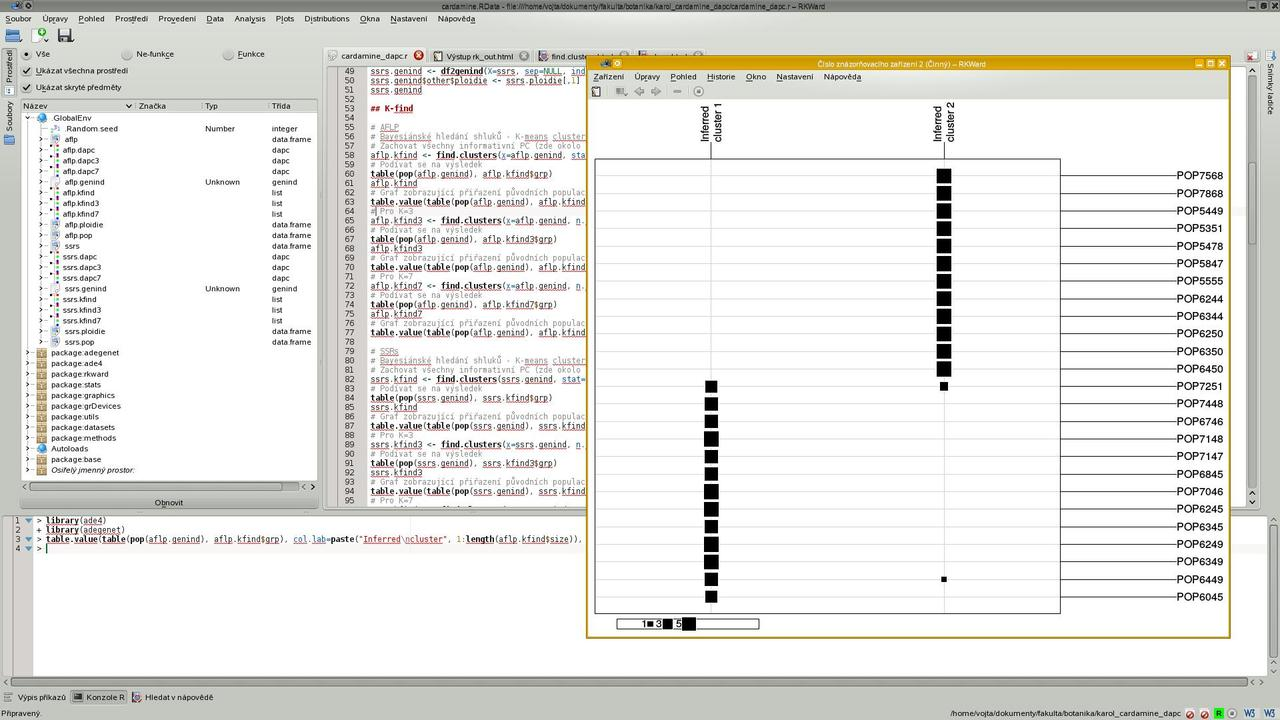
\includegraphics[width=\textwidth]{rkward.jpg}
  \end{center}
\end{frame}

\begin{frame}{RStudio}
  \begin{center}
    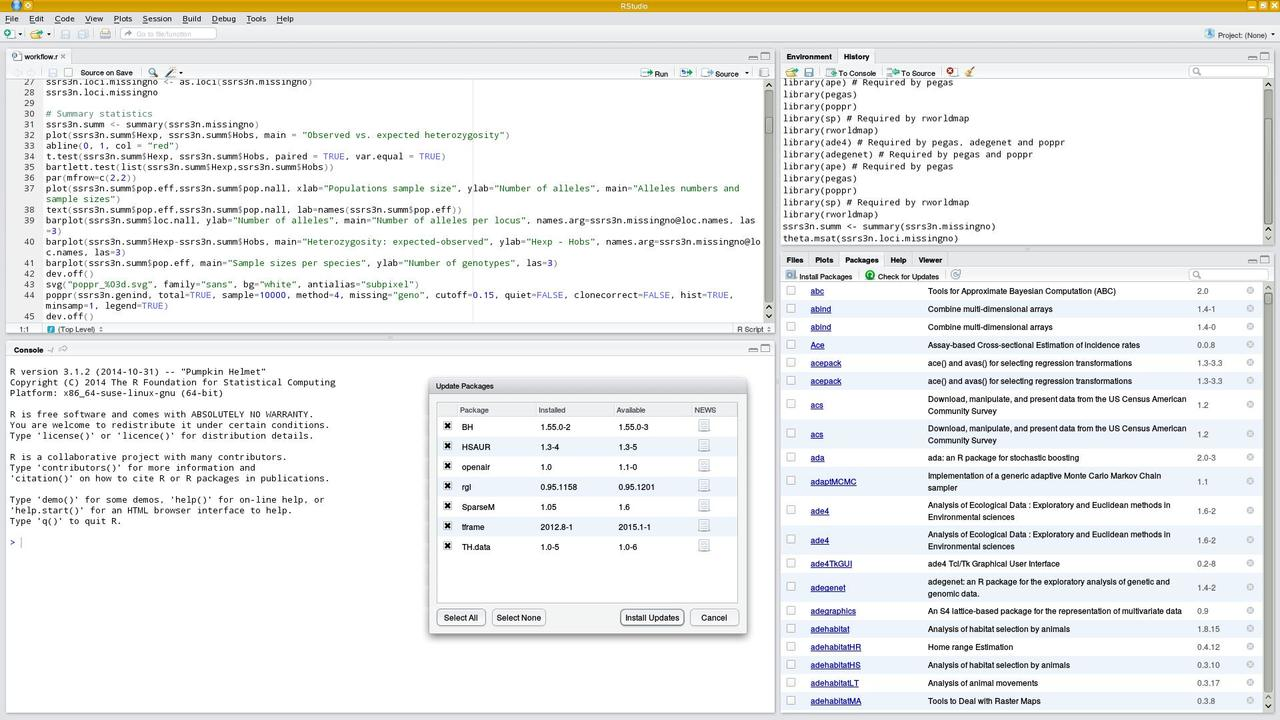
\includegraphics[width=\textwidth]{rstudio.jpg}
  \end{center}
\end{frame}

\subsection{Installation}

\begin{frame}{MS Windows \& Apple Mac OS~X}
  \begin{itemize}
    \item Got to \url{https://cran.r-project.org/}
    \item Download appropriate version and install as usual
    \item Download and install selected GUI (not required, but highly recommended)
    \item Most of packages are available as pre-compiled and can be immediately installed from R -- it is convenient, but usually not tuned for particular computer architecture (type of CPU)
    \item Usually there are some problems every time new version of OS is released -- it takes time to modify and recompile packages for new version of OS
    \item You have to check for new version of R manually
    \item RStudio is available from its \href{https://www.rstudio.com/products/rstudio/download/\#download}{download page}
    \item RKWard is also available for \href{https://rkward.kde.org/RKWard_on_Windows}{Windows} and \href{https://rkward.kde.org/RKWard_on_Mac}{Mac OS~X}, but it requires some work to install it
  \end{itemize}
\end{frame}

\begin{frame}{Linux -- general}
  \begin{itemize}
    \item R, and usually also GUI, is available in repositories -- use standard package management according to distribution
    \item Linux repositories provide automatic updates
    \item Packages are also partially available in repositories and can be installed and updated as usual application or from R
    \item Packages commonly have to be compiled -- R will do it automatically, but install basic Linux packages for building of C, C++, Fortran,~\ldots
    \item Compilation takes longer time and there are sometimes issues with missing dependencies (tools required by particular packages), but it can then provide higher performance\ldots
  \end{itemize}
\end{frame}

\begin{frame}{Linux -- Debian/Ubuntu and derivatives like Linux Mint or Kali Linux}
  \begin{itemize}
    \item Install package \texttt{build-essential} (general tools to compile software, including R packages)
    \item Debian (and derivatives): follow instructions at \url{https://cran.r-project.org/bin/linux/debian/}
    \item Ubuntu (and derivatives): follow instructions at \url{https://cran.r-project.org/bin/linux/ubuntu/}
    \item As \texttt{<my.favorite.cran.mirror>} select \alert{\texttt{https://cran.wu.ac.at/}}, see \alert{CRAN Mirrors} at \url{https://cran.r-project.org/mirrors.html}
    \item Install packages \texttt{R-base} (the R), \texttt{R-base-dev} (required to compile additional R packages -- only some are available in repositories) and optionally \texttt{rkward} and/or \texttt{rstudio}
    \item RStudio is also available from its \href{https://www.rstudio.com/products/rstudio/download/\#download}{download page}
  \end{itemize}
\end{frame}

\begin{frame}{Linux -- openSUSE and SUSE Linux Enterprise}
  \begin{itemize}
    \item See instructions at \url{https://cran.r-project.org/bin/linux/suse/}
    \item Add repository/ies for appropriate version of your distribution
    \begin{itemize}
      \begin{footnotesize}
	\item \url{http://download.opensuse.org/repositories/devel:/languages:/R:/patched/} (daily updated) or/and
	\item \url{http://download.opensuse.org/repositories/devel:/languages:/R:/released/} (updated with new R release)
      \end{footnotesize}
    \end{itemize}
    \item Install packages \texttt{R-base} (the R), \texttt{R-base-devel} (required to compile additional R packages -- only some are available in repositories) and optionally \texttt{rstudio} and/or \texttt{rkward}
    \item Install package \texttt{patterns-openSUSE-devel\_basis} for compilation of R packages when installing them from R (only some R packages are available in repositories)
    \item RStudio is also available from its \href{https://www.rstudio.com/products/rstudio/download/\#download}{download page}
  \end{itemize}
\end{frame}

\begin{frame}{Linux -- RedHat, Fedora and derivatives like CENTOS, Scientific Linux, etc.}
  \begin{itemize}
    \item See instructions at \url{https://cran.r-project.org/bin/linux/redhat/README}
    \item Install packages \texttt{R-core} (the R), \texttt{R-core-devel} (required to compile additional R packages -- only some are available in repositories) and optionally \texttt{rkward}
    \item RStudio is available from its \href{https://www.rstudio.com/products/rstudio/download/\#download}{download page}
  \end{itemize}
\end{frame}

\begin{frame}{Sources of R packages}
  \label{sources}
  \begin{itemize}
    \item R CRAN \url{https://cran.r-project.org/} -- main and largest source of R packages (almost 10,000 packages + many orphaned and archived -- abandoned by developers, might be working)
    \item Bioconductor \url{https://bioconductor.org/} -- mainly bioinformatics packages, genomic data (over 1,400 packages)
    \item R-Forge \url{https://r-forge.r-project.org/} (over 2,000 packages)
    \item RForge \url{https://www.rforge.net/} (much smaller)
    \item And more\ldots
    \item Some packages are available from more resources
    \item Same name for function can be used in different packages (there is no central index) -- to distinguish them call functions like this: \texttt{muscle::read.fasta()} vs. \texttt{seqinr::read.fasta()} -- call function \texttt{read.fasta()} from package \texttt{muscle} \alert{or} \texttt{seqinr} (and their parameters can be different\ldots) -- see further
  \end{itemize}
\end{frame}

\subsection{Let's start with R}

\begin{frame}{First steps in R}{Recommended is usage of GUI (RKWard or RStudio)}
  \begin{multicols}{2}
    \begin{itemize}
      \item Linux (UNIX): open any terminal, type \texttt{R} and hit Enter
      \item Windows and Mac: find it as normal application in menu
      \item Type commands to work\ldots
      \item \alert{Ever wished to be Harry Potter? Secret spells make magic operations~:-)}
      \item Use arrows up and down to navigate in history
      \item \texttt{Ctrl+R} works as reverse search -- searches text in history
    \end{itemize}
    \columnbreak
    \begin{center}
      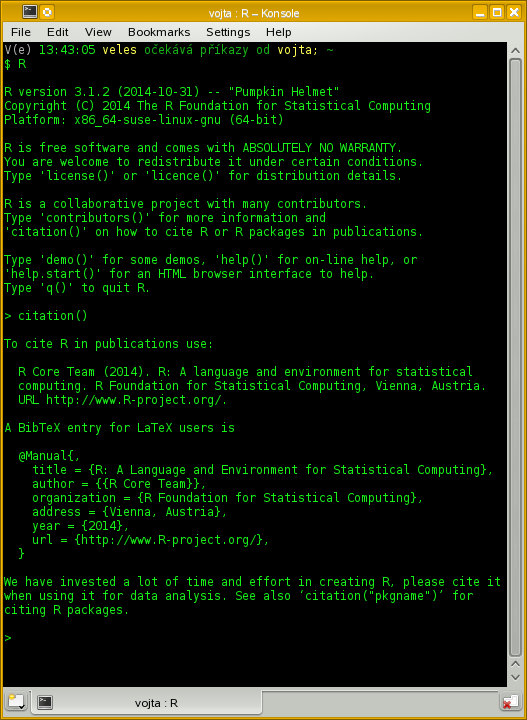
\includegraphics[width=4.5cm]{rkonsole.png}
    \end{center}
  \end{multicols}
\end{frame}

\begin{frame}{How it works}
  \begin{itemize}
    \item General look of R commands:
    \item \splus/function(argument1="SomeName", argument2=SomeVariable, argument3=8)/
    \item \splus/ModifiedObject <- SomeFunction(argument1=MyData, argument2=TRUE)/
    \item New/modified object (with data,~\ldots) is on the left: ``\texttt{<-}'' says to insert result of the function \texttt{SomeFunction} on the right into the object \texttt{ModifiedObject} on the left
    \item Functions have various parameters/arguments (in brackets, separated by comas): \texttt{argument=ItsValue}
    \item Arguments are named -- if you keep order, no need to name them:
    \item \splus/SomeFunction(MyData, TRUE, 123, "SomeName")/
    \item When only some of the arguments are in use, use the names (order doesn't matter any more)
    \item \splus/SomeFunction(argument2=TRUE, argument3=123, argument1=MyData)/
    \item Some arguments are required, some optional
  \end{itemize}
\end{frame}

\begin{frame}[fragile]{Get help in R}
  \begin{spluscode}
    # "#" marks comments - notes within code which are not executed
    help(function) # Help for particular function (package must be loaded)
    ?function # Help for particular function (package must be loaded)
    ??SearchedTerm # Search for the term within all installed packages
    help.search("searched phrase") # Search for the phrase within all
      # installed packages - return list of hits sorted according to
      # type and package (i.e. package::function)
    install.packages("sos") # More comprehensive search from packages
    library(sos)
    findFn("function") # Search for function name
  \end{spluscode}
  \vfil
  \alert{\texttt{?}} shows help for questioned function (in console type \texttt{q} to close it):
  \begin{multicols}{2}
    \begin{itemize}
      \item Name of the package (top left)
      \item Function name (headline)
      \item Description
      \item Usage
      \item Comments on arguments
      \item Details
      \item About author(s)
      \item References to cite
      \item Example code
    \end{itemize}
  \end{multicols}
\end{frame}

\begin{frame}[fragile]{Where we are?}
  \begin{itemize}
    \item In Linux/UNIX, R starts in current directory (use \texttt{cd} to change it before launching R)
    \item \alert{Set and check working directory} in R:
  \end{itemize}
  \begin{spluscode}
    setwd("/some/path/") # Or "~/...". In Windows "C:\..."
    getwd() # Verifies where we are
    dir() # Lists files and folders on the disk
    ls() # Lists currently available R objects
  \end{spluscode}
  \begin{itemize}
    \item In Windows (\textbf{File | working directory}) or in RStudio (\textbf{Session | Set working directory}) set it in menu or by above command
    \item R saves history of commands into file \texttt{.Rhistory} file within working directory (by default hidden in Linux/Mac OS~X)
    \item When closing R by \texttt{q()} you can save all R data in \texttt{.RData} (and command history in \texttt{.Rhistory}) file(s) and it/they can be loaded next time
    \item RStudio and RKWard help with this very much
  \end{itemize}
\end{frame}

\begin{frame}{Importance of working directory}
  \begin{itemize}
    \item Default place to load/save, import/export data/results
    \begin{itemize}
      \item It changes paths -- one of the most common mistakes -- something is not found because of wrong path
      \item Private folder for particular R project (task) prevents unwanted inferences with another tools/projects
    \end{itemize}
    \item Without saving and loading the R data next time, it is not possible to do any longer work or to check the work in the future
    \item \alert{Get used that R \textbf{always} work in some directory and by default saves/loads files there}
    \item RStudio and RKWard also save session information (list of opened files,~\ldots) -- very convenient
    \item Regularly save your work to prevent looses in case of crash or any other accident
  \end{itemize}
\end{frame}

\subsection{Basic operations in R}

\begin{frame}{Types of objects}
  \begin{itemize}
    \item \textbf{Vectors} -- numbers or characters
    \item \textbf{Matrices} -- columns are of same type (numeric, character, etc.) and the same length
    \item \textbf{Arrays} -- like matrices, but with possibly more dimensions
    \item \textbf{Data frames} -- more general -- columns can be of different type
    \item \textbf{Lists} -- ordered collections of objects (vectors, matrices,~\ldots) -- not necessarily of the same type
    \item \textbf{Factors} -- a~vector of levels, e.g. populations, colors, etc.
    \item More ``advanced'' objects to store plots, genetic data,~\ldots
    \begin{itemize}
      \item Commonly called ``\textbf{S3}'' and ``\textbf{S4}'' objects in R terminology
      \item Technically commonly just lists putting together various information
      \item We will meet many of them\ldots
    \end{itemize}
  \item Functions require particular object types -- take care about it
  \end{itemize}
\end{frame}

\begin{frame}{Popular object classes (we are going to use) I}
  \begin{itemize}
    \item \texttt{dist} -- distance matrices
    \item \texttt{genind} -- stores various genetic information for individuals
    \item \texttt{genpop} -- like genind, but on population level
    \item \texttt{genlight} -- variant of genind to store large multiple genomes
    \item \texttt{SNPbin} -- stores large SNP data for single genome
    \item \texttt{DNAbin} -- stores DNA sequences (aligned or not)
    \item \texttt{haplotype} -- unique sequences from DNAbin
    \item \texttt{alignment} -- aligned sequences (seqinr)
    \item \texttt{phyDat} -- ``preparation'' of data for some phylogenetic analysis
    \item \texttt{loci} -- extension of data frame (DF), stores information about loci
    \item \texttt{hclust} -- output of hierarchical clustering, can be converted to phylo
    \item \texttt{treeshape} -- derived from hclust
  \end{itemize}
\end{frame}

\begin{frame}[fragile]{Popular object classes (we are going to use) II}
  \begin{itemize}
    \item \texttt{phylo} -- phylogenetic information, typically trees
    \item \texttt{phylo4} -- derived from phylo (more data), S4 instead of S3
    \item \texttt{matching} -- binary phylogenetic trees
    \item \texttt{haplonet} -- networks without reticulation
    \item \texttt{spca} -- results of sPCA
    \item \texttt{pco}; \texttt{dudi} -- results of PCA, PCoA,~\ldots
    \item \texttt{dapc} -- results of DAPC
    \item and more\ldots~common task is converting among formats\ldots
    \item \ldots not all formats are (easily) convertible among each other\ldots
  \end{itemize}
  To get information about content of each data type see
  \splus/getClassDef("genind") # Or any other class name (of loaded package)/
  There are information about slots within that classes you can access.
\end{frame}

\begin{frame}{Conversions among data types I}
  \begin{tabular}{llll}
    \textbf{From} & \textbf{To} & \textbf{Command} & \textbf{Package}\\
    phylo & phylo4 & \texttt{as(x, "phylo4")} & phylobase\\
    phylo & matching & \texttt{as.matching(x)} & ape\\
    phylo & treeshape & \texttt{as.treeshape(x)} & apTreeshape\\
    phylo & hclust & \texttt{as.hclust(x)} & ape\\
    phylo & prop.part & \texttt{prop.part(x)} & ape\\
    phylo & splits & \texttt{as.splits(x)} & phangorn\\
    phylo & evonet & \texttt{evonet(x, from, to)} & ape\\
    phylo & network & \texttt{as.network(x)} & ape\\
    phylo & igraph & \texttt{as.igraph(x)} & ape\\
    phylo4 & phylo & \texttt{as(x, "phylo")} & phylobase\\
    matching & phylo & \texttt{as.phylo(x)} & ape\\
    treeshape & phylo & \texttt{as.phylo(x)} & apTreeshape\\
    splits & phylo & \texttt{as.phylo(x)} & phangorn
  \end{tabular}
\end{frame}

\begin{frame}{Conversions among data types II}
  \begin{tabular}{llll}
    \textbf{From} & \textbf{To} & \textbf{Command} & \textbf{Package}\\
    splits & networx & \texttt{as.networx(x)} & phangorn\\
    evonet & phylo & \texttt{as.phylo(x)} & ape\\
    evonet & networx & \texttt{as.networx(x)} & ape\\
    evonet & network & \texttt{as.network(x)} & ape\\
    evonet & igraph & \texttt{as.igraph(x)} & ape\\
    haploNet & network & \texttt{as.network(x)} & pegas\\
    haploNet & igraph & \texttt{as.igraph(x)} & pegas\\
    hclust & phylo & \texttt{as.phylo(x)} & ape\\
    hclust & dendrogram & \texttt{as.dendrogram(x)} & stats\\
    DNAbin & character & \texttt{as.character(x)} & ape\\
    DNAbin & alignment & \texttt{as.alignment(x)} & ape\\
    DNAbin & phyDat & \texttt{as.phyDat(x)} & phangorn\\
    DNAbin & genind & \texttt{DNAbin2genind(x)} & adegenet\\
    character & DNAbin & \texttt{as.DNAbin(x)} & ape
  \end{tabular}
\end{frame}

\begin{frame}{Conversions among data types III}
  \begin{tabular}{llll}
    \textbf{From} & \textbf{To} & \textbf{Command} & \textbf{Package}\\
    character & loci & \texttt{as.loci(x)} & pegas\\
    alignment & DNAbin & \texttt{as.DNAbin(x)} & ape\\
    alignment & phyDat & \texttt{as.phyDat(x)} & phangorn\\
    alignment & character & \texttt{as.matrix(x)} & seqinr\\
    alignment & genind & \texttt{alignment2genind(x)} & adegenet\\
    phyDat & DNAbin & \texttt{as.DNAbin(x)} & phangorn\\
    phyDat & character & \texttt{as.character(x)} & phangorn\\
    loci & genind & \texttt{loci2genind(x)} & pegas\\
    loci & data frame & \texttt{class(x) <- "data.frame"} & --- \\
    genind & loci & \texttt{genind2loci(x)} & pegas\\
    data frame & phyDat & \texttt{as.phyDat(x)} & phangorn\\
    data frame & loci & \texttt{as.loci(x)} & pegas\\
    data frame & genind & \texttt{df2genind(x)} & adegenet\\
    matrix & phyDat & \texttt{as.phyDat(x)} & phangorn
  \end{tabular}
\end{frame}

\begin{frame}[fragile]{Basic operations with data I}
  \begin{spluscode}
    x <- c(5, 6, 7, 8, 9) # Creates vector (see also ?rep)
    x # Print "x" content
    c() # Is generic function to concatenate objects into new one
    length(x) # Length of the object - for matrices and DF use dim()
    str(x) # Information about structure of the object
    mode(x) # Gets type of storage mode of the object
    class(x) # Shows class of the object
    x[2] # Shows second element of the object
    x <- x[-5] # Removes fifth element
    y <- matrix(data=5:20, nrow=4, ncol=4) # Creates a matrix
    is.matrix(y) # Is it matrix? Try is.<TAB><TAB>
    # TAB key shows available functions and objects starting by typed text
    y # Prints the matrix
    y[,2] # Prints second column
    y[3,] # Prints third row
    y[4,3] # Prints element from fourth row and third column
    x <- y[2,] # Replaces "x" by second row of "y" (no warning)
    # R doesn't ask neither notifies when overwriting objects! Be careful!
  \end{spluscode}
\end{frame}

\begin{frame}[fragile]{Basic operations with data II}
  \begin{spluscode}
    rm(x) # Deletes x
    y[,1:3] # Prints first through third column of the matrix
    y[3,] <- rep(x=20, each=4) # Replaces third line by value of 20
    y[y==20] <- 10 # If value of y's element is 20, replace it by 10
    summary(y) # Basic statistics - according to columns
    colnames(y) <- c("A", "B", "C", "D") # Set column names
    # Objects and functions are without quotation marks; files and text with
    colnames(y) # Prints column names, use rownames() in very same way
    y[,"C"] # Prints column C (R is case sensitive!)
    t(y) # Transposes the matrix
    y <- as.data.frame(y) # Turns into DF (see other functions as.*)
    y[y==17] <- "NA" # Removes values of 17 (NA = not available = missing)
    y$B # Gets variable B of data frame y ($ works similarly in S3 objects)
    save(list=ls(), file="test.RData") # Saves all objects during the work
    load("test.RData") # Loads saved R environment with all objects
    # When loading saved project, you have to load again libraries and
    # scripts (see further), data objects are restored
  \end{spluscode}
\end{frame}

\subsection{Packages for our work}

\begin{frame}{Repositories}
  \begin{itemize}
    \item Repositories (internet directories full of R packages -- slide~\ref{sources}) can be set via \texttt{options(repos=c())} or as \texttt{repos} parameter for each \texttt{install.packages()} command (slide~\ref{repos} and onward)
    \item Repositories doesn't have to be set as global options, e.g. Bioconductor has its own way to manage packages
  \end{itemize}
  \begin{block}{Installation of packages in GUI}
    \begin{itemize}
      \item \textbf{RStudio:} set repositories by command from slide~\ref{repos} and in bottom right pane select \textbf{Packages} and click on \textbf{Install Packages\ldots}
      \item \textbf{RKWard:} go to menu \textbf{Settings | Configure 'RKWard'} and select \textbf{R-Packages}. Add URLs of repositories from slide~\ref{repos}. \textbf{OK}. Go to menu \textbf{Settings | Manage R packages and plugins\ldots}, click to \textbf{Install\ldots}, select and install desired packages\ldots
    \end{itemize}
  \end{block}
\end{frame}

\begin{frame}{Theory for packages and their management}
  \begin{itemize}
    \item Standalone plain R doesn't have enough tools for most of scientific disciplines -- only basic methods and tools for programmers, including for package management
    \item Users/developers contribute by making extra packages extending computational possibilities -- one of biggest R advantages -- it then has unlimited possibilities
    \item R has infrastructure for maintaining (for developers) and installing (for users) packages -- the \href{https://cran.r-project.org/}{CRAN} repository
    \item For various reasons, some people build their own infrastructures to maintain and install R packages -- compatible with R, bud separated
    \item User has basically two options
    \begin{enumerate}
      \item Set all repositories in R and use basic commands to install packages (slide~\ref{repos})
      \item Specify non-CRAN repository every time installing from it (e.g. slide~\ref{sources-diff}) or use special tools (e.g. for \href{http://bioconductor.org/install/}{Bioconductor} -- slide~\ref{bioc})
    \end{enumerate}
  \end{itemize}
\end{frame}

\begin{frame}[fragile]{Set repositories}
  \label{repos}
  \begin{spluscode}
    # Basic package installation
    install.packages("PackageName") # Case sensitive!
    ?install.packages # Shows all available parameters (options)
    # We will need extra repositories. For Bioconductor keep version for
    # your R version (BioC 3.4 for R 3.4, see https://bioconductor.org/).
    options(repos=c("https://cran.wu.ac.at/", "https:/rforge.net/",
      "https://r-forge.r-project.org/", "https://bioconductor.
      statistik.tu-dortmund.de/packages/3.4/bioc", "https://bioconductor.
      statistik.tu-dortmund.de/packages/3.4/data/annotation", 
      "https://bioconductor.statistik.tu-dortmund.de/packages/3.4/data/
      experiment", "https://bioconductor.statistik.tu-dortmund.de/
      packages/3.4/extra"))
    getOption("repos") # Shows actual repositories
    options() # Generic function to modify various settings
    ?options # Gives details
  \end{spluscode}
  \begin{itemize}
    \item \alert{Keep newest version of R and and newest versions of packages!}
    \item Installation of multiple packages may sometimes fail -- install then packages in smaller groups or one by one
  \end{itemize}
\end{frame}

\begin{frame}[fragile]{Install needed packages}
  \begin{spluscode}
    # Simplest usage
    install.packages("PackageName") # Case sensitive!
    # Install packages needed for the course
    install.packages(pkgs=c("BiocGenerics", "Biostrings", "Geneland",
      "IRanges", "MASS", "PBSmapping", "ParallelStructure", "RandomFields",
      "RandomFieldsUtils", "RgoogleMaps", "Rmpi", "S4Vectors",
      "TeachingDemos", "XML", "XVector", "ade4", "adegenet", "adephylo",
      "akima", "ape", "brew", "caper", "colorspace", "combinat", "corrplot",
      "diveRsity", "fields", "geiger", "ggplot2", "gplots", "hierfstat",
      "lattice", "mapdata", "mapproj", "maps", "maptools", "muscle",
      "mvtnorm", "nlme", "pegas", "permute", "phangorn", "phylobase",
      "phytools", "picante", "plotrix", "polysat", "poppr", "rworldmap",
      "seqinr", "shiny", "sos", "sp", "spdep", "spam", "vegan"),
      repos=getOption("repos"), dependencies=TRUE)
    ?install.packages # See for more options
    # Installed packages are "inactive" - the mus by loaded to use them:
    library(package) # Loads installed package (we will do it on the fly)
    update.packages(repos=getOption("repos")) # Updates installed packages
  \end{spluscode}
\end{frame}

\begin{frame}[fragile]{Install packages without setting the repositories}
  \begin{itemize}
   \item If repositories from slide~\ref{repos} are not set (for any reason), it is possible to install in several steps packages from main repository (CRAN) and from another sources (following slides)
   \item This is the basic and default the most common usage
  \end{itemize}
  \begin{spluscode}
    install.packages(pkgs=c("Geneland", "MASS", "PBSmapping",
      "RandomFields", "RandomFieldsUtils", "RgoogleMaps", "Rmpi",
      "TeachingDemos", "XML", "ade4", "adegenet", "adephylo", "akima",
      "ape", "brew", "caper", "colorspace", "combinat", "corrplot",
      "diveRsity", "fields", "geiger", "ggplot2", "gplots", "hierfstat",
      "lattice", "mapdata", "mapproj", "maps", "maptools", "mvtnorm",
      "nlme", "pegas", "permute", "phangorn", "phylobase", "phytools",
      "picante", "plotrix", "polysat", "poppr", "rworldmap", "seqinr",
      "shiny", "sos", "sp", "spdep", "spam", "vegan"), dependencies=TRUE)
    update.packages(ask=FALSE) # Update installed (CRAN by default) packages
  \end{spluscode}
\end{frame}

\begin{frame}[fragile]{Install phyloch package}{Example of installation of package not available in any repository}
  \label{phyloch}
  \begin{itemize}
    \item Check \url{http://www.christophheibl.de/Rpackages.html} 
    \item Package phyloch is similar to \href{https://cran.r-project.org/web/packages/ips/}{ips} from same author (but some functions behave differently) -- both are great for usage of external applications within R
  \end{itemize}
  \begin{spluscode}
    # If not done already, install required packages first
    install.packages(pkgs=c("ape", "colorspace", "XML"),
      dependencies=TRUE)
    # It is possible to specify direct path
    # Local or web URL - be careful about correct path) to package source
    install.packages(pkgs="http://www.christophheibl.de/
      phyloch_1.5-3.tar.gz", repos=NULL, type="source")
  \end{spluscode}
\end{frame}

\begin{frame}[fragile]{Bioconductor}
  \label{bioc}
  \begin{itemize}
    \item Tools for analysis of genomic data, see \url{https://bioconductor.org/}
    \item To install it, add appropriate repositories (repository use to have same version number as R -- change them accordingly when upgrading R) or \textbf{use Bioconductor's special function} (recommended by Bioconductor):
  \end{itemize}
  \begin{spluscode}
    # Load basic Bioconductor function
    source("https://bioconductor.org/biocLite.R")
    ?biocLite # Get help how to use it
    # Install packages
    biocLite(c("package1", "package2", "..."))
    biocLite() # Update Bioconductor packages (within same R version)
    # Upgrades installed Bioconductor packages to new R release
    biocLite("BiocUpgrade") # E.g. from R 3.2 to 3.3
  \end{spluscode}
  \begin{itemize}
    \item Explore available packages: \url{https://bioconductor.org/packages/release/BiocViews.html}
  \end{itemize}
\end{frame}

\begin{frame}[fragile]{Bioconductor packages for the course}
  \begin{itemize}
    \item If repositories are not set via command on slide~\ref{repos}, it is possible to use Bioconductor's own installation method using function \texttt{biocLite}
    \item If Bioconductor repositories are set manually, user must select correct version number
    \item List of available Bioconductor mirrors is at \url{https://bioconductor.org/about/mirrors/}% -- for us, \href{https://bioconductor.statistik.tu-dortmund.de/}{Technische Universität Dortmund} is the closest
  \end{itemize}
  \begin{spluscode}
    # Install needed Bioconductor packages
    biocLite(pkgs=c("BiocGenerics", "Biostrings", "IRanges", "S4Vectors",
      "XVector", "muscle"))
    # From time to time update Bioconductor packages
    biocLite()
    # When upgrading to new version of R (e.g. from 3.2 to 3.3) upgrade by
    biocLite("BiocUpgrade")
  \end{spluscode}
\end{frame}

\begin{frame}[fragile]{Bioconductor and others -- differences from another repositories}
  \label{sources-diff}
  \begin{spluscode}
    # Standard installation
    install.packages(pkgs=c("adegenet", "poppr", "phytools"))
    update.packages(ask=FALSE) # Update packages
    # Installation from custom repository (example for our course)
    install.packages(pkgs="ParallelStructure",
      repos="https://r-forge.r-project.org")
    ?install.packages # See help for details
    # Bioconductor - if https fails, use http
    source("https://bioconductor.org/biocLite.R")
    ?biocLite
    biocLite(pkgs=c("Biostrings", "seqinr")) # Install package(s)
    biocLite() # Update Bioconductor packages
  \end{spluscode}
  \begin{itemize}
    \item Bioconductor has it own installation method
    \item Its repositories can be set in R and its packages can then be installed as usually with \texttt{install.paskages()} --- Although Bioconductor developers recommend usage of \texttt{biocLite} function\ldots
  \end{itemize}
\end{frame}

\begin{frame}{Non-R software}
  \begin{itemize}
    \item We use several software packages outside R
    \begin{itemize}
      \item R functions can use this software
      \item External software can be used (depending on R package) to create/modify R object, or just as different method for (batch) usage of the software
      \item User must install this software manually
    \end{itemize}
    \item Structure \url{http://pritchardlab.stanford.edu/structure.html} (optionally also \href{https://web.stanford.edu/group/rosenberglab/clumpp.html}{CLUMPP} and \href{https://web.stanford.edu/group/rosenberglab/distruct.html}{distruct} -- not part of the course)
%     \item PHYLIP \url{http://evolution.genetics.washington.edu/phylip/} % TODO Rphylip
    \item MAFFT \url{http://mafft.cbrc.jp/alignment/software/}
    \item MUSCLE \url{http://www.drive5.com/muscle/}
    \item Clustal (W/X; Omega is not used in the course) \url{http://clustal.org/}
  \end{itemize}
\end{frame}

\section{Data}

\begin{frame}[allowframebreaks]{Our data\ldots}
  \begin{itemize}
    \item Work with microsatellites is in most cases (except some methods taking advance from microsatellite mutational nature) same as with presence-absence data and methods can handle both data types in nearly same fashion
    \begin{itemize}
      \item Examples are shown mainly with microsatellites, but AFLP and another presence-absence (1/0) data are used in same way -- try it
    \end{itemize}
    \item Distance-based methods are same regardless input data on the beginning (microsatellites, AFLP, DNA sequences,~\ldots)
    \item Extraction of SNP from DNA is useful in case of huge datasets -- for smaller datasets it is not necessary
  \end{itemize}
  \begin{block}{Always save your work!}
    \alert{We will use data objects during whole course -- all the time save your workspace!} Use possibilities of your GUI or \texttt{save}/\texttt{load} functions.
  \end{block}
\end{frame}

\begin{frame}[allowframebreaks]{Brief overview of molecular data types}{Sorted with respect to usage in R}
  \begin{itemize}
    \item Isozymes -- forms of proteins differing in electrophoresis by their weight and/or charge
    \begin{itemize}
      \item Typically coded as presence/absence (1/0) data
    \end{itemize}
    \item Fragmentation data -- length polymorphism
    \begin{itemize}
      \item Codominant data -- e.g. microsatellites (SSRs -- Simple Sequence Repeats)
      \begin{itemize}
	\item Variability in number of short (usually 1-3~bp) oligonucleotide repeats (ATAT vs. ATATAT, typically ca. 25-250 repeats) bordered by unique primer sequences
	\item Very variable, fast evolving, species-specific primers needed
	\item Mainly for population genetics, relationships among closely related species
	\item Similarly ISSRs (Inter Simple Sequence Repeats)
      \end{itemize}
      \item Presence/absence (1/0) dominant data
      \begin{itemize}
	\item The allele \textbf{is} or \textbf{is not} present  -- it is impossible to distinguish heterozygots from dominant homozygots
	\item AFLP (Amplified Fragment Length Polymorphism) -- very variable, technically complicated, nowadays bit expensive and outdated
	\item Simpler methods RAPD (Random Amplified Polymorphic DNA) and PCR-RFLP (Polymerase Chain Reaction-Restriction Fragment Length Polymorphism) are not used anymore at all
      \end{itemize}
    \end{itemize}
    \item Protein sequences -- not used in the course
    \begin{itemize}
      \item Apart similar usage as with DNA/RNA (sequence analysis) it is possible to work with the structure and conformation of the proteins
      \item R has plenty of packages for specialized protein analyses
    \end{itemize}
    \item Nucleic acid sequences (in nearly any form) -- DNA or RNA
    \begin{itemize}
      \item From ``classical'' Sanger sequencing -- long individual reads
      \item From modern HTS (NGS) -- 454 pyrosequencing, Illumina,~\ldots
	\begin{itemize}
	  \item Probably most used are RADseq scanning whole genome, HybSeq using specific probes to sequence only single/low-copy nuclear markers, Genome Skimming getting the most abundant part of the genome (plastid and mitchodrial sequences and ITS1-5.8S rRNA-ITS2 region); and their variants
	  \item There are special tools to process raw data from the machines -- not part of the course
	\end{itemize}
      \item Whole sequences (probes/loci or longer assembled regions) or SNPs (Single Nucleotide Polymorphism -- only polymorphic sites are retained)
    \end{itemize}
    \item Most of methods are mathematically well defined for haploids and/or diploids, higher ploidies or mixing of ploidies is not always possible
    \item Most of methods shown in the course work with more data types -- not everything is shown
    \item For details about the molecular markers check specialized course like \href{https://is.cuni.cz/studium/predmety/index.php?do=predmet&kod=MB120P44}{Use of molecular markers in plant systematics and population biology}
  \end{itemize}
\end{frame}

\begin{frame}[allowframebreaks]{Notes about paths to import the data}
  \label{path}
  \begin{itemize}
    \item Generally, R can accept nearly any local or web location
    \item If unsure where you are, open any file manager, go to the R working directory (verify with \texttt{getwd()} and \texttt{dir()}) and verify where everything is
    \item Web locations start with \texttt{https://}, \texttt{http://} or \texttt{ftp://}, e.g. \texttt{FileParameter="https://server.cz/directory/file.txt"}
    \item Local paths (within one computer) can be absolute or relative
    \begin{itemize}
      \item Absolute paths start from the top of files hierarchy: on UNIX (Linux, Mac OS~X,~\ldots) it use to look like \texttt{/home/USER/}, on Windows like \texttt{C:\textbackslash} (e.g. \texttt{FileParameter="/path/to/some/file.txt"})
      \item Relative paths start in current directory (so \textbf{no} with \texttt{/} or \texttt{C:})
      \begin{itemize}
	\item In the easiest case the input file is in same directory as is R's working directory -- verify by \texttt{getwd()} and \texttt{dir()} -- you then need to specify only the filename (e.g. \texttt{FileParameter="SomeFile.txt"})
	\item For subdirectory start with its name (\textbf{no} with \texttt{/} or \texttt{C:}), e.g. \texttt{FileParameter="subdirectory/another/directory/file.txt"}
	\item When going directory up, use one \texttt{..} for each level, e.g. \texttt{FileParameter="../upper/directory/file.txt"}
	\item On UNIX (Mac OS~X, Linux,~\ldots) tilde \texttt{\textasciitilde} means user's home directory (e.g. \texttt{/home/USER/}), so \texttt{FileParameter="\textasciitilde/some/file.txt"} is same as \texttt{FileParameter="/home/USER/some/file.txt"}
      \end{itemize}
      \item If loading data from computer, carefully check the paths or use function \texttt{file.choose()} to interactively pick up the file anywhere in the computer -- it can replace nearly any filename parameter (e.g. \texttt{FileParameter="file.choose()"}
    \end{itemize}
    \item Some R functions have problems with spaces and special (non-alphanumeric and accented) characters -- try to avoid them
    \item One of the most common source of errors -- \textbf{when the command fails, double check paths} (and Internet connection, if applicable) -- for another common problems see slide~\ref{problems}
  \end{itemize}
\end{frame}

\begin{frame}[fragile]{Population genetics and phylogenetics in R}{Microsatellites, AFLP, SNP \& sequences}
  \begin{multicols}{2}
    \begin{itemize}
      \item Now we will use mainly packages \href{http://adegenet.r-forge.r-project.org/}{adegenet} and \href{http://grunwaldlab.cgrb.oregonstate.edu/poppr-r-package-population-genetics}{poppr}
      \item Other important genetic packages: \href{http://ape-package.ird.fr/}{ape}, \href{http://pbil.univ-lyon1.fr/ADE-4/}{ade4} and \href{http://ape-package.ird.fr/pegas.html}{pegas}
      \item Dominant/co-dominant marker data of any ploidy level including SSRs, SNP, and AFLP are analyzed in same way
      \item Most of methods are available for polyploids (although not all)
      \item Some methods are unavailable for dominant (presence/absence) data
      \item Mixing of ploidy levels is tricky (but possible) -- it doesn't matter when data are encoded as PA, otherwise it is mathematically problematic
    \end{itemize}
    \begin{spluscode}
      library(ape)
      library(ade4)
      library(adegenet)
      library(pegas)
      library(poppr)
    \end{spluscode}
  \end{multicols}
\end{frame}

\subsection{Microsatellites}

\begin{frame}[fragile]{Load data}
  \vfill
  \textbf{Source data:}
  \vfill
  \begin{spluscode}
        pop  msta93 msta101 msta102 msta103 msta105 msta131 ...
    H01 He  269/269 198/198 221/223 419/419 197/197 196/196 ...
    H02 He  275/283 198/198 221/223 419/419 193/193 168/190 ...
    ... ... ...     ...     ...     ...     ...     ...     ...
  \end{spluscode}
  \vfill
  \textbf{Loading the data:}
  \vfill
  \begin{spluscode}
    # Load training data (Taraxacum haussknechtii from Macedonia)
    hauss.loci <- read.loci(file="https://soubory.trapa.cz/rcourse/
      haussknechtii_ssrs.txt", header=TRUE, loci.sep="\t", allele.sep="/",
      col.pop=2, col.loci=3:14, row.names=1) # \t means TAB key
    # Data control
    hauss.loci
    print(hauss.loci, details=TRUE)
  \end{spluscode}
  \vfill
  \begin{footnotesize}
    First line starts with empty cell (if \textbf{header} is presented), there can be any extra column, take care about \texttt{col.loci}. \texttt{row.names} are individual names (first column). Take care about \texttt{loci.sep} (here TAB -- \texttt{\textbackslash t}) and \texttt{allele.sep} (here \texttt{/}) according to data formatting.
  \end{footnotesize}
  \vfill
\end{frame}

\begin{frame}[fragile]{Prepare genind object for analysis and load coordinates}
  \vfill
  \begin{spluscode}
    # Conversion of loci to genind - used for many analysis
    hauss.genind <- loci2genind(hauss.loci)
    # See population names
    pop(hauss.genind)
    hauss.genind$pop # "$" separates extra slots within object
  \end{spluscode}
  \vfill
  \textbf{Source data:}
  \vfil
  \begin{spluscode}
    Ind  lon      lat
    H01  21.3333  41.1
    ...  ...      ...
  \end{spluscode}
  \vfill
  \hrule
  \vfill
  \begin{spluscode}
    # Read coordinates
    hauss.coord <- read.csv("https://soubory.trapa.cz/rcourse/
      haussknechtii_coordinates.csv", header=TRUE, sep="\t",
      quote="", dec=".", row.names=1)
    hauss.coord
  \end{spluscode}
  \vfil
  \begin{itemize}
    \item Coordinates can be in any projection or scale -- according to aim
    \item Take care about parameters of \texttt{read.csv()}! See \texttt{?read.csv} for details
  \end{itemize}
  \vfill
\end{frame}

\begin{frame}[fragile]{Add coordinates to genind and create genpop object}
  \begin{spluscode}
    # Add coordinates - note identification of slots within object
    hauss.genind$other$xy <- hauss.coord
    # See result
    hauss.genind$other$xy
    hauss.genind
    # Conversion to genpop - for population-level analysis
    hauss.genpop <- genind2genpop(hauss.genind, process.other=TRUE)
    # See result
    hauss.genpop
    # Removes missing data - see ?missingno for types of dealing them
    # Use with caution! It modifies original data!
    hauss.genind.cor <- missingno(pop=hauss.genind, type="mean", cutoff=0.1,
      quiet=FALSE)
    # Convert corrected genind to loci
    hauss.loci.cor <- genind2loci(hauss.genind.cor)
    # Writes loci file to the disk
    write.loci(hauss.loci.cor, file="hauss.loci.cor.txt",
      loci.sep="\t", allele.sep="/")
  \end{spluscode}
\end{frame}

\begin{frame}[fragile]{Import existing data set from popular software}
  \begin{spluscode}
    read.genalex() # poppr - reads *.csv file
    read.fstat() # adegenet - reads *.dat files, only haploid/diploid data
    read.genetix() # adegenet - reads *.gtx files, only ha/diploid data
    read.genepop() # adegenet - reads *.gen files, only ha/diploid data
    read.structure() # adegenet - reads *.str files, only ha/diploids
    import2genind() # adegenet - more automated version of above functions
  \end{spluscode}
  \begin{block}{One function rules them all\ldots}
    All those functions (including \texttt{read.loci()} and \texttt{read.csv()}) are only modifications of \textbf{\texttt{read.table()}}. You can use it directly to import any data. Look at \texttt{?read.table} and play with it. Take care about parameters. Does the table use quotes to mark cell (e.g. \texttt{quote="\textbackslash ""})? How are columns separated (e.g. \texttt{sep="\textbackslash t"})? Is there a~header with names of populations/loci/whatever (\texttt{header=T/F})? What is decimal separator (e.g. \texttt{dec="."})? Are there row names (used typically as names of individuals; e.g. \texttt{row.names=1})? \alert{Check data after import!}
  \end{block}
\end{frame}

\begin{frame}[fragile]{Import of polyploid microsatellites}
  \vfill
  \begin{itemize}
    \item \texttt{adegent}, \texttt{poppr} and related packages can for most of functions handle any ploidy level (including mixing of ploidy levels, but not for all analysis)
    \item \texttt{polysat} package can handle mixed ploidy levels for microsatellites, but range of methods is limited
    \item As for AFLP, we need two files: the data matrix and individual's populations (it can be combined in one file -- next slide)
  \end{itemize}
  \vfill
  \textbf{Triploid microsatellite data:}
  \vfil
  \begin{spluscode}
           msat58      msat31      msat78      msat61      ...
    ala1   124/124/124 237/237/237 164/164/172 136/136/138 ...
    ala2   124/124/124 237/237/237 164/164/172 136/136/138 ...
    ala4-1 124/124/124 237/237/237 164/164/172 136/136/138 ...
    ...    ...         ...         ...         ...         ...
  \end{spluscode}
  \vfil
  \begin{footnotesize}
    Triploid species of \textit{Taraxacum} sect. \textit{Taraxacum}
  \end{footnotesize}
  \vfill
\end{frame}

\begin{frame}[fragile]{How to import polyploid microsatellites}
  \begin{spluscode}
    # Import of table is as usual. Last column contains populations
    tarax3n.table <- read.table("http://soubory.trapa.cz/rcourse/
      tarax3n.txt", header=TRUE, sep="\t", quote="", row.names=1)
    # Check the data
    tarax3n.table
    class(tarax3n.table)
    dim(tarax3n.table)
    # See parameter "X" - we don't import whole tarax3n.table as last column
    # contains populations - this column we use for "pop" parameter (note
    # different style of calling the column - just to show the possibility).
    # Check "ploidy" and "ncode" (how many digits code one allele - must be
    # same everywhere). See ?df2genind for more details.
    tarax3n.genind <- df2genind(X=tarax3n.table[,1:6], sep="/", ncode=3,
      pop=tarax3n.table[["pop"]], ploidy=3, type="codom")
    # See resulting genind object
    tarax3n.genind
    summary(tarax3n.genind)
  \end{spluscode}
\end{frame}

\subsection{AFLP}

\begin{frame}[fragile]{Import of AFLP data -- background}
Source data (two files -- AFLP data with individual names and populations)
\begin{multicols}{2}
  \textbf{AFLP or any other presence/absence data:}
  \begin{spluscode}
        L1 L2 L3 L4 L5 L6 L7 L8 L9 ...
    Ind1 0 0 1 1 1 0 0 0 1 ...
    IndG 0 0 1 1 0 0 0 0 0 ...
    ...  ...  ...
  \end{spluscode}
  \begin{footnotesize}
    AFLP data of \textit{Cardamine amara} group
  \end{footnotesize}
\textbf{Individual's populations:}
  \begin{spluscode}
    POP
    pop1
    popZ
    ...
  \end{spluscode}
  \begin{footnotesize}
    Just list of populations for respective individuals\ldots
  \end{footnotesize}
  \columnbreak
  \begin{itemize}
    \item Use any names, just keep one word (no spaces) and don't use special characters
    \item Keep names of loci as simple as possible, there are some issues when they contain dots
    \item As soon as one line of data = one individual, ploidies and their mixing doesn't matter
    \item Not all methods are available/meaningful for PA
  \end{itemize}
\end{multicols}
\end{frame}

\begin{frame}[fragile]{Import of AFLP data -- the code}
  \begin{spluscode}
    amara.aflp <- read.table(file="https://soubory.trapa.cz/rcourse/
      amara_aflp.txt", header=TRUE, sep="\t", quote="")
    amara.aflp
    dim(amara.aflp)
    class(amara.aflp) # Must be matrix or data frame
    # Populations - just one column with population names for all inds
    amara.pop <- read.table(file="https://soubory.trapa.cz/rcourse/
      amara_pop.txt", header=TRUE, sep="\t", quote="")
    amara.pop
    # You can use just one file, where populations are in last column and
    # in df2genind() use for example X=aflp[,1:XXX] and pop=aflp[,YYY]
    # Create genind object - ind.names and loc.names are taken from X
    aflp.genind <- df2genind(X=amara.aflp, sep="", ind.names=NULL,
      loc.names=NULL, pop=amara.pop[,1], missing=NA, type="PA")
    indNames(aflp.genind) <- amara.aflp[,1] # Add individual names
    aflp.genind
    summary(amara.aflp)
    # You can add any other variables into genind$other$XXX
  \end{spluscode}
\end{frame}

\subsection{Notes about data}

\begin{frame}[fragile]{Another data manipulation}
  \begin{itemize}
    \item SNPs can be into genind imported in same way as AFLP (PA)
  \end{itemize}
  \begin{spluscode}
    genind2df() # adegenet - export into data frame
    genind2genalex() # poppr - export for genalex
    splitcombine() # poppr - edits population hierarchy
    popsub() # poppr - extracts only selected population(s)
    clonecorrect() # poppr - corrects for clones
    informloci() # poppr - removes uninformative loci
    seppop() # adegenet - separates populations from genind or genlight
    seploc() # adegenet - splits genind, genpop or genlight by markers
    alleles2loci() # pegas - transforms a matrix of alleles into "loci"
    # seppop and seploc return lists of genind objects - for further
    # analysis using special functions to work on lists (see further)
    # read manual pages (?...) of the functions before usage
  \end{spluscode}
  \begin{itemize}
    \item \texttt{alleles2loci()} is very useful when each allele is in separated columns (not like in our case where one column contains one loci with all alleles) -- saves time needed to change input file formatting
  \end{itemize}
\end{frame}

\begin{frame}{Notes about getting data into R}
  \begin{itemize}
    \item When importing fragmentation data, we somehow use function \texttt{read.table()} -- it is important to understand it
    \item I~recommend to use TAB (TSV -- tab separated values; encoded as \texttt{\textbackslash t} in R) to separate columns (no quotation marks, no commas)
    \item When importing microsatellites, all alleles \textbf{must} have same number of digits. Separate alleles by ``\texttt{/}'', ``\texttt{|}'' or something similar and correctly specify it in \texttt{read.loci()} or \texttt{df2genind()} (or read the data with \texttt{read.table()}, convert into matrix and use \texttt{alleles2loci()})
    \item \textbf{Do not use} underscores (``\texttt{\_}'') or minuses to name objects in R -- only numbers, Latin letters or dots
    \item \texttt{read.loci()} sometimes doesn't work correctly on AFLP or polyploid microsatellites -- try \texttt{read.table()} instead\ldots
    \item Genind object (since Adegenet version 2) is able to store mixed ploidy data, but not all analysis are able to handle that\ldots
  \end{itemize}
\end{frame}

\subsection{DNA sequences, SNP}

\begin{frame}[fragile]{Import of DNA sequence data I}
  \begin{spluscode}
    # Reading FASTA (read.dna() reads also another formats, see ?read.dna)
    # Sequences of flu viruses from various years from USA
    # (Adegenet toy data)
    usflu.dna <- read.dna(file="http://adegenet.r-forge.r-project.org/
      files/usflu.fasta", format="fasta")
    class(usflu.dna) # Check the object
    usflu.dna # Check the object
    # Another possibility (only for FASTA alignments, same result):
    usflu.dna2 <- fasta2DNAbin(file="http://adegenet.r-forge.r-project.org
      /files/usflu.fasta") # Normally keeps only SNP - see ?fasta2DNAbin
    class(usflu.dna2) # Check the object
    usflu.dna2 # Check the object
    as.character(usflu.dna2)[1:5,1:10] # Check the object
    dim(usflu.dna2) # Does it have correct size?
    # Read annotations
    usflu.annot <- read.csv("http://adegenet.r-forge.r-project.org/files/
      usflu.annot.csv", header=TRUE, row.names=1)
    head(usflu.annot) # See result
  \end{spluscode}
\end{frame}

\begin{frame}[fragile]{Import of DNA sequence data II}
  \begin{spluscode}
    # Convert DNAbin to genind - only polymorphic loci (SNPs) are retained
    # When converting DNAbin to genind, the sequences must be aligned!
    usflu.genind <- DNAbin2genind(x=usflu.dna, pop=usflu.annot[["year"]])
    # read.fasta() from seqinr package reads DNA or AA in FASTA format and
    # returns a list (DNAbin is for us now better choice)
    usflu.dna3 <- seqinr::read.fasta(file="http://adegenet.r-forge.
      r-project.org/files/usflu.fasta", seqtype="DNA")
    class(usflu.dna3)
    length(usflu.dna3) # How many sequences we have in the list
    usflu.dna3
    # Convert into DNAbin class (technically, DNAbin is a list)
    class(usflu.dna3) <- "DNAbin"
    # Read sequence data in NEXUS
    read.nexus.data(file="sequences.nex")
  \end{spluscode}
  \begin{itemize}
    \item RNA or protein sequences can be handed in same way
  \end{itemize}
\end{frame}

\begin{frame}[fragile]{Import sequences from GenBank}
  \begin{itemize}
    \item Data from \url{https://www.ncbi.nlm.nih.gov/popset/608602125} (\textit{Meles meles})
  \end{itemize}
  \begin{spluscode}
    # Importing sequences according to sequence ID
    meles.dna <- read.GenBank(c("KJ161355.1", "KJ161354.1", "KJ161353.1",
      "KJ161352.1", "KJ161351.1", "KJ161350.1", "KJ161349.1", "KJ161348.1",
      "KJ161347.1", "KJ161346.1", "KJ161345.1", "KJ161344.1", "KJ161343.1",
      "KJ161342.1", "KJ161341.1", "KJ161340.1", "KJ161339.1", "KJ161338.1",
      "KJ161337.1", "KJ161336.1", "KJ161335.1", "KJ161334.1", "KJ161333.1",
      "KJ161332.1", "KJ161331.1", "KJ161330.1", "KJ161329.1", "KJ161328.1"))
    meles.dna
    class(meles.dna)
    # Converts DNAbin to genind - extracts SNP - for large datasets can be
    # computationally very intensive
    meles.genind <- DNAbin2genind(meles.dna)
  \end{spluscode}
  \begin{itemize}
    \item To query on-line database as through web we use \href{https://cran.r-project.org/web/packages/seqinr/index.html}{seqinr} (next slide)
  \end{itemize}
\end{frame}

\begin{frame}[fragile]{Query on-line sequence databases}
  \begin{spluscode}
    library(seqinr)
    choosebank() # List genetic banks available for seqinr
    choosebank("embl") # Choose some bank
    ?query # See how to construct the query
    # Query selected database - there are a lot of possibilities
    nothofagus <- query(listname="nothofagus",
      query="SP=Nothofagus AND K=rbcl", verbose=TRUE)
    nothofagus$req # See the sequences information
    # Get the sequences as a list
    nothofagus.sequences <- getSequence(nothofagus$req)
    nothofagus.sequences # See sequences
    # Get annotations
    nothofagus.annot <- getAnnot(nothofagus[["req"]])
    nothofagus.annot
    closebank() # Close the bank when work is over
    # Convert sequences from a list to DNAbin (functions as.DNAbin*)
    nothofagus.dna <- as.DNAbin.list(nothofagus.sequences)
    nothofagus.dna # See it
  \end{spluscode}
\end{frame}

\begin{frame}[fragile]{Importing SNP}
  \begin{itemize}
    \item Import from \href{http://pngu.mgh.harvard.edu/~purcell/plink/}{PLINK} requires saving of data with option \href{http://pngu.mgh.harvard.edu/~purcell/plink/dataman.shtml#recode}{``-recodeA''}
    \item \splus/read.PLINK(file="PLINKfile", ...) # See ?readPLINK/
    \item Extracting SNP from alignments reads FASTA alignments and keep only SNPs. The method is relatively efficient even for large data sets with several genomes:
  \end{itemize}
  \begin{spluscode}
    usflu.genlight <- fasta2genlight
      (file="http://adegenet.r-forge.r-project.org/files/usflu.fasta",
      quiet=FALSE, saveNbAlleles=TRUE)
    ?fasta2genlight # Function has several options to speed up reading
    # If it crashes (on Windows), try add parameter "parallel=FALSE"
  \end{spluscode}
  \begin{itemize}
  \item For small datasets, keep data as genind as it is more information-rich -- genlight is more efficient for large data (> $\sim$100,000~SNPs)
  \item Adegenet has custom format to store SNP as plain text file and function \texttt{read.snp} to import it into \texttt{genlight} object -- check \href{https://github.com/thibautjombart/adegenet/wiki/Tutorials}{Adegenet tutorial} \textbf{genomics} first, \texttt{?read.snp \# See the options}
  \end{itemize}
\end{frame}

\begin{frame}[fragile]{Checking SNPs}
\begin{multicols}{2}
  \begin{spluscode}
    # Position of polymorphism within
    # alignment - snpposi.plot requires
    # input data in form of matrix
    snpposi.plot(x=as.matrix(
      meles.dna), codon=FALSE)
    # Position of polymorphism within
    # alignment - differentiating codons
    snpposi.plot(as.matrix(meles.dna))
    # When converting to genind object,
    # only polymorphic loci are kept - 
    # threshold for polymorphism can
    # be arbitrary
    meles.genind <- DNAbin2genind(x=
      meles.dna, polyThres=0.01)
    # Test of random distribution of SNP
    snpposi.test(as.matrix(meles.dna))
  \end{spluscode}
  \begin{flushright}
    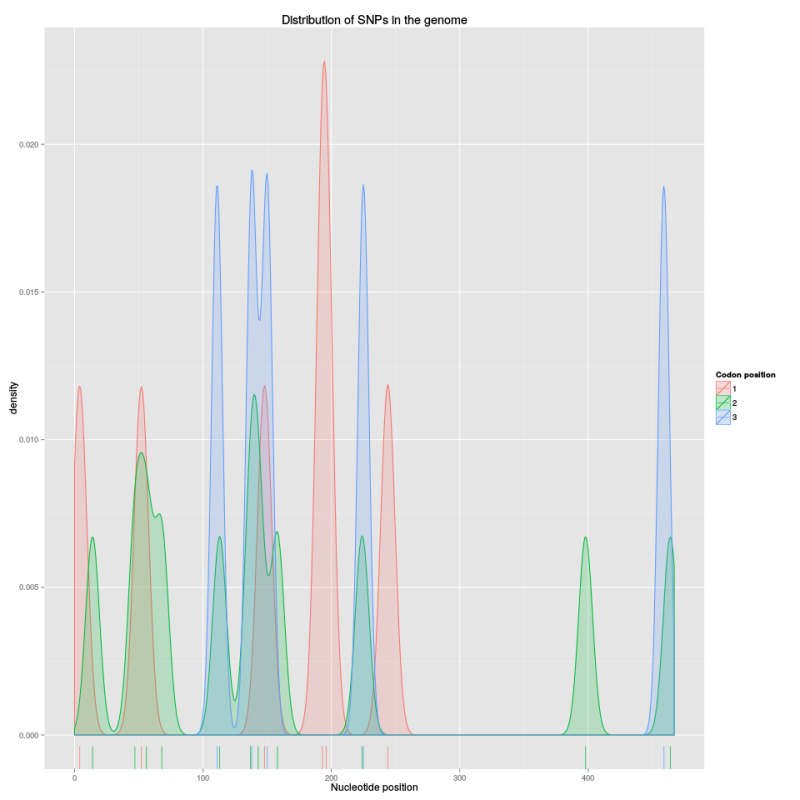
\includegraphics[height=6cm]{snpposi.png}
  \end{flushright}
\end{multicols}
\end{frame}

\begin{frame}[fragile]{Checking sequences}
  \begin{spluscode}
    # Nucleotide diversity
    pegas::nuc.div(x=meles.dna)
    # Base frequencies
    ape::base.freq(x=meles.dna)
    # GC content
    ape::GC.content(x=meles.dna)
    # Number of times any dimer/trimer/etc oligomers occur in a sequence
    # Note: count() requires single sequence as DNAbin/character
    seqinr::count(seq=meles.nogaps[["KJ161328.1"]], wordsize=3)
    # View sequences - all must be of the same length
    image(x=usflu.dna, c("a", "t", "c" ,"g", "n"), col=rainbow(5))
    # Function "image" requires as input matrix
    # So that sequences must be of same length
    image(x=as.matrix(meles.dna), c("a", "t", "c" ,"g", "n"),
      col=rainbow(5))
    # Direct function to display the sequences
    image.DNAbin(x=usflu.dna)
    image.DNAbin(x=as.matrix(meles.dna))
  \end{spluscode}
\end{frame}

\begin{frame}{\textit{Meles} sequences}
  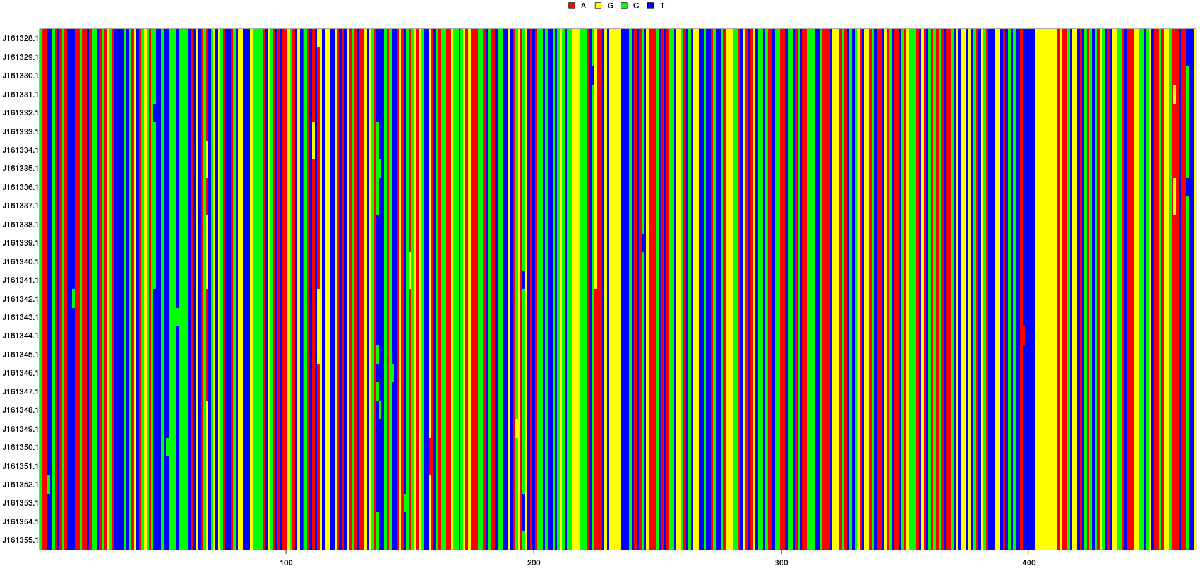
\includegraphics[width=\textwidth]{sequences_meles.png}
\end{frame}

\begin{frame}{Notes about using genlight (vs. genind)}
  \begin{itemize}
    \item Genlight is ``just'' version of more common genind object to store large data sets with (nearly) complete multiple genomes
    \item ``Large'' is tricky -- there is no easy criterion (roughly, genind is inefficient since dozens or hundreds thousands of SNPs) -- try genind and when work fails because of not enough computer resources, go on with genlight
    \item Use is basically same as when working with genind -- but not all functions are able to deal with it (on the other hand, others are optimized to work well on large data sets)
    \item SNPbin is version of genind/genlight to store one large genome -- serves basically as storage, no need to deal with it
    \item Genlight as well as genind allow varying ploidy level
    \item Functions working with genlight use to use parallelisation to speed up operations -- this commonly doesn't work properly on MS~Windows
  \end{itemize}
\end{frame}

\subsection{Export}

\begin{frame}[fragile]{Export data}
  \begin{spluscode}
    # Convert genind into DF using genind2df()
    hauss.df <- genind2df(x=hauss.genind, pop=NULL, sep="/",
      usepop=TRUE, oneColPerAll=FALSE)
    write.table(x=hauss.df, file="haussdata.txt", quote=FALSE,
      sep="\t", na="NA", dec=".", row.names=TRUE, col.names=TRUE)
    # Export of DNA sequences into FASTA format
    write.dna(x=usflu.dna, file="usflu.fasta", format="fasta",
      append=FALSE, nbcol=6)
    write.fasta(sequences=meles.dna, names=names(meles.dna),
      file.out="meles.fasta", open="w")
    # Export DNA sequnces as NEXUS
    write.nexus.data(x=meles.dna, file="meles.nexus", format="dna")
    # Export trees (objects of class phylo)
    # Writes tree(s) in NEWICK format
    write.tree(phy=hauss.nj.bruvo, file="haussknechtii.nwk")
    # Writes tree(s) in NEXUS format
    write.nexus(hauss.nj.bruvo, file="haussknechtii.nexus")
  \end{spluscode}
\end{frame}

\section{Basic analysis}

\begin{frame}[allowframebreaks]{Introductory overview of statistics and methods}
  \begin{itemize}
    \item \alert{Selected method depends on data type, question to answer,~\ldots}
    \begin{itemize}
      \item Check assumptions and requirements of the methods before usage
      \item Think if the method answers your question
    \end{itemize}
    \item \textbf{Population-genetic indices} -- from slide~\ref{popgenindx}
    \begin{itemize}
      \item Huge number\ldots
      \item Characterize differences among individuals/groups or genetic variability on various levels (within/among individuals/populations,~\ldots)
      \item One number tries to describe whole situation -- always very rough
      \item Description of heterozygosity, allelic richness, distribution of multi locus genotypes among populations, level of inbreeding,~\ldots
    \end{itemize}
    \item \textbf{Distance-based methods} -- from slide~\ref{distances}
    \begin{itemize}
      \item \alert{It is crucial to select appropriate distance method for given data}
      \item Usually require the distance matrix to be Euclidean
      \item Distance matrix has one single number (index) for each pair of comparisons (individuals, populations) -- rough
      \item Generally, the matrices describe pairwise similarities among the individuals/populations
      \item Distance-based methods are phenetic
      \begin{itemize}
	\item Based on similarity (described by the matrix), not on any (evolutionary) model
	\item The matrix based on genetic data is supposed to well reflect the genetic similarity, thus real relationships among individuals/populations
      \end{itemize}
      \item \textbf{Hierarchical clustering} -- from slide~\ref{hierclust}
      \begin{itemize}
	\item Several methods clustering individuals according to their (dis)similarity from top or down into clusters
	\item (Un)weighted per-group mean average (\textbf{U/WPGMA}) and others
	\item Used more in ecology, in genetic data not so much anymore (following methods use to produce better results)
      \end{itemize}
      \item \textbf{Neighbor-Joining (NJ)} -- from slide~\ref{NJ}
      \begin{itemize}
	\item A tree starting from the two most similar individuals and connecting in the next steps next and next the most similar individual
	\item In some cases artificially chains individuals
	\item Several methods try to improve it -- slide~\ref{NJ-replacement}
      \end{itemize}
      \item \textbf{Principal Coordinates Analysis (PCoA)} -- from slide~\ref{pcoa}
      \begin{itemize}
	\item The most common method of multivariate statistics for genetic data
	\item Shows individuals in 2D scatter plot to retain maximum variability (by finding correlations among loci)
      \end{itemize}
    \end{itemize}
    \item \textbf{Minimum Spanning Network (MSN)} -- slide~\ref{MSN}
    \begin{itemize}
      \item Simple network connecting the most similar genotypes/haplotypes
      \item Useful for clones, cpDNA, mtDNA,~\ldots
      \end{itemize}
    \item \textbf{Multivariate statistics}
    \begin{itemize}
      \item Two variables are easily displayable in 2D xy-scatter plot (we can calculate correlation, whatever)
      \item In molecular data, each locus is more or less independent variable -- 1000~bp alignment has 1000 variables: How to display plot with 1000 axes to be able to really see something?
      \item Methods like Principal Component Analysis (\textbf{PCA}), Non-Metric Multidimensional Scaling (\textbf{NMDS}) or \textbf{PCoA} look for correlations between pairs of variables to reduce them into new variables -- after many steps new uncorrelated variables retaining maximum of original variability are constructed
      \item New variables are sorted according amount of variability they show (the decrease is very steep -- first 1-4~axes are usually enough) -- it is possible to display xy-scatter plot showing most of variability of the data
      \item Good for data display and creation of hypotheses -- not to verify them (there is no statistical test)
      \item Data are commonly scaled -- all variables are in same scale
    \end{itemize}
    \item \textbf{Maximum Parsimony (MP)} -- from slide~\ref{MP}
    \begin{itemize}
      \item Generally, the methods are looking for the most simple solution under given model, e.g. to construct phylogenetic tree requiring the lowest number of changes
      \item It is easy to score how good the solution is, but computationally demanding to find it
    \end{itemize}
    \item \textbf{Maximum Likelihood (ML)}
    \begin{itemize}
      \item Methods look for the most likely (probable) solution of the data under given model, e.g. the most likely tree under given mutational model
      \item It is easy to score how good the solution is, but computationally demanding to find it
    \end{itemize}
    \item \textbf{Bayesian statistics}
    \begin{itemize}
      \item Based on Bayesian theorem -- probability of model under given data
      \item Methods are looking for the best (e.g. evolutionary) \textbf{model} (e.g. phylogenetic tree) \textbf{explainig the data} (e.g. DNA sequences)
      \item Algorithm exploring possible models and approaching the best runs in steps (generations)
      \begin{itemize}
	\item After some time it converges to find optimal solution (usually described by logarithms of likelihood of given model)
	\item Usually, $\sim$millions (or even more) of generations are required
	\item Beginning use to be very unstable -- it is discarded as burn-in (``heating'' of Markov Chain Monte Carlo (MCMC) doing the exploration and optimization of models), usually $\sim$10-25\%~of steps
      \end{itemize}
    \end{itemize}
    \item MP, ML and Bayesian statistics contain (evolutionary) \textbf{models} -- they are not based on similarity (as matrix-based methods), so that they are supposed to reveal real structure in the data
    \item \textbf{Permutations}, \textbf{bootstraps} and another tests
    \begin{itemize}
      \item It is necessary to test statistical significance of the obtained results
      \item Most common methods somehow shuffle the data (drop one column,~\ldots) and repeat the calculation to see how stable is the result (it might be driven by one or few loci,~\ldots)
      \item Whole process is repeated $\sim$100-1000~times and output is shown as histogram of simulations vs. the observed value, in how many percents the same result was obtained (e.g. bootstrap) or as p-value (what is probability that the pattern was created by random process)
      \item p = 0.05 means 95\% probability that the data are non-random
    \end{itemize}
  \end{itemize}
\end{frame}
  
\subsection{First look at the data}

\begin{frame}[fragile]{Descriptive statistics I}
  \label{popgenindx}
  \begin{itemize}
    \item We will now work mainly with diploid SSRs for \textit{Taraxacum haussknechtii}, you can try other data examples by yourselves
  \end{itemize}
  \begin{spluscode}
    # Get summary - names and sizes of populations,
    # heterozygosity, some info about loci
    hauss.summ <- summary(hauss.genind)
    # Plot expected vs. observed heterozygosity
    # it looks like big difference
    plot(x=hauss.summ$Hexp, y=hauss.summ$Hobs,
      main="Observed vs expected heterozygosity",
      xlab="Expected heterozygosity", ylab="Observed heterozygosity")
    abline(0, 1, col="red")
    # Bartlett's K-squared of difference
    # between observed and expected heterozygosity - not significant
    bartlett.test(list(hauss.summ$Hexp, hauss.summ$Hobs))
                  Bartlett test of homogeneity of variances
    data:  list(hauss.summ$Hexp, hauss.summ$Hobs)
    Bartlett's K-squared = 0.069894, df = 1, p-value = 0.7915
  \end{spluscode}
\end{frame}

\begin{frame}[fragile]{Descriptive statistics II}
  \begin{itemize}
    \item \texttt{t-test} and \texttt{bartlett.test} require data to have normal distribution -- if the condition is not met, it is necessary to use some weaker non-parametric test (\texttt{kruskal.test}, \texttt{wilcox.test},~\ldots)
    \item See respective manual pages for details
    \item \texttt{shapiro.test()} tests the normality of given vector
  \end{itemize}
  \begin{spluscode}
    # T-test of difference between
    # observed and expected heterozygosity - strongly significant
    t.test(x=hauss.summ$Hexp, y=hauss.summ$Hobs, paired=TRUE, var.equal=T)
                 Paired t-test
    data:  hauss.summ$Hexp and hauss.summ$Hobs
    t = 3.5622, df = 11, p-value = 0.004456
    alternative hypothesis: true difference in means is not equal to 0
    95 percent confidence interval:
     0.06114303 0.25887357
    sample estimates:
    mean of the differences
                  0.1600083
  \end{spluscode}
\end{frame}

\begin{frame}[fragile]{Descriptive statistics III}
  \begin{spluscode}
    # Create pane with some information
    par(mfrow=c(2,2)) # Divide graphical devices into 4 smaller spaces
    # Plot alleles number vs. population sizes
    plot(x=hauss.summ$n.by.pop, y=hauss.summ$pop.nall, xlab="Populations
      sample size", ylab="Number of alleles", main="Alleles numbers and
      sample sizes", col="red", pch=20)
    # Add text description to the point
    text(x=hauss.summ$n.by.pop, y=hauss.summ$pop.nall,
      lab=names(hauss.summ$n.by.pop), cex=1.5)
    # Barplots of various data
    barplot(height=hauss.summ$loc.n.all, ylab="Number of alleles",
      main="Number of alleles per locus", las=3)
    barplot(height=hauss.summ$Hexp-hauss.summ$Hobs, main="Heterozygosity:
      expected-observed", ylab="Hexp - Hobs", las=3)
    barplot(height=hauss.summ[["n.by.pop"]], main="Sample sizes per
      population", ylab="Number of genotypes", las=3)
    dev.off() # Closes graphical device - otherwise following
              # graphs would still be divided into 4 parts
  \end{spluscode}
\end{frame}

\begin{frame}{Graphs from previous slides}
  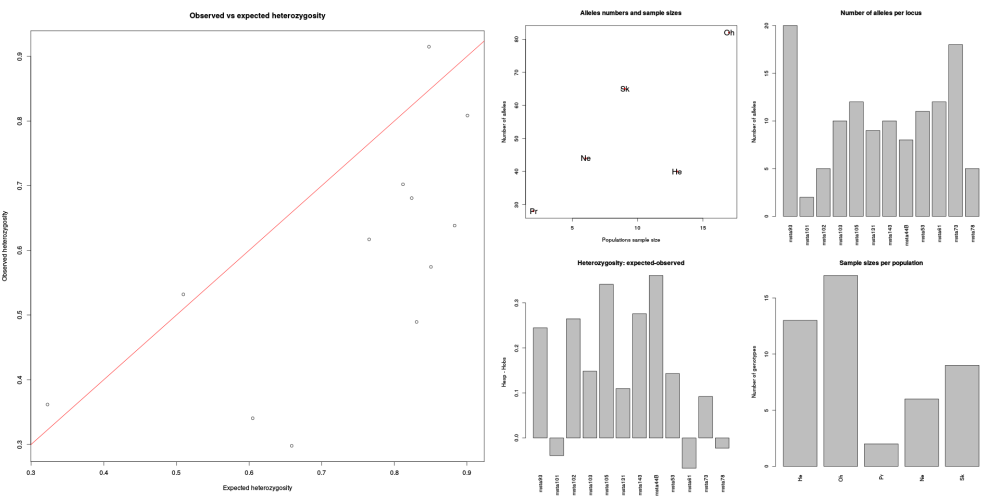
\includegraphics[width=\textwidth]{heterozygosity.png}
\end{frame}

\subsection{Statistics}

\begin{frame}[fragile]{Population statistics by poppr()}
  \vfill
  \begin{itemize}
    \item \texttt{poppr()} is central function of \texttt{poppr} package calculating plenty of population genetic indices
  \end{itemize}
  \vfill
  \begin{spluscode}
    ?poppr # See details
    poppr(dat=hauss.genind, total=TRUE, sample=1000, method=4,
      missing="geno", cutoff=0.15, quiet=FALSE, clonecorrect=FALSE,
      plot=TRUE, index="rbarD", minsamp=1, legend=TRUE)
    ... # Output table with indices:
      Pop  N MLG eMLG       SE     H     G lambda   E.5  Hexp   Ia # More...
       He 13  11 1.97 1.58e-01 2.352  9.94  0.899 0.941 0.503 1.42 ...
       Ne  6   5 1.93 2.49e-01 1.561  4.50  0.778 0.930 0.604 3.44 ...
      ...... ...  ...      ...   ...   ...    ...   ...   ...  ... ...
    Total 47  43 2.00 6.07e-02 3.732 40.16  0.975 0.961 0.742 1.88 ...
  \end{spluscode}
  \vfill
  \begin{itemize}
    \item If \texttt{plot=TRUE}, histogram of simulations (\texttt{sample} must be > 1) is plotted for each population for \texttt{rbarD} or \texttt{Ia} (according to selected \texttt{index} -- see following slides for details)
  \end{itemize}
  \vfill
\end{frame}

\begin{frame}{Histograms of simulations of rbarD for each population}{The populations are significantly far from being clonal}
  \begin{center}
    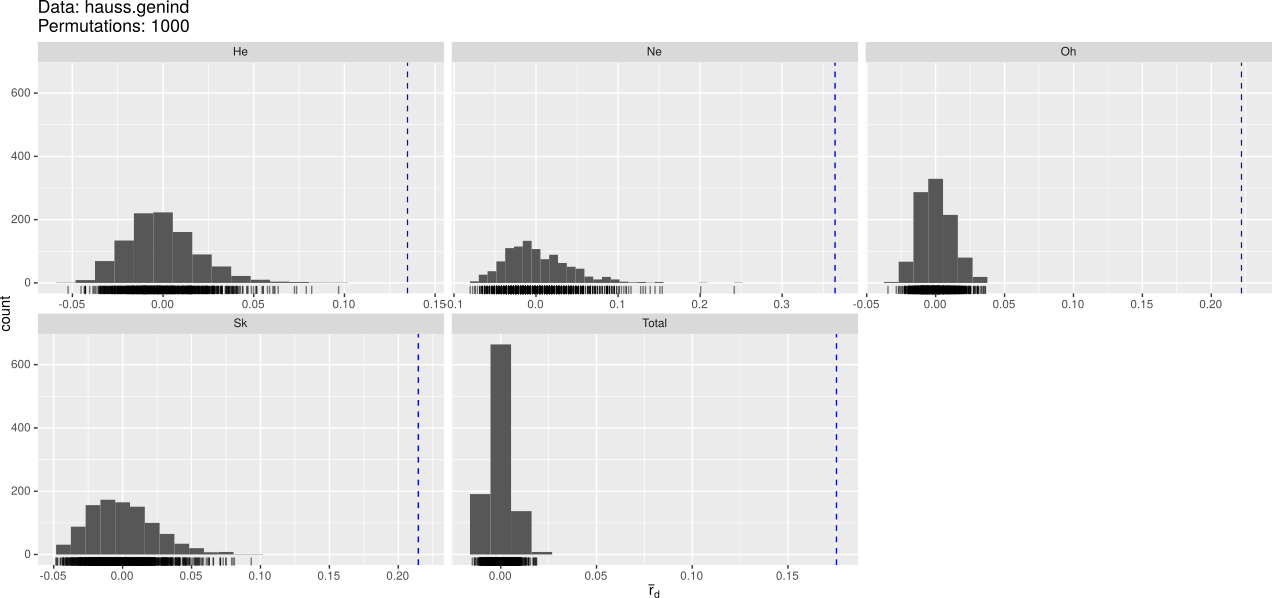
\includegraphics[height=6.5cm]{poppr.png}
  \end{center}
\end{frame}

\begin{frame}[allowframebreaks]{Population statistics returned by poppr()}
  \begin{block}{Too much to choose from?}
    Generally, there are plenty of different population indices (and distances and another statistics) with different assumptions and usage in many packages -- it can be complicated to pick the best one\ldots{ }The course shows many examples, but the list is far from being exhaustive\ldots
  \end{block}
  \begin{itemize}
    \item \texttt{Pop} -- Population analyzed
    \begin{itemize}
      \item If \texttt{total=TRUE}, there are also statistics for whole dataset
    \end{itemize}
    \item \texttt{N} -- Number of individuals/isolates in the specified population
    \item \texttt{MLG} -- Number of multilocus genotypes found in the specified population (see \texttt{?mlg})
    \item \texttt{eMLG} -- The expected number of MLG at the lowest common sample size (set by \texttt{minsamp})
    \item \texttt{SE} -- The standard error for the rarefaction analysis (assets species richness -- how it grows with growing sample size)
    \begin{itemize}
      \item Big difference between \texttt{MLG} and \texttt{eMLG} indicate some process lowering/increasing genetic diversity
    \end{itemize}
    \item \texttt{H} -- \href{https://en.wikipedia.org/wiki/Diversity_index\#Shannon_index}{Shannon-Wiener Diversity index} -- evaluates number of genotypes and their distribution, takes entropy into account, grows with higher richness and diversity, sensitive to uneven sample size
    \item \texttt{G} -- \href{http://www.genetics.org/content/118/4/705}{Stoddard and Taylor's Index} -- roughly, similar approach as the previous one, highly enhanced
    \item \texttt{lambda} -- \href{https://en.wikipedia.org/wiki/Diversity_index\#Simpson_index}{Simpson's index} $\lambda$ = 1 minus the sum of squared genotype frequencies -- estimation of the probability that two randomly selected genotypes are different and scales from 0 (no genotypes are different) to 1 (all genotypes are different)
    \item \texttt{E.5} -- Evenness -- measure of the distribution of genotype abundances, wherein a population with equally abundant genotypes yields a value equal to 1 and a population dominated by a single genotype is closer to 0
    \item \texttt{Hexp} -- \href{http://www.genetics.org/content/89/3/583}{Nei's gene diversity} (expected heterozygosity) -- unbiased gene diversity (from 0 = no diversity to 1 = highest diversity)
    \item \texttt{Ia} -- Index of Association (\texttt{?ia}) -- widely used to detect clonal reproduction within populations
    \begin{itemize}
      \item Populations whose members are undergoing sexual reproduction will produce gametes via meiosis, and thus have a chance to shuffle alleles in the next generation
      \item Populations whose members are undergoing clonal reproduction generally do so via mitosis -- most likely mechanism for a change in genotype is via mutation -- the rate of mutation varies from species to species, but it is rarely sufficiently high to approximate a random shuffling of alleles
      \item The index of association is a calculation based on the ratio of the variance of the raw number of differences between individuals and the sum of those variances over each locus
      \item It as the observed variance over the expected variance -- if they are the same, then the index is zero (=prevailing clonal reproduction) after subtracting one -- it rises with with increasing differences
    \end{itemize}
    \item \texttt{p.Ia} -- P-value for \texttt{Ia} from the number of reshuffling indicated in \texttt{sample}
    \item \texttt{rbarD} -- Standardized Index of Association for each population (see \texttt{?ia}) -- corrected for higher number of loci not to rise so steeply
    \item \texttt{p.rD} -- P-value for \texttt{rbarD} from the number of reshuffles indicated in \texttt{sample}
    \item See \href{https://grunwaldlab.github.io/Population_Genetics_in_R/index.html}{poppr's manual} and \texttt{vignette("algo", package="poppr")} for details
  \end{itemize}
\end{frame}

\begin{frame}[fragile]{Departure from Hardy-Weinberg equilibrium}
  \begin{itemize}
    \item \href{https://en.wikipedia.org/wiki/Hardy%E2%80%93Weinberg_principle}{In theory}, in large panmictic population without evolutionary influence everyone can mate with everyone (it is in equilibrium) and allele frequencies remain stable -- in reality, environment, behavior, mutations, genetic drift, etc. are structuring the population
  \end{itemize}
  \begin{spluscode}
    # According to loci
    hauss.hwe.test <- hw.test(x=hauss.loci, B=1000)
    hauss.hwe.test
    # According to populations
    # Separate genind object into list of genind objects for individual
    # populations
    hauss.pops <- seppop(hauss.genind)
    hauss.pops
    # Convert genind back to loci (list of loci objects according to
    # populations)
    hauss.pops.loci <- lapply(X=hauss.pops, FUN=genind2loci)
    # Calculate the results per populations
    lapply(X=hauss.pops.loci, FUN=hw.test, B=1000)
  \end{spluscode}
\end{frame}

\begin{frame}[fragile]{Departure from HWE -- results per locus}
  \vfill
  \splus/hauss.hwe.test/
  \begin{tabular}{lllll}
    & chi\textasciicircum2 & df & Pr(chi\textasciicircum2 >) & Pr.exact\\
    msta93 & 383.5519728 & 190 & 3.552714e-15 & 0.000\\
    msta101 & 0.6927242 & 1 & 4.052393e-01 & 0.657\\
    msta102 & 83.0741964 & 10 & 1.250111e-13 & 0.000\\
    msta103 & 77.1819098 & 45 & 1.998865e-03 & 0.000\\
    ... & ... & ... & ... & ...
  \end{tabular}
  \vfill
  \begin{itemize}
    \item Pr.exact shows significance of the departure (i.e. non-equilibrial distribution of alleles within population -- calculated per loci)
    \item $\chi^2$ \href{https://en.wikipedia.org/wiki/Pearson%27s_chi-squared_test}{test} (without or with the permutations) test the departure -- if it is significant or not -- not how much it is departing
  \end{itemize}
  \vfill
\end{frame}

\begin{frame}[fragile]{F-statistics I}
  \begin{itemize}
    \item Functions return tables of F-statistics values for populations/loci (roughly 0 -- no structure, 1 -- fully structured)
    \item The different \href{https://en.wikipedia.org/wiki/F-statistics}{F-statistics} look at different levels of population structure. F$_{IT}$ is the inbreeding coefficient of an individual relative to the total population; F$_{IS}$ is the inbreeding coefficient of an individual relative to the subpopulation and averaging them; and F$_{ST}$ is the effect of subpopulations compared to the total population
    \item For \texttt{Fst}, \texttt{fstat} and \texttt{theta.msat} the loci object \textbf{must} contain population column
  \end{itemize}
  \begin{spluscode}
    # Fit, Fst and Fis for each locus
    Fst(x=hauss.loci, pop=1)
                    Fit        Fst         Fis
    msta93   0.31835291 0.17867087  0.17006829
    msta101 -0.09968472 0.04064928 -0.14628018
        ...         ...        ...         ...
  \end{spluscode}
\end{frame}

\begin{frame}[fragile]{F-statistics II}
  \begin{spluscode}
    # Multilocus estimators of variance components and F-statistics,
    # alternative to Fst
    library(hierfstat)
    fstat(x=hauss.genind, pop=NULL, fstonly=FALSE)
                pop       Ind
    Total 0.1589501 0.2582641
    pop   0.0000000 0.1180834
    # Nei's pairwise Fst between all pairs of populations.
    # 0 = no structure; 1 = maximal difference
    pairwise.fst(x=hauss.genind, pop=NULL, res.type="matrix")
               He         Ne         Oh         Pr         Sk
    He 0.00000000 0.19960826 0.11391904 0.09404571 0.11184561
    Ne 0.19960826 0.00000000 0.07265306 0.19220430 0.10112859
    Oh 0.11391904 0.07265306 0.00000000 0.05302854 0.06287497
    Pr 0.09404571 0.19220430 0.05302854 0.00000000 0.10436469
    Sk 0.11184561 0.10112859 0.06287497 0.10436469 0.00000000
  \end{spluscode}
\end{frame}

% TODO population theta
%     # Estimates of population theta according to Kimmel et al. 1998
%     theta.msat(hauss.loci)
%                theta.v    theta.h theta.x
%     msta93  1287.09037 42.7450000  49.500
%     msta101  105.62800  0.6006928   0.000
%         ...        ...        ...     ...

\begin{frame}[fragile]{Multi locus genotypes}
  \begin{multicols}{2}
  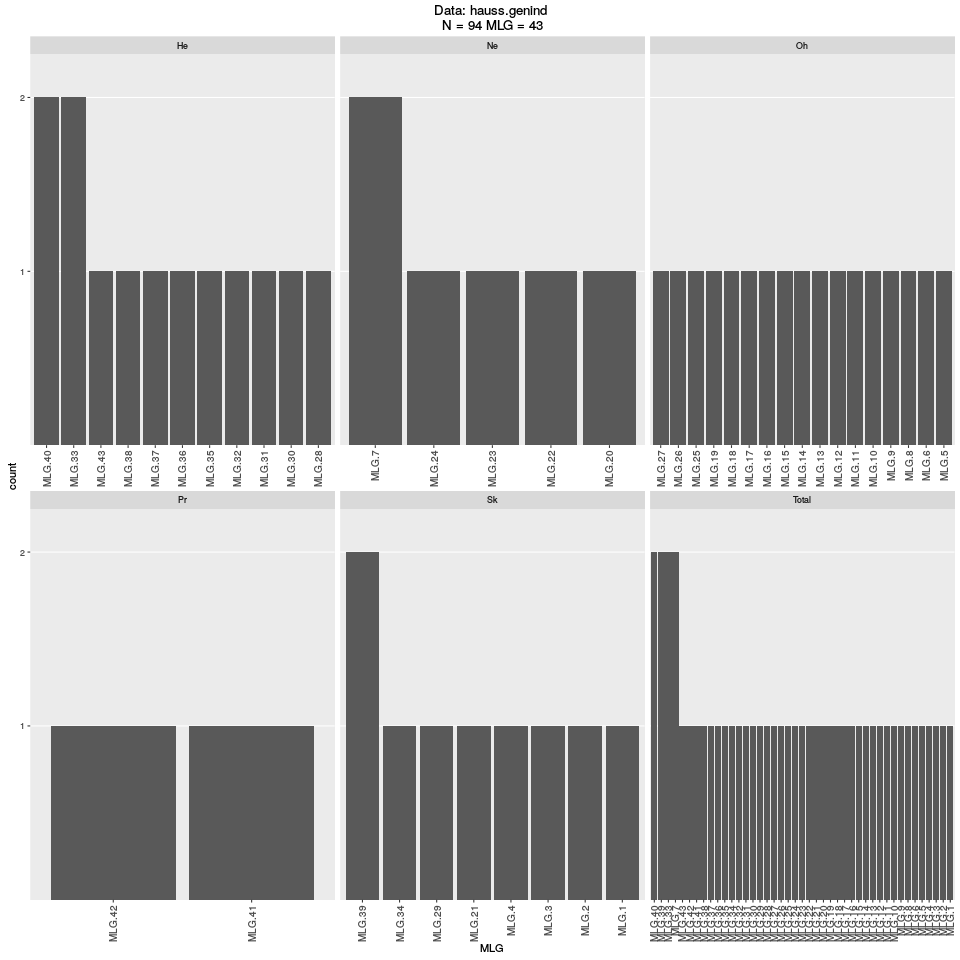
\includegraphics[height=5.5cm]{mlg.png}
  \begin{spluscode}
    # Total number of MLGs
    # (simple value)
    mlg(gid=hauss.genind, quiet=FALSE)
    # MLGs shared among populations
    mlg.crosspop(gid=hauss.genind,
      df=TRUE, quiet=FALSE)
    # Detailed view on distribution
    # of MLGs into populations
    # (table and/or plot)
    mlg.table(gid=hauss.genind,
      bar=TRUE, total=TRUE,
      quiet=FALSE)
    mlg.vector(hauss.genind)
    mlg.id(hauss.genind)
  \end{spluscode}
  \end{multicols}
  Functions from poppr package -- the best for microsatellites, although available also from another data types
\end{frame}

\begin{frame}[fragile]{Inbreeding}
\begin{multicols}{2}
  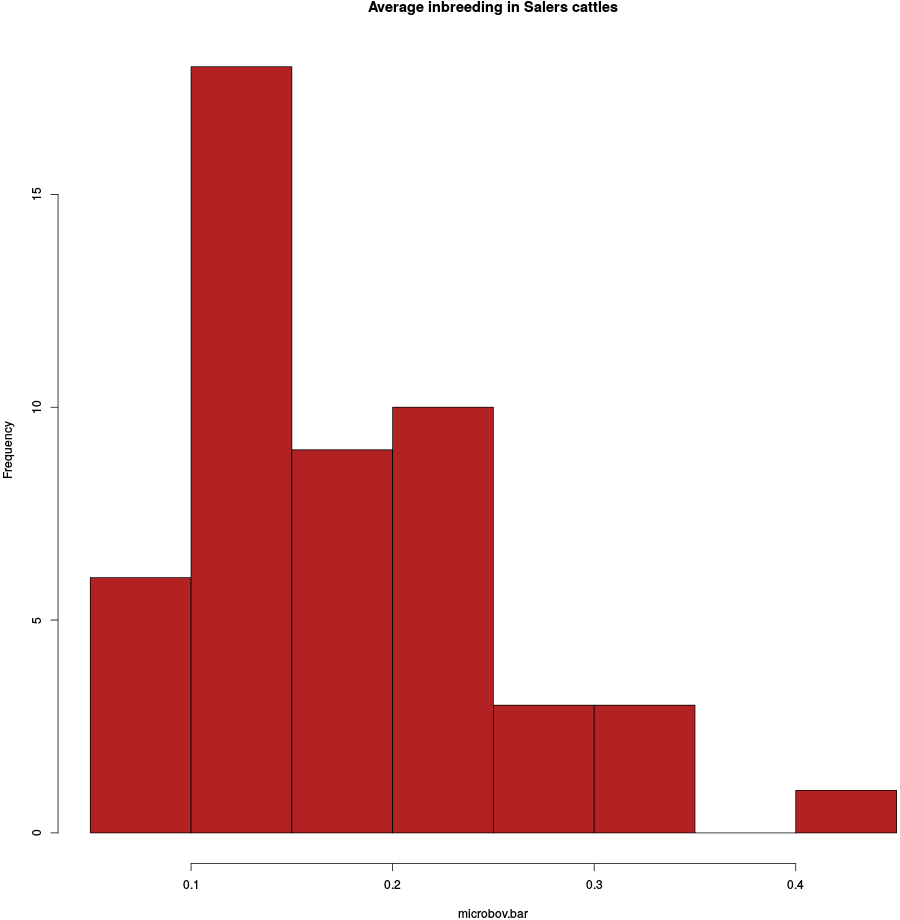
\includegraphics[height=5.5cm]{inbreeding.png}
  \begin{spluscode}
    # Load training data (cattle)
    data(microbov)
    # Separate populations of Salers
    microbov.pops <- seppop(microbov)
      [["Salers"]]
    # Calculate the inbreeding
    microbov.inbr <- inbreeding(x=
      microbov.pops, N=100)
    # Check for more settings
    ?inbreeding
    # population means for plotting
    microbov.bar <- sapply(X=
      microbov.inbr, FUN=mean)
    # Plot it
    hist(x=microbov.bar, col=
      "firebrick", main="Average
      inbreeding in Salers cattles")
  \end{spluscode}
\end{multicols}

\end{frame}

\subsection{Genetic distances}

\begin{frame}[fragile]{Basic distances}
  \label{distances}
  \begin{spluscode}
    # See ?dist.gene for details about methods of this distance
    hauss.dist.g <- dist.gene(x=hauss.genind@tab, method="pairwise")
    # Euclidean distance for individuals (plain ordinary distance matrix)
    hauss.dist <- dist(x=hauss.genind, method="euclidean", diag=T, upper=T)
    hauss.dist
    # Nei's distance (not Euclidean) for populations
    # (other methods are available, see ?dist.genpop)
    hauss.dist.pop <- dist.genpop(x=hauss.genpop, method=1, diag=T, upper=T)
    # Test if it is Euclidean
    is.euclid(hauss.dist.pop, plot=TRUE, print=TRUE, tol=1e-10) # FALSE = No
    # Turn to be Euclidean
    hauss.dist.pop <- cailliez(distmat=hauss.dist.pop, print=FALSE,
      tol=1e-07, cor.zero=TRUE)
    # Test if it is Euclidean
    is.euclid(hauss.dist.pop, plot=TRUE, print=TRUE, tol=1e-10) # TRUE = OK
  \end{spluscode}
  \vfil
  Most of analysis based on distances more or less require \href{https://en.wikipedia.org/wiki/Euclidean_distance_matrix}{Euclidean distances} (non-negative, Pythagoeran theorem is valid, etc.). If the distance matrix contains non-Euclidean distances, the result can be weird\ldots
  \vfill
\end{frame}

\begin{frame}[fragile]{Distances reflecting microsatellite repeats}
  \begin{spluscode}
    # Bruvo's distances weighting SSRs repeats - take care about replen
    # parameter - requires repetition length for every SSRs locus
    hauss.dist.bruvo <- bruvo.dist(pop=hauss.genind, replen=rep(2, 12),
      loss=TRUE)
    # Test if it is Euclidean
    is.euclid(hauss.dist.bruvo, plot=TRUE, print=TRUE, tol=1e-10)
    # Turn to be Euclidean
    hauss.dist.bruvo <- cailliez(distmat=hauss.dist.bruvo, print=FALSE,
      tol=1e-07, cor.zero=TRUE)
    # Test if it is Euclidean
    is.euclid(hauss.dist.bruvo, plot=TRUE, print=TRUE, tol=1e-10)
    # Show it
    hauss.dist.bruvo
  \end{spluscode}
  \begin{itemize}
    \item See poppr's manual and manual pages of the functions for details and different possibilities of settings
    \item Be careful when changing non-Euclidean distances to Euclidean -- \alert{the transformation more or less changes meaning of the distances!}
  \end{itemize}
\end{frame}

\begin{frame}{Turning distance matrix into Euclidean is controversial\ldots}
  \begin{footnotesize}
    How to deal with zero distances in original matrix? There is no really good solution\ldots\\ Histograms of Bruvo distance before and after transformation:
  \end{footnotesize}
  \begin{center}
    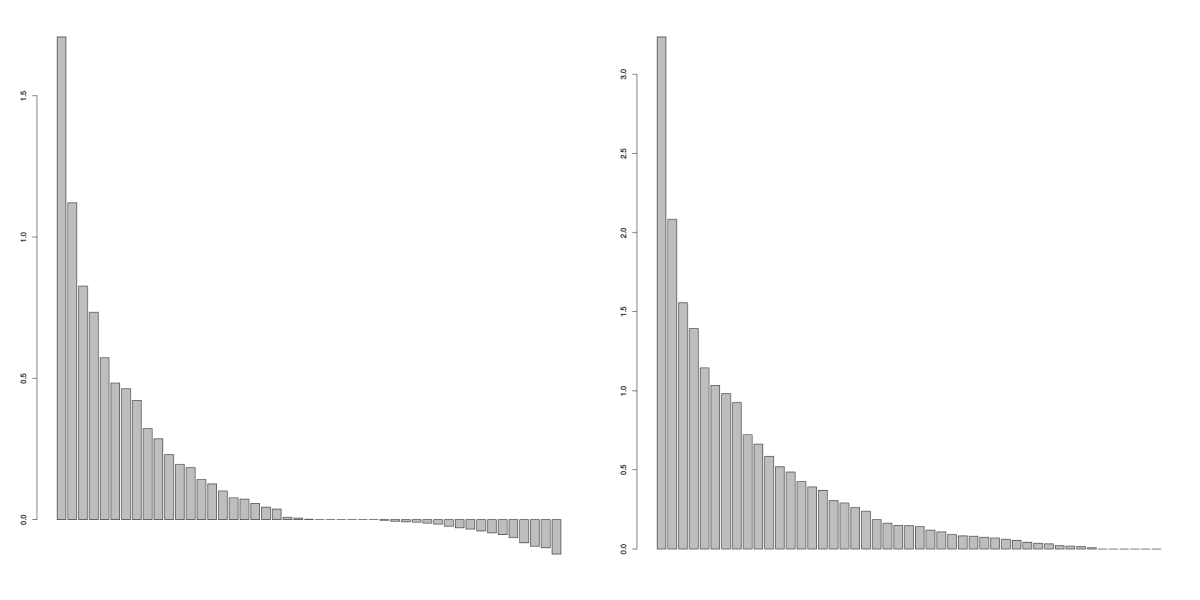
\includegraphics[width=\textwidth]{bruvodist.png}
  \end{center}
\end{frame}

\begin{frame}[fragile]{More distances\ldots}
  \begin{spluscode}
    # Nei's distance (not Euclidean) for individuals
    # (other methods are available, see ?nei.dist from poppr package)
    hauss.dist.nei <- nei.dist(x=hauss.genind, warning=TRUE)
    hauss.dist.nei
    # Dissimilarity matrix returns a distance reflecting the number of
    # allelic differences between two individuals
    hauss.dist.diss <- diss.dist(x=hauss.genind, percent=FALSE, mat=TRUE)
    hauss.dist.diss
  \end{spluscode}
\vfill
\textbf{Import own distance matrix from another software:}
\begin{multicols}{2}
  \begin{spluscode}
       Fe       He      Oh      ...
    Fe 0.00000  132.019 109.159 ...
    He 132.0191 0.00000 9.89111 ...
    Oh 109.1590 9.89111 0.00000 ...
    Pr 139.5669 8.55312 4.40562 ...
    Ne 156.7619 9.96143 16.6927 ...
    ... ...     ...     ...     ...
  \end{spluscode}
  \columnbreak
  \begin{spluscode}
    MyDistance <- read.csv("distances.
      txt", header=TRUE, sep="\t",
      dec=".", row.names=1)
    MyDistance <- as.dist(MyDistance)
    class(MyDistance)
    dim(MyDistance)
    MyDistance
  \end{spluscode}
\end{multicols}
\end{frame}

\begin{frame}[fragile]{Different distances have different use case and outputs\ldots}
  \vfill
  \begin{tabular}{llll}
    \textbf{Method} & \textbf{Function} & \textbf{Assumption} & \textbf{Euclidean}\\
    \href{http://link.springer.com/article/10.1007/BF00831894}{Prevosti 1975} & \texttt{prevosti.dist}, & --- & \alert{No}\\
     & \texttt{diss.dist} & & \\
    \href{http://www.jstor.org/stable/2459777}{Nei 1972}, \href{http://www.genetics.org/content/89/3/583.short}{1978} & \texttt{nei.dist} & Infinite Alleles, & \alert{No}\\
     & & Genetic Drift & \\
    \href{http://www.jstor.org/stable/2528824}{Edwards 1971} & \texttt{edwards.dist} & Genetic Drift & Yes\\
    \href{http://www.genetics.org/node/324318.full}{Reynolds 1983} & \texttt{reynolds.dist} & Genetic Drift & Yes\\
    Rogers 1972\footnote{Rogers (1972): Measures of genetic similarity and genetic distances. Pp. 145-153 of Studies in Genetics. University of Texas Publishers} & \texttt{rogers.dist} & --- &\\
    \href{http://onlinelibrary.wiley.com/doi/10.1111/j.1365-294X.2004.02209.x/full}{Bruvo 2004} & \texttt{bruvo.dist} & Stepwise Mutation & \alert{No}
  \end{tabular}
  \vfill
  \begin{spluscode}
    # See details of distance methods in package poppr
    vignette("algo", package="poppr")
  \end{spluscode}
  \vfill
\end{frame}

\begin{frame}[fragile]{Comparison of different matrices}
  \begin{spluscode}
    # Compare different distance matrices
    # List of functions to be parsed to respective dist.* function
    distances <- c("Nei", "Rogers", "Edwards", "Reynolds", "Prevosti")
    # Calculate the distance matrices
    dists <- lapply(distances, function(x) {
      DISTFUN <- match.fun(paste(tolower(x), "dist", sep="."))
      DISTFUN(hauss.genind.cor) })
    # Add names for the distance names
    names(dists) <- distances
    # Add Bruvo distance
    dists[["Bruvo"]] <- hauss.dist.bruvo
    dists
    # Split graphical device into 2 lines, 3 panes each
    par(mfrow=c(2, 3))
    # Calculate NJ and plot all trees
    x <- lapply(names(dists), function(x) {
      plot(njs(dists[[x]]), main=x, type="unrooted")
      add.scale.bar(lcol="red", length=0.1) })
    dev.off() # Close graphical device to reset settings
  \end{spluscode}
\end{frame}

\begin{frame}{Neigbor-Joining of same dataset under different matrices}{The results are very different\ldots}
  \begin{center}
    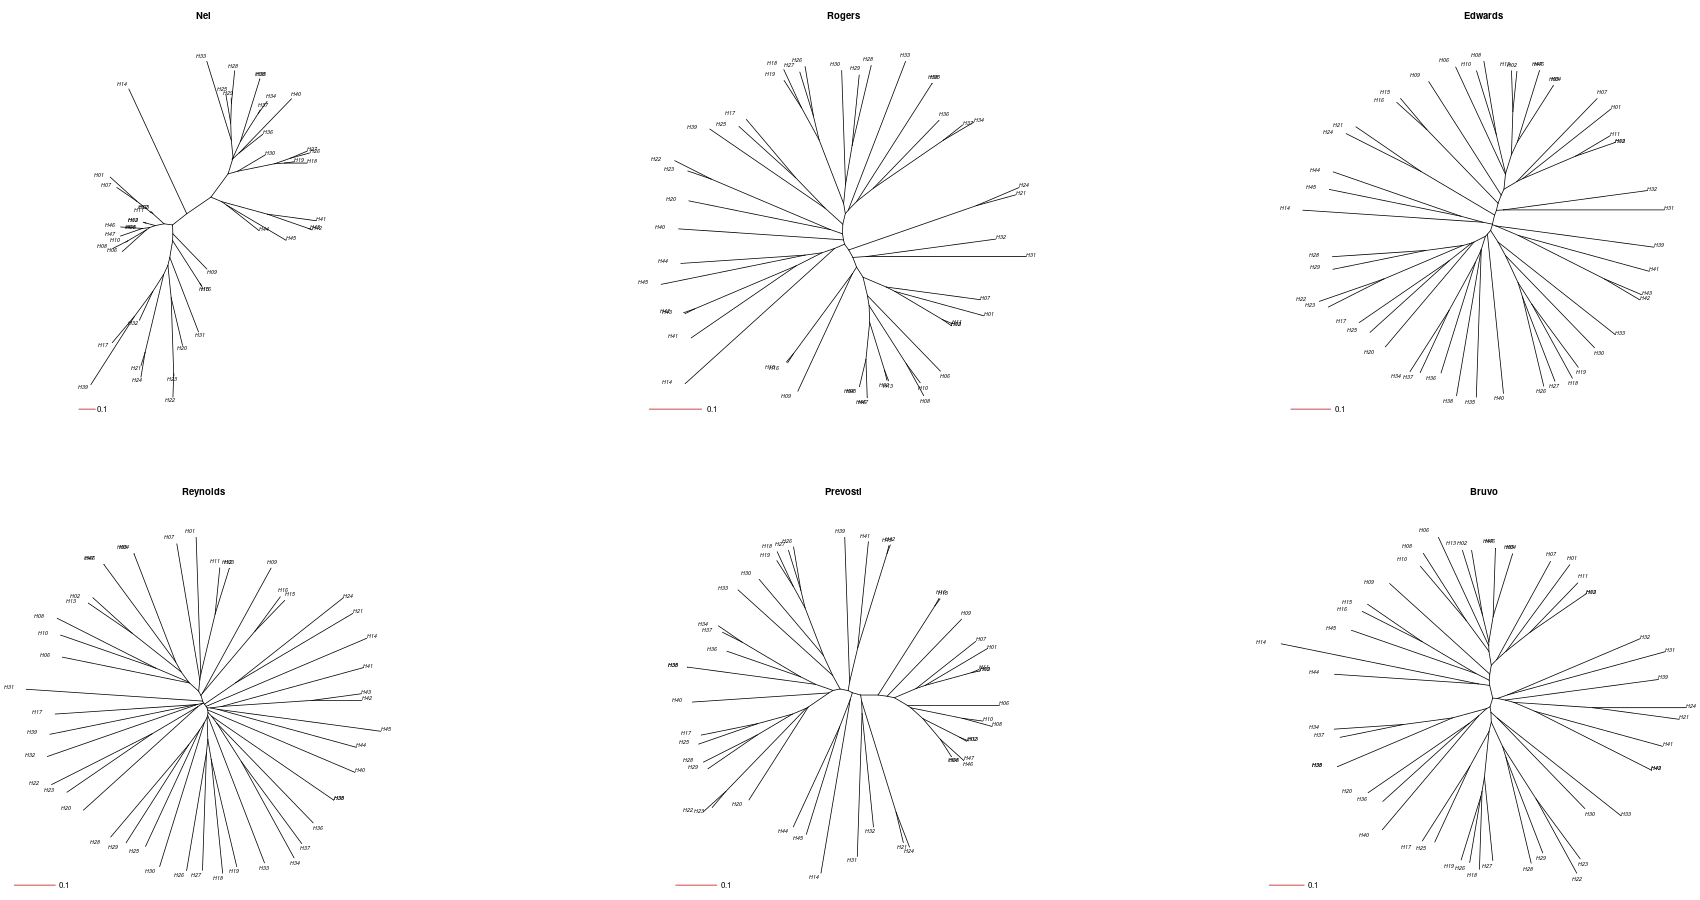
\includegraphics[width=\textwidth]{distances.png}
  \end{center}
\end{frame}

\begin{frame}[fragile]{Distances among DNA sequences}
  \begin{itemize}
    \item \alert{The sequences must be aligned before calculating distances among them!}
    \item Selection of mutational model has significant impact to results\ldots
  \end{itemize}
  \vfill
  \begin{spluscode}
    # There are various models available
    ?dist.dna
    # Create the distance matrix
    usflu.dist <- dist.dna(x=usflu.dna, model="TN93")
    # Check the resulting distance matrix
    usflu.dist
    class(usflu.dist)
    # Create another distance matrix
    dim(as.matrix(usflu.dist))
    # Check it
    meles.dist <- dist.dna(x=meles.dna, model="F81")
    meles.dist
    class(meles.dist)
    dim(as.matrix(meles.dist))
  \end{spluscode}
\end{frame}

\begin{frame}[fragile]{Distances and genlight object}
  \vfill
  Pairwise genetic distances for each data block (genlight objects with whole genome data) -- sensitive to missing data (not useful in every case):
  \vfill
  \begin{spluscode}
    usflu.dists.l <- seploc(usflu.genlight, n.block=10, parallel=FALSE)
    class(usflu.dists.l)
    usflu.dists <- lapply(X=usflu.dists.l, FUN=function(DDD)
      dist(as.matrix(DDD)))
    class(usflu.dists)
    names(usflu.dists)
    class(usflu.dists[[1]])
    usflu.distr <- Reduce(f="+", x=usflu.dists)
    class(usflu.distr)
    usflu.distr
    # It is possible to use just basic dist function on whole
    # genlight object (might require a lot of RAM)
    usflu.distg <- dist(as.matrix(usflu.genlight))
  \end{spluscode}
  \vfil
  Rationale of this approach is to save resources when dividing whole data set into smaller blocks -- useful for huge data, not for all of the cases
  \vfill
\end{frame}

\begin{frame}[fragile]{Visualize pairwise genetic similarities}
\begin{multicols}{2}
\vfil
  \begin{spluscode}
    # table.paint() requires data
    # frame, dist can't be directly
    # converted to DF
    table.paint(df=as.data.frame(
      as.matrix(usflu.dist)), cleg=0,
      clabel.row=0.5, clabel.col=0.5)
    # Same visualization, colored
    # heatmap() reorders values
    # because by default it plots
    # also dendrograms on the edges
    heatmap(x=as.matrix(usflu.dist),
      Rowv=NA, Colv=NA, symm=TRUE)
  \end{spluscode}
\begin{itemize}
 \item Colored according to value
 \item Another possibility is to use \texttt{corrplot::corrplot()} for correlation plots
\end{itemize}
  \columnbreak
  \begin{center}
    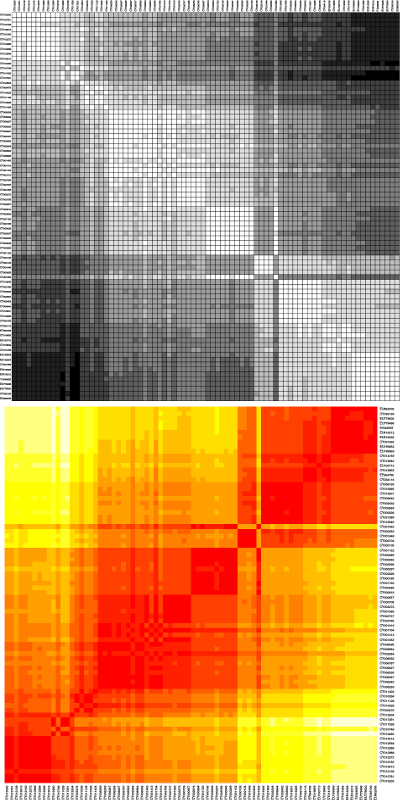
\includegraphics[height=6cm]{dna-dists.png}
  \end{center}
\end{multicols}
\end{frame}

\subsection{Hierarchical clustering}

\begin{frame}[fragile]{Heatmaps}
\label{hierclust}
\begin{multicols}{2}
  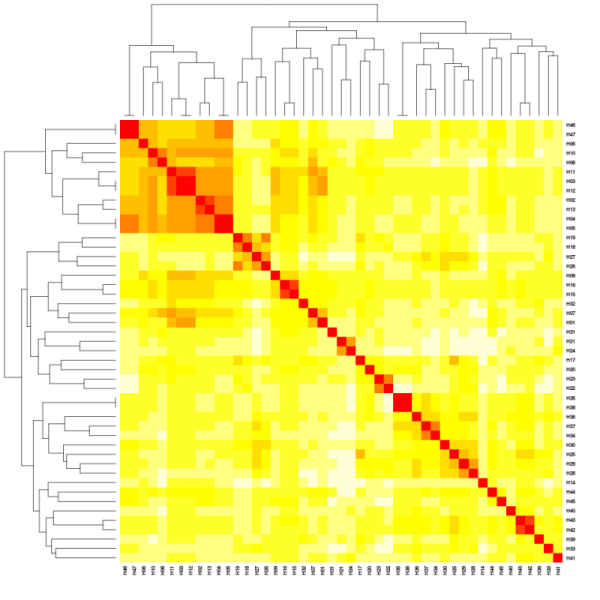
\includegraphics[height=6cm]{heatmap.png}
  \columnbreak
  \begin{spluscode}
    # Based on various distances
    heatmap(as.matrix(hauss.dist),
      symm=TRUE, labRow=rownames(
      as.matrix(hauss.dist.bruvo)),
      labCol=colnames(as.matrix(
      hauss.dist.bruvo)))
      # hauss.dist doesn't contain
      # names of individuals - add here
    heatmap(as.matrix(hauss.dist.pop),
      symm=TRUE)
    heatmap(as.matrix(hauss.dist.
      bruvo), symm=TRUE)
    heatmap(as.matrix(hauss.dist.
      diss), symm=TRUE)
  \end{spluscode}
  \begin{footnotesize}
  There are various settings -- colors, dendrogram,~\ldots See~\texttt{?heatmap}.
  \end{footnotesize}
\end{multicols}
\end{frame}

\begin{frame}[fragile]{Hierarchical clustering -- UPGMA and others}
\begin{multicols}{2}
  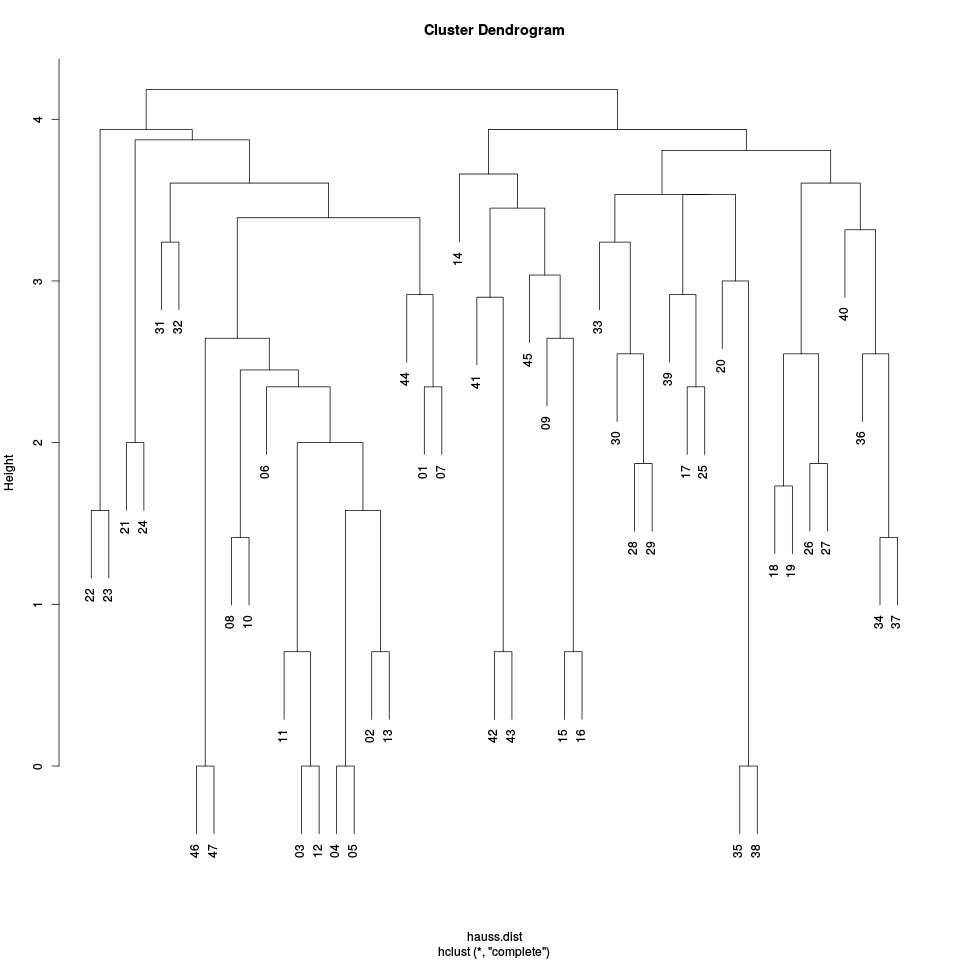
\includegraphics[height=6cm]{hierclust.png}
  \begin{spluscode}
    # According to distance used
    # see ?hclust for methods
    plot(hclust(d=hauss.dist,
      method="complete"))
    plot(hclust(d=hauss.dist.pop,
      method="complete"))
    plot(hclust(d=hauss.dist.
      bruvo, method="complete"))
  \end{spluscode}
  \vfil
  \begin{itemize}
    \item This is very basic function to make dendrogram
    \item There are better possibilities (NJ etc -- see slide \ref{NJ} and onward)
  \end{itemize}
\end{multicols}
\end{frame}

\begin{frame}[fragile]{UPGMA and its test}
  \begin{spluscode}
    # Calculate it
    # Saving as phylo object (and not hclust) gives more
    # possibilities for further plotting and manipulations
    usflu.upgma <- as.phylo(hclust(d=usflu.dist, method="average"))
    plot.phylo(x=usflu.upgma, cex=0.75)
    title("UPGMA tree")
    # Test quality - tests correlation of original distance in the matrix
    # and reconstructed distance from hclust object
    plot(x=as.vector(usflu.dist), y=as.vector(as.dist(
      cophenetic(usflu.upgma))), xlab="Original pairwise distances",
      ylab="Pairwise distances on the tree", main="Is UPGMA
      appropriate?", pch=20, col=transp(col="black",
      alpha=0.1), cex=2)
    # Add correlation line
    abline(lm(as.vector(as.dist(cophenetic(usflu.upgma)))~
      as.vector(usflu.dist)), col="red")
  \end{spluscode}
\end{frame}

\begin{frame}{UPGMA is not the best choice here\ldots}
  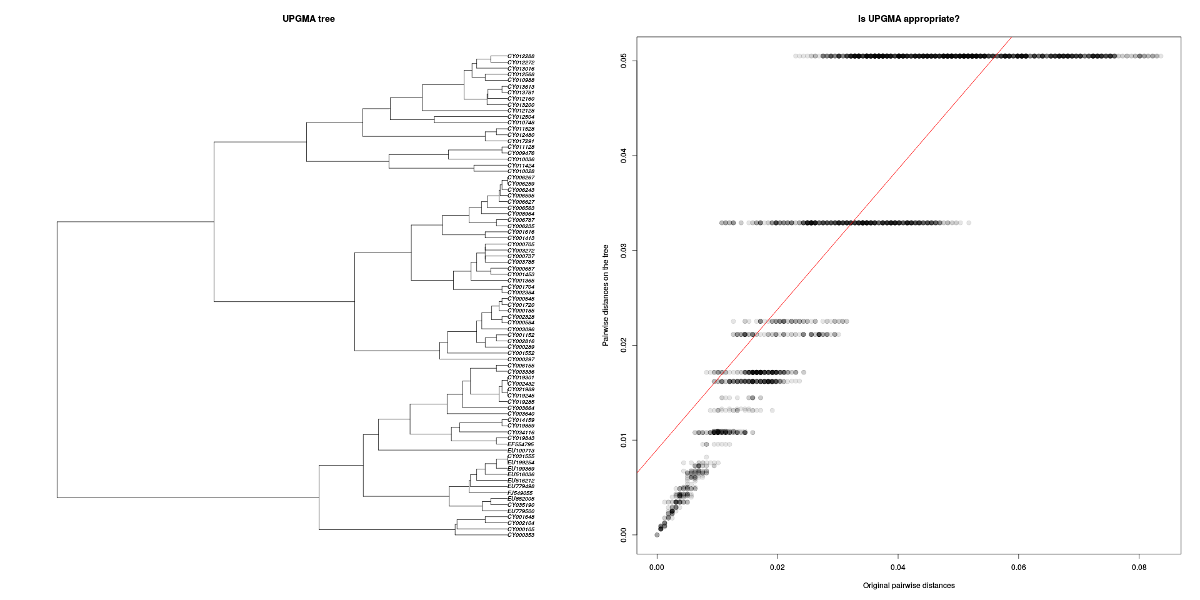
\includegraphics[width=\textwidth]{upgma.png}
  \vfil
  All points in the right graph should be clustered along the red line\ldots
  \vfill
\end{frame}

\subsection{AMOVA} % TODO get percentage of variability

\begin{frame}[fragile]{AMOVA}
  \begin{spluscode}
    # From package pegas (doesn't directly show percentage of variance)
    hauss.pop <- pop(hauss.genind)
    hauss.amova <- pegas::amova(hauss.dist~hauss.pop, data=NULL,
      nperm=1000, is.squared=TRUE)
    hauss.amova
    ...
                    SSD      MSD df
    hauss.pop  30.71923 7.679809  4
    Error     119.58100 2.847167 42
    Total     150.30023 3.267396 46
    ...
  \end{spluscode}
  \begin{itemize}
    \item Analysis of molecular variance tests if there are significant differences among populations (and/or another levels)
%     \item See \texttt{MSD} column for how much of the variance is on which level -- percentage can be calculated as percentage of each level from \texttt{Total}
    \item Another possibility is \texttt{poppr.amova} -- for more complicated hierarchy, see \texttt{?poppr.amova}
  \end{itemize}
\end{frame}

\subsection{MSN}

\begin{frame}[fragile]{Minimum Spanning Network}{Package poppr, based on Bruvo's distance (for SSRs)}
\label{MSN}
\begin{multicols}{2}
  \begin{center}
    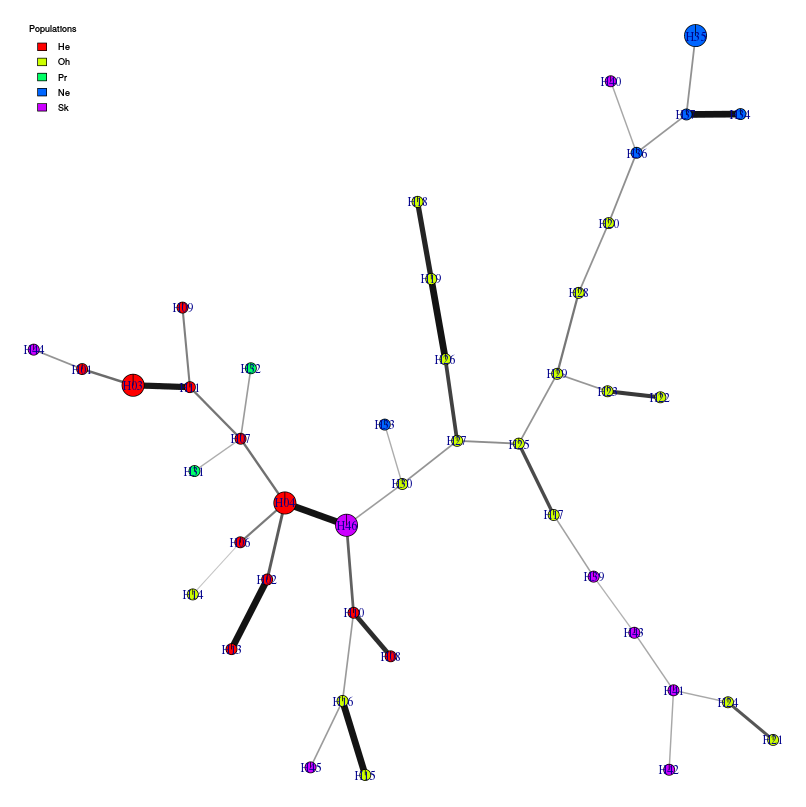
\includegraphics[height=5.5cm]{msn.png}
  \end{center}
  \begin{spluscode}
    ?bruvo.msn # See details...
  \end{spluscode}
  \columnbreak
  \begin{spluscode}
    bruvo.msn(gid=hauss.genind,
      replen=rep(2, 12), loss=TRUE,
      palette=rainbow, vertex.label
      ="inds", gscale=TRUE,
      wscale=TRUE, showplot=TRUE)
    ?msn.poppr # For another data types
    ?imsn # Interactive creation of MSN
  \end{spluscode}
  \begin{center}
    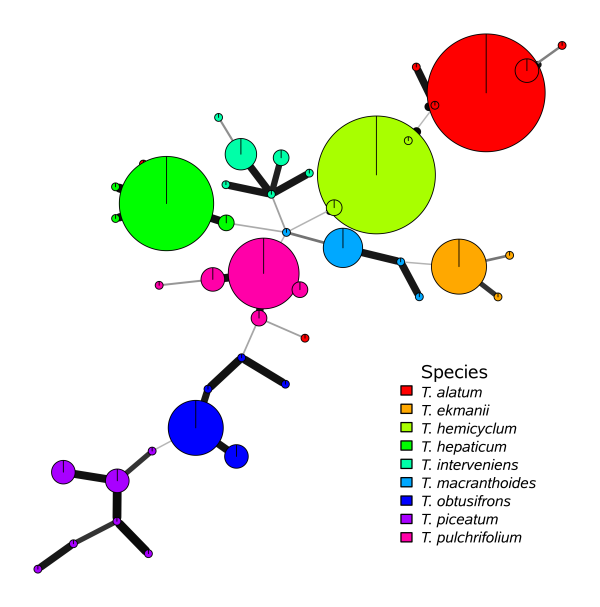
\includegraphics[width=3cm]{msn-bruvo_no_labels.png}
  \end{center}
\end{multicols}
\end{frame}

\subsection{NJ (and UPGMA) tree}

\begin{frame}[fragile]{Calculate and test NJ tree}
  \label{NJ}
  \begin{spluscode}
    # Calculates the tree (try with various distances)
    hauss.nj <- nj(hauss.dist)
    # Test tree quality - plot original vs. reconstructed distance
    plot(as.vector(hauss.dist), as.vector(as.dist(cophenetic(hauss.nj))),
      xlab="Original distance", ylab="Reconstructed distance")
    abline(lm(as.vector(hauss.dist) ~
      as.vector(as.dist(cophenetic(hauss.nj)))), col="red")
    # Linear model for above graph
    summary(lm(as.vector(hauss.dist) ~
      as.vector(as.dist(cophenetic(hauss.nj))))) # Prints summary text
    # Plot a basic tree - see ?plot.phylo for details
    plot.phylo(x=hauss.nj, type="phylogram")
    plot.phylo(x=hauss.nj, type="cladogram", edge.width=2)
    plot.phylo(x=hauss.nj, type="fan", edge.width=2, edge.lty=2)
    plot.phylo(x=hauss.nj, type="radial", edge.color="red",
      edge.width=2, edge.lty=3, cex=2)
    # There are enormous graphical possibilities...
  \end{spluscode}
\end{frame}

\begin{frame}{Choose your tree\ldots}
  \begin{center}
    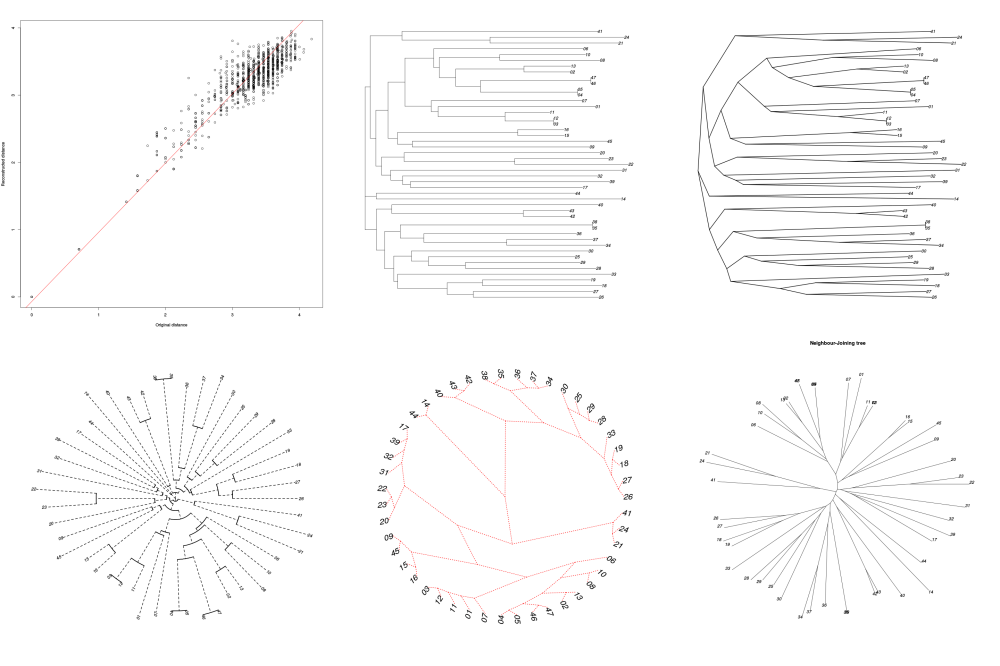
\includegraphics[width=\textwidth-1.5cm]{nj1.png}
  \end{center}
\end{frame}

\begin{frame}[fragile]{Bootstrap}
  \begin{spluscode}
    # boot.phylo() resamples all columns - remove population column first
    hauss.loci.nopop <- hauss.loci
    hauss.loci.nopop[["population"]] <- NULL
    # Calculate the bootstrap
    hauss.boot <- boot.phylo(phy=hauss.nj, x=hauss.loci.nopop,
      FUN=function(XXX) nj(dist(loci2genind(XXX))), B=1000)
    # boot.phylo returns NUMBER of replicates - NO PERCENTAGE
    # Plot the tree
    plot.phylo(x=hauss.nj, type="unrooted", main="Neighbour-Joining tree")
    # Labels for nodes - bootstrap - see ?nodelabels for graphical settings
    nodelabels(text=round(hauss.boot/10))
    ?boot.phylo # See details
    # Another possibility
    hauss.aboot <- aboot(x=hauss.genind, tree="nj", distance=nei.dist,
      sample=100) # Bootstrap values are in slot node.label
    # Plot the tree, explicitly display node labels
    plot.phylo(x=hauss.aboot, show.node.label=TRUE)
    ?aboot # Package poppr
  \end{spluscode}
\end{frame}

\begin{frame}[fragile]{Nicer trees}
  \begin{footnotesize}
  \begin{spluscode}
    ## Plot a nice tree with colored tips
    plot.phylo(x=hauss.nj, type="unrooted", show.tip=F, lwd=3, main="NJ")
    # Labels for nodes - bootstrap - see ?nodelabels for graphical settings
    nodelabels(text=round(hauss.boot/10))
    # Colored labels - creates vector of colors according to populations
    nj.rainbow<-colorRampPalette(rainbow(length(levels(pop(hauss.genind)))))
    tiplabels(text=hauss.genind$ind.names, bg=fac2col(x=hauss.genind$pop,
      col.pal=nj.rainbow)) # Colored tips
    ## Plot BW tree with tip symbols and legend
    plot.phylo(x=hauss.nj, type="cladogram", show.tip=F, lwd=3, main="NJ")
    axisPhylo() # Add axis with distances
    # From node labels let's remove unneeded frame
    nodelabels(text=round(hauss.boot/10), frame="none", bg="white")
    # As tip label we use only symbols - see ?points for graphical details
    tiplabels(frame="none", pch=rep(0:4,times=c(13,17,2,6,9)), lwd=2, cex=2)
    # Plot a legend explaining symbols
    legend(x="topleft", legend=c("He", "Oh", "Pr", "Ne", "Sk"), 
      border="black", pch=0:4, pt.lwd=2, pt.cex=2, bty="o", bg="lightgrey",
      box.lwd=2, cex=1.2, title="Populations")
  \end{spluscode}
  \end{footnotesize}
\end{frame}

\begin{frame}{Choose your tree\ldots}
  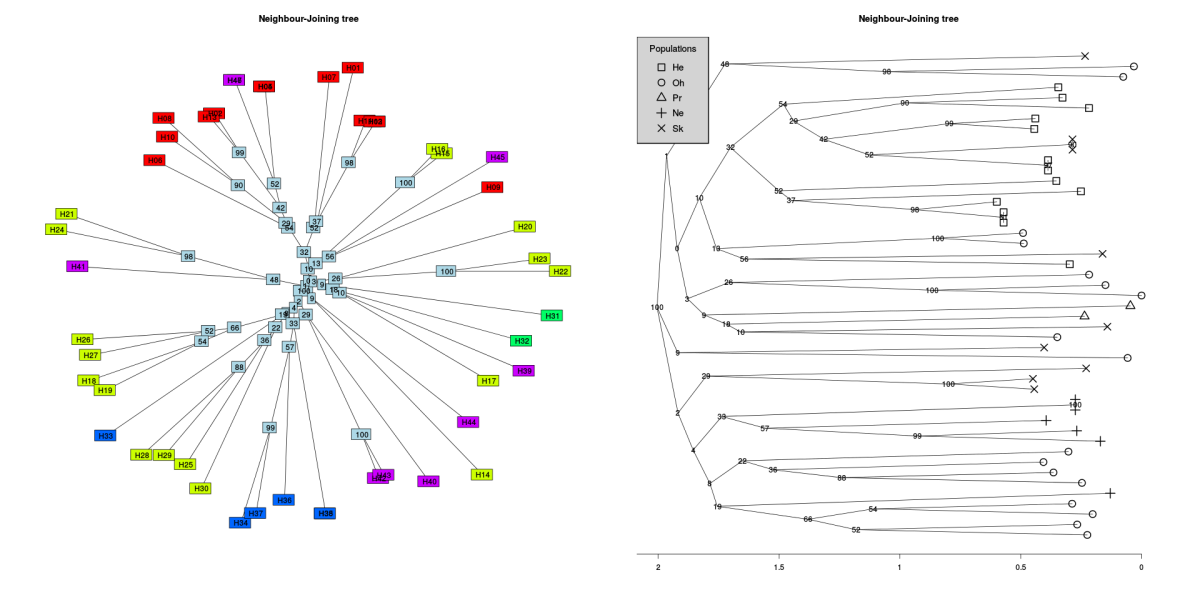
\includegraphics[width=\textwidth]{nj2.png}
\end{frame}

\begin{frame}[fragile]{Trees based on Bruvo's distance}{Package poppr (bootstrap is incorporated within the function)}
  \begin{spluscode}
    # There are currently problems with compatibility with newest ape...
    # NJ
    hauss.nj.bruvo <- bruvo.boot(gid=hauss.genind, replen=rep(2, 12),
      sample=1000, tree="nj", showtree=TRUE, cutoff=1, quiet=FALSE)
    plot.phylo(x=hauss.nj.bruvo, type="unrooted", show.tip=FALSE,
      lwd=3, main="Neighbor-Joining tree.")
    # Call node labels as phylo$node.labels or phylo[["node.labels"]]
    nodelabels(hauss.nj.bruvo[["node.labels"]]) 
    tiplabels(hauss.nj.bruvo[["tip.label"]], bg=fac2col(x=hauss.genind$pop,
      col.pal=nj.rainbow))
    # UPGMA
    hauss.upgma <- bruvo.boot(gid=hauss.genind, replen=rep(2, 12),
      sample=1000, tree="upgma", showtree=TRUE, cutoff=1, quiet=FALSE)
    plot.phylo(hauss.upgma, type="unrooted", show.tip=FALSE, lwd=3,
      main="UPGMA tree")
    nodelabels(hauss.upgma[["node.labels"]])
    tiplabels(hauss.upgma[["tip.label"]], bg=fac2col(x=hauss.genind@pop,
      col.pal=nj.rainbow))
  \end{spluscode}
\end{frame}

\begin{frame}{Choose your tree\ldots}
  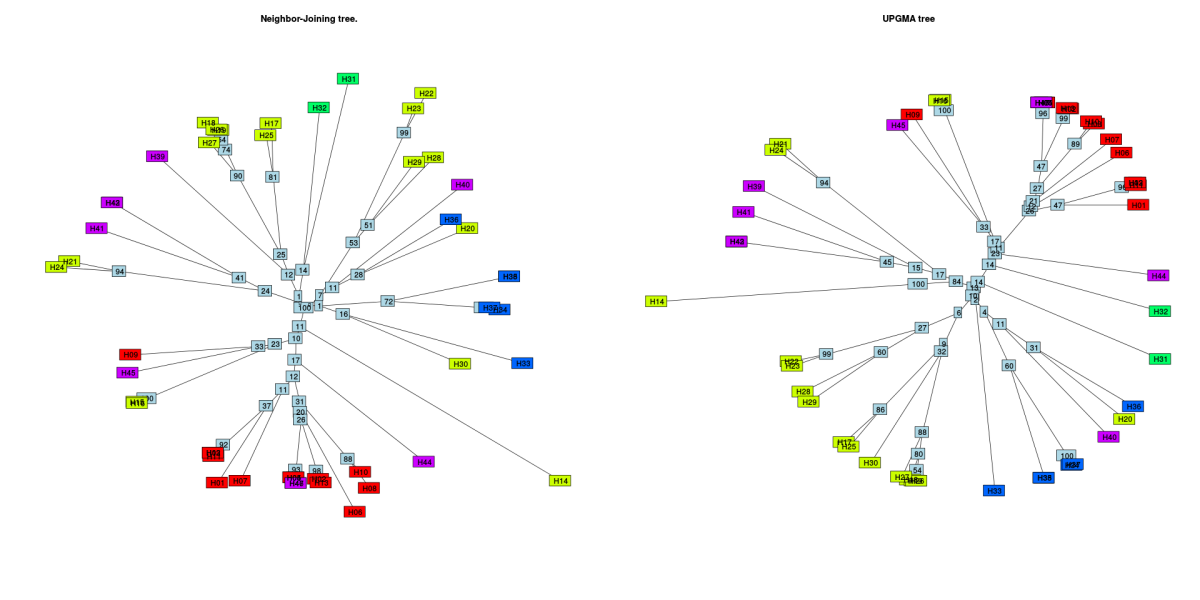
\includegraphics[width=\textwidth]{nj-upgma-bruvo.png}
\end{frame}

% \begin{frame}[fragile]{NJ tree of populations} % FIXME rewrite the function for new version of APE
%   \begin{spluscode}
%     # NJ tree of populations
%     hauss.nj.pop <- nj(hauss.dist.pop)
%     # Bootstrap - source() loads external scripts
%     # boot.phylo doesn't work for population trees
%     source("https://soubory.trapa.cz/rcourse/boot_phylo_nj_pop.r")
%     hauss.boot.pop <- boot.phylo.nj.pop(hauss.nj.pop, hauss.genind, 1000)
%     # Plot a tree
%     plot(hauss.nj.pop, type="radial", cex=1.2, lwd=3,
%       main="Neighbor-Joining tree of populations")
%     # Labels - bootstrap
%     nodelabels(round(hauss.boot.pop/10), frame="none")
%     # Print information about phylo object
%     print.phylo(hauss.nj.pop)
%   \end{spluscode}
% \end{frame}

\begin{frame}[fragile]{NJ tree based on DNA sequences}
  \begin{spluscode}
    # Calculate the tree
    usflu.tree <- nj(X=usflu.dist)
    # Plot it
    plot.phylo(x=usflu.tree, type="unrooted", show.tip=FALSE)
    title("Unrooted NJ tree")
    # Coloured tips
    usflu.pal <- colorRampPalette(topo.colors(length(levels(as.factor(
      usflu.annot[["year"])))))
    # Tip labels
    tiplabels(text=usflu.annot$year, bg=num2col(usflu.annot$year,
      col.pal=usflu.pal), cex=0.75)
    # Legend - describing years - pretty() automatically shows best
    # values from given range, num2col() selects colors from color scale
    legend(x="bottomright", fill=num2col(x=pretty(x=1993:2008, n=8),
      col.pal=usflu.pal), leg=pretty(x=1993:2008, n=8), ncol=1)
  \end{spluscode}
\end{frame}

\begin{frame}[fragile]{Root the tree}
  \begin{spluscode}
    # Root the tree - "outgroup" is name of accession (in quotation
    # marks) or number (position within phy object)
    usflu.tree.rooted <- root(phy=usflu.tree, outgroup=1)
    # Plot it
    plot.phylo(x=usflu.tree.rooted, show.tip=FALSE, edge.width=2)
    title("Rooted NJ tree")
    # Labeling of tips
    tiplabels(text=usflu.annot$year, bg=transp(num2col(x=usflu.annot$year,
      col.pal=usflu.pal), alpha=0.7), cex=0.75, fg="transparent")
    # Add axis with phylogenetic distance
    axisPhylo()
    # Legend - describing years - pretty() automatically shows best
    # values from given range, num2col() selects colors from color scale
    legend(x="topright", fill=num2col(x=pretty(x=1993:2008, n=8),
      col.pal=usflu.pal), leg=pretty(x=1993:2008, n=8), ncol=1)
  \end{spluscode}
\end{frame}

\begin{frame}[fragile]{Bootstrap rooted tree}
  \begin{spluscode}
    # Calculate it
    usflu.boot <- boot.phylo(phy=usflu.tree.rooted, x=usflu.dna,
      FUN=function(EEE) root(nj(dist.dna(EEE, model="TN93")),
      outgroup=1), B=1000)
    # Plot the tree
    plot.phylo(x=usflu.tree.rooted, show.tip=FALSE, edge.width=2)
    title("NJ tree + bootstrap values")
    tiplabels(frame="none", pch=20,
      col=transp(num2col(x=usflu.annot[["year"]], col.pal=usflu.pal),
      alpha=0.7), cex=3.5, fg="transparent")
    axisPhylo()
    # Legend - describing years - pretty() automatically shows best
    # values from given range, num2col() selects colors from color scale
    legend(x="topright", fill=num2col(x=pretty(x=1993:2008, n=8),
      col.pal=usflu.pal), leg=pretty(x=1993:2008, n=8), ncol=1)
    # Plots bootstrap support - note usflu.boot contains raw numbers
    # transform it into percent
    nodelabels(text=round(usflu.boot/10), cex=0.75)
  \end{spluscode}
\end{frame}

\begin{frame}[fragile]{Collapse branches with low bootstrap support}
  \begin{spluscode}
    usflu.tree.temp <- usflu.tree.rooted
    # Determine branches with low support - note BS values are in raw
    # numbers - use desired percentage with respect to number of bootstraps
    usflu.tocollapse <- match(x=which(usflu.boot < 700)+
      length(usflu.tree.rooted$tip.label), table=usflu.tree.temp$edge[,2])
    # Set length of bad branches to zero
    usflu.tree.temp$edge.length[usflu.tocollapse] <- 0
    # Create new tree
    usflu.tree.collapsed <- di2multi(phy=usflu.tree.temp, tol=0.00001)
    # Plot the consensus tree
    plot.phylo(x=usflu.tree.collapsed, show.tip=FALSE, edge.width=2)
    title("NJ tree after collapsing weak nodes")
    tiplabels(text=usflu.annot$year,
      bg=transp(num2col(x=usflu.annot[["year"]], col.pal=usflu.pal),
      alpha=0.7), cex=0.5, fg="transparent")
    axisPhylo()
    legend(x="topright", fill=num2col(x=pretty(x=1993:2008, n=8),
      col.pal=usflu.pal), leg=pretty(x=1993:2008, n=8), ncol=1)
  \end{spluscode}
\end{frame}

\begin{frame}{The trees}
  \begin{center}
    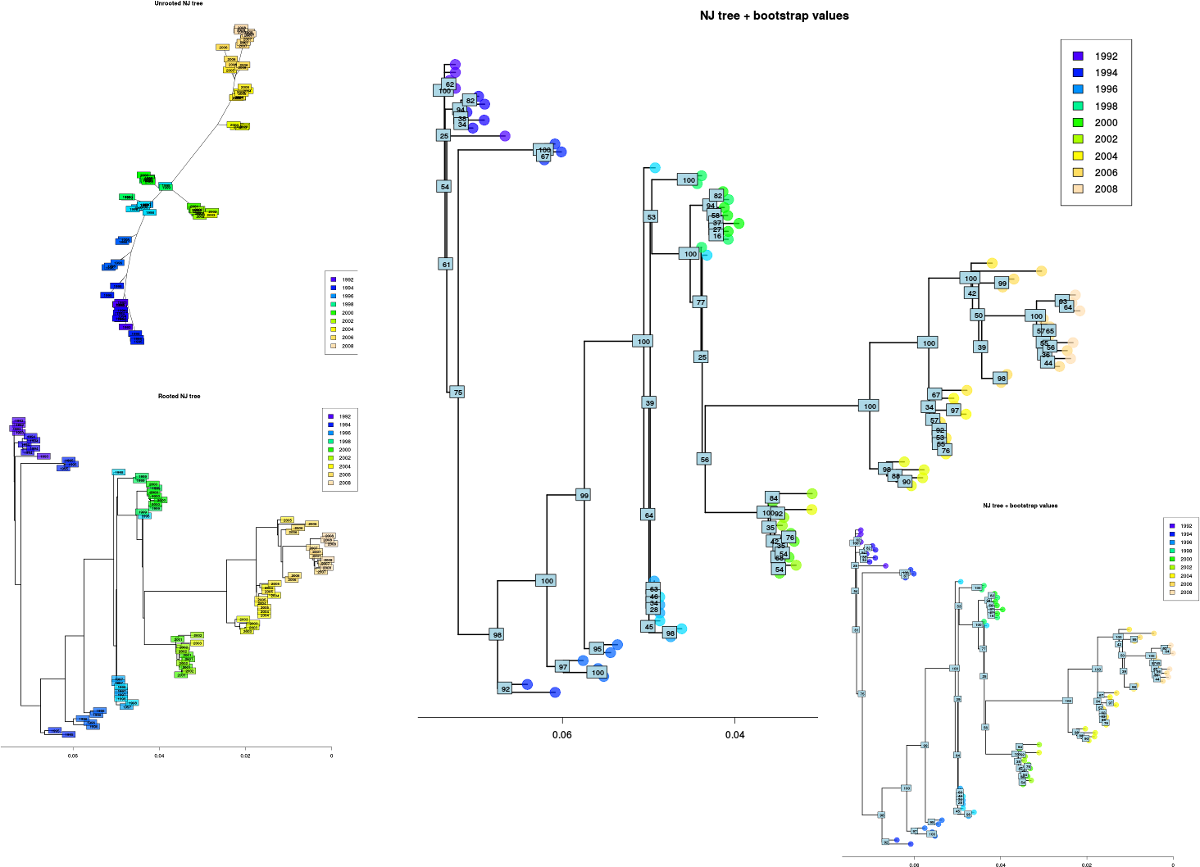
\includegraphics[width=\textwidth-2.5cm]{nj_dna.png}
  \end{center}
\end{frame}

\begin{frame}{NJ is death. Long live NJ!}
  \label{NJ-replacement}
  \begin{itemize}
  \item ``Basic'' NJ has many limitations (problems with missing data, chaining of individuals,~\ldots) -- there are several tries to overcome them
  \item Package \texttt{phangorn} has functions \texttt{NJ()} and unweighted version \texttt{UNJ()}
  \item Package \texttt{ape} has functions \texttt{njs()} and \texttt{bionjs()} which are designed to perform well on distances with (more) missing values
  \item Function \texttt{bionj()} from \texttt{ape} implements BIONJ algorithm
  \item FastME functions (package \texttt{ape}) perform the minimum evolution algorithm and aim to be replacement of NJ -- read \texttt{?fastme} before use
  \item All those functions read distance matrix and their usage is same as with ``classical'' \texttt{nj()} (read manual pages before using them) -- it is also from package \texttt{ape}
  \end{itemize}
\end{frame}

\subsection{PCoA}

\begin{frame}[fragile]{PCoA I}
  \label{pcoa}
  \begin{spluscode}
    hauss.pcoa <- dudi.pco(d=dist(x=scaleGen(x=hauss.genind, center=TRUE,
      scale=FALSE, truenames=TRUE), method="euclidean"), scannf=FALSE,
      nf=3)
    # Basic display
    s.label(dfxy=hauss.pcoa$li, clabel=0.75)
    # To plot different axes use for example dfxy=hauss.pcoa$li[c(2, 3)]
    # Add kernel density
    s.kde2d(dfxy=hauss.pcoa$li, cpoint=0, add.plot=TRUE)
    # Adds histogram of Eigenvalues
    add.scatter.eig(w=hauss.pcoa$eig, nf=3, xax=1, yax=2,
      posi="bottomleft", sub="Eigenvalues")
    # Colored display according to populations
    # Creates vector of colors according to populations
    hauss.pcoa.col <- rainbow(length(levels(pop(hauss.genind))))
    s.class(dfxy=hauss.pcoa$li, fac=pop(hauss.genind), col=hauss.pcoa.col)
    add.scatter.eig(w=hauss.pcoa$eig, nf=3, xax=1, yax=2,
      posi="bottomleft", sub="Eigenvalues")
    title("Principal Coordinates Analysis") # Adds title to the graph
  \end{spluscode}
\end{frame}

\begin{frame}[fragile]{PCoA II}
\begin{multicols}{2}
  \begin{center}
    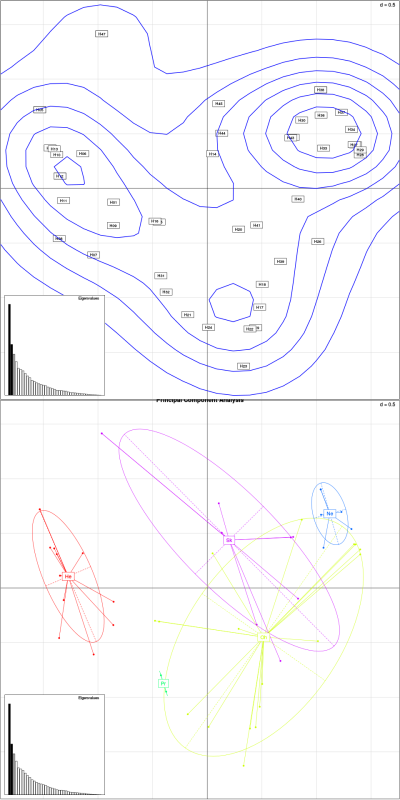
\includegraphics[height=6.5cm]{pcoa.png}
  \end{center}
  \columnbreak
  \begin{spluscode}
    hauss.pcoa.bruvo <- dudi.pco(d=	
      bruvo.dist(pop=hauss.genind,
      replen=rep(2, 12)), scannf=F,
      nf=3)
    s.class(dfxy=hauss.pcoa.bruvo$li,
      fac=pop(hauss.genind),
      col=hauss.pcoa.col)
    add.scatter.eig(hauss.pcoa.bruvo$
      eig, posi="bottomright", 3,1,2)
    # Another possibility for colored
    # plot (see ?colorplot for details)
    colorplot(xy=hauss.pcoa$li[c(1,2)],
      X=hauss.pcoa$li, transp=TRUE,
      cex=3, xlab="PC 1", ylab="PC 2")
    title(main="PCoA, axes 1 and 3")
    abline(v=0, h=0, col="grey", lty=2)
  \end{spluscode}
\end{multicols}
\end{frame}

\begin{frame}{PCoA -- Bruvo and colorplot}
  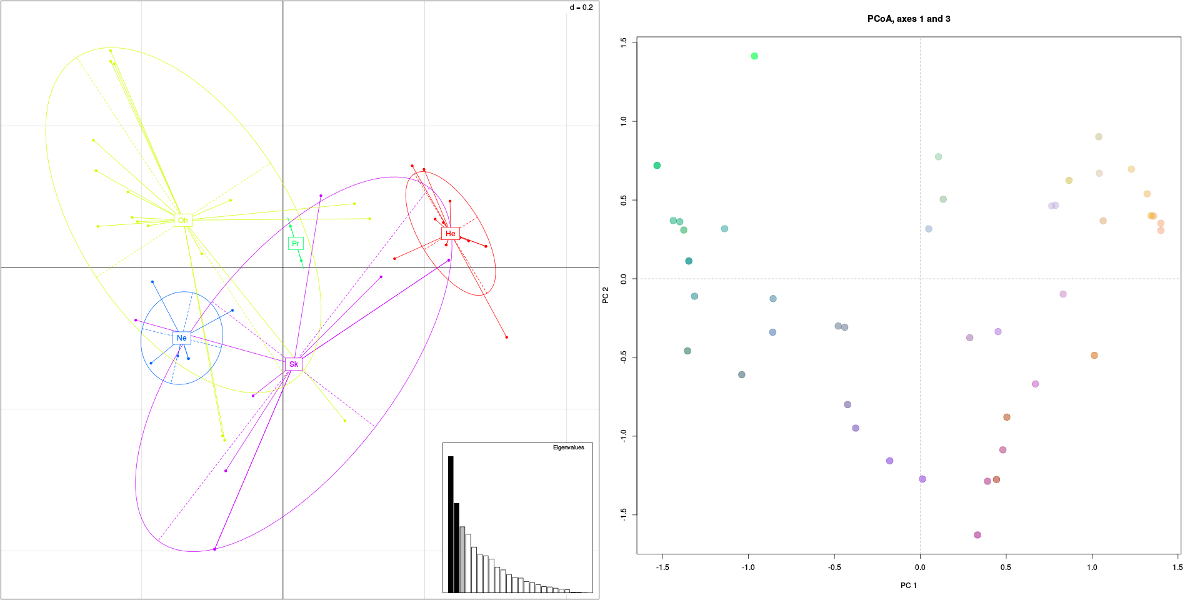
\includegraphics[width=\textwidth]{pcoa-dalsi.png}
\end{frame}

\section{DAPC}

\begin{frame}[fragile]{DAPC}
  \label{DAPC}
  \begin{itemize}
    \item Discriminant Analysis of Principal components (\href{http://bmcgenet.biomedcentral.com/articles/10.1186/1471-2156-11-94}{Jombart et al. 2010})
    \item Runs K-means Bayesian clustering on data transformed with PCA (reduces number of variables, speeds up process)
    \item Finally it runs discriminant analysis (DA) to maximize differences among groups
    \item Various modes of displaying of results -- ``Structure-like'', ``PCA-like'' and more
    \item More information at \url{http://adegenet.r-forge.r-project.org/} and \texttt{adegenetTutorial("dapc")}
    \item If following commands would seem too complicated to you, try web interface by this command:
  \end{itemize}
  \begin{spluscode}
    adegenetServer("DAPC") # Recommended to open in Google Chrome/Chromium
  \end{spluscode}
\end{frame}

\begin{frame}{Principal difference between PCA and DA}
  \begin{center}
    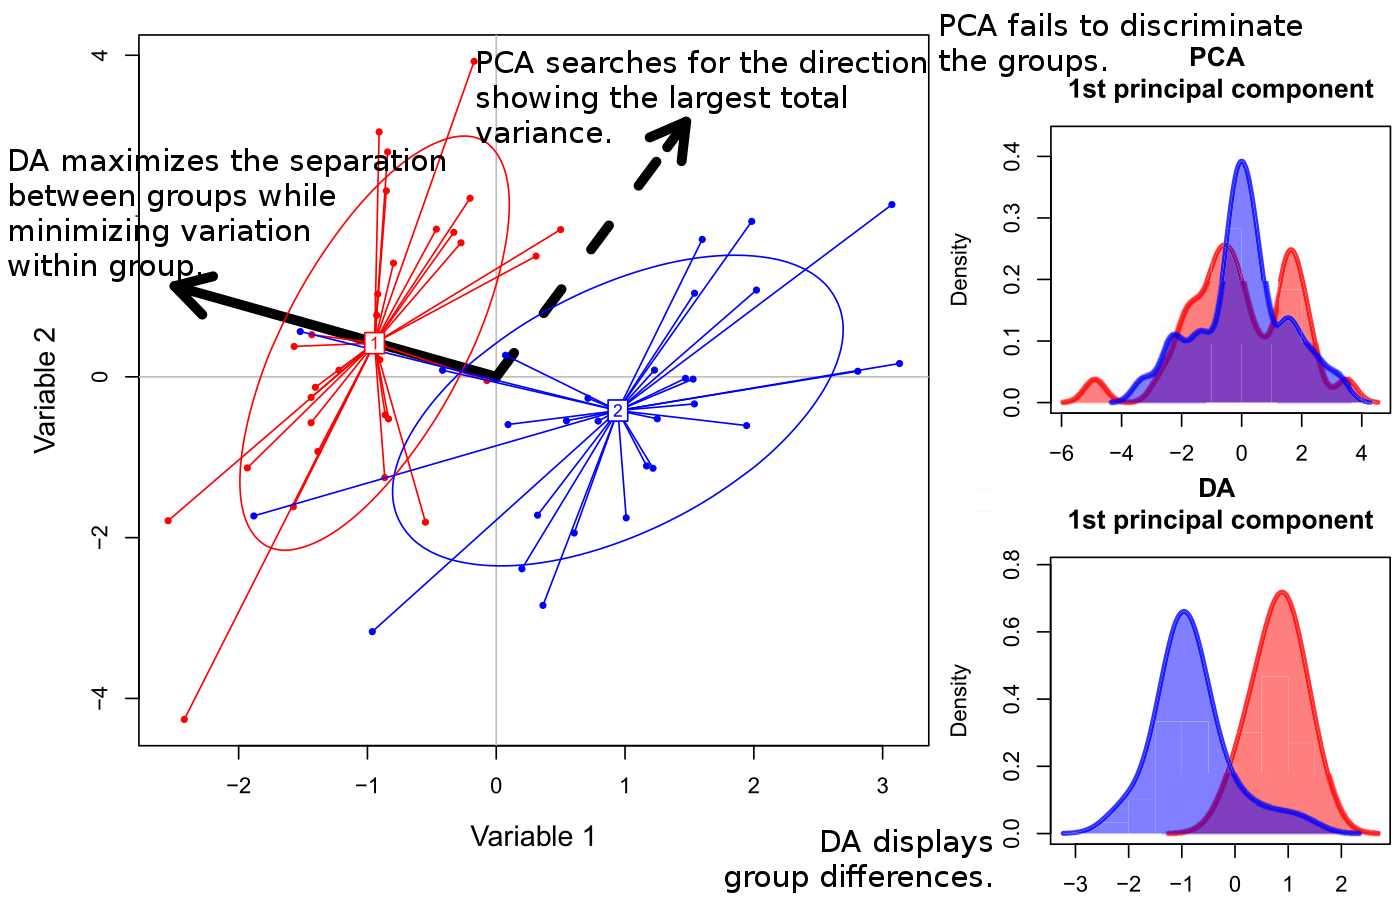
\includegraphics[height=6cm]{dapc-da-pca.png}
  \end{center}
\end{frame}

\subsection{Bayesian clustering}

\begin{frame}[fragile]{K-find -- Bayesian K-means clustering}
  \begin{spluscode}
    # Retain all informative PC (here about 35)
    # According to second graph select best K (here 2 or 3)
    # Now we select K=2 and later rerun the analysis for K=3 (lines 14-18)
    hauss.kfind <- find.clusters(x=hauss.genind, stat="BIC",
      choose.n.clust=TRUE, max.n.clust=10, n.iter=100000, n.start=100,
      scale=FALSE, truenames=TRUE)
    # See results as text
    table(pop(hauss.genind), hauss.kfind$grp)
    hauss.kfind
    # Graph showing table of original and inferred populations and
    # assignment of individuals
    table.value(df=table(pop(hauss.genind), hauss.kfind$grp), col.lab=
      paste("Inferred\ncluster", 1:length(hauss.kfind$size)), grid=TRUE)
    # For K=3 - note parameters n.pca and n.clust - we just rerun the
    # analysis and when results are stable, no problem here
    hauss.kfind3 <- find.clusters(x=hauss.genind, n.pca=35, n.clust=3,
      stat="BIC", choose.n.clust=FALSE, max.n.clust=10, n.iter=100000,
      n.start=100, scale=FALSE, truenames=TRUE)
  \end{spluscode}
\end{frame}

\begin{frame}[fragile]{K-find outputs}
\begin{multicols}{2}
  \begin{itemize}
    \item Cumulative variance of axis
    \item BIC helps to select the best K
    \item Original and inferred groups
  \end{itemize}
  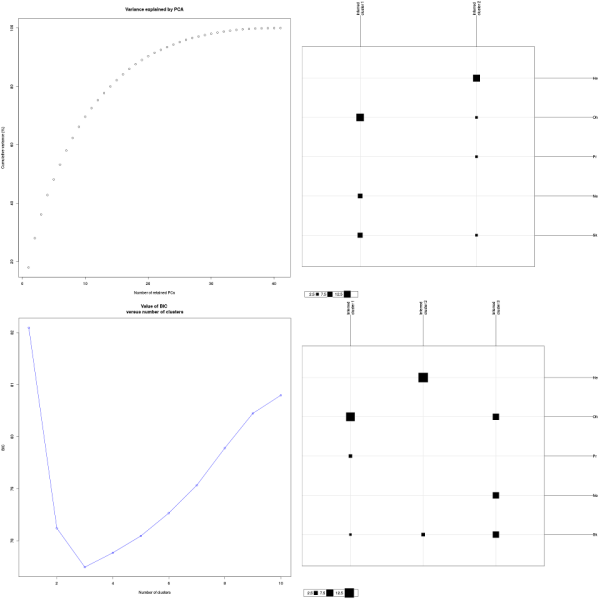
\includegraphics[height=5cm]{kmeans.png}
  \begin{spluscode}
    # See results as text
    table(pop(hauss.genind),
      hauss.kfind3$grp)
    hauss.kfind3
    # Graph showing table of original
    # and inferred populations and
    # assignment of individuals
    table.value(
      df=table(pop(hauss.
      genind), hauss.kfind3$grp),
      col.lab=paste("Inferred\n
      cluster",
      1:length(hauss.kfind3$size)),
      grid=TRUE)
    # If needed, use custom text for
    # parameter col.lab=c("...", "...")
    # as many labels as inferred groups
  \end{spluscode}
\end{multicols}
\end{frame}

\subsection{Discriminant analysis and visualization}

\begin{frame}[fragile]{DAPC code I}
  \begin{spluscode}
    ## K=2
    # Create DAPC
    # Number of informative PC (Here 15, adegenet recommends < N/3). Select
    # number of informative DA (here only one is available - no PCA graph)
    hauss.dapc <- dapc(x=hauss.genind, pop=hauss.kfind$grp, center=TRUE,
      scale=FALSE, var.contrib=TRUE, pca.info=TRUE, truenames=TRUE)
    # Information
    hauss.dapc
    # Density function - only for first axis here!
    scatter(x=hauss.dapc, xax=1, yax=1, main="DAPC", bg="white", solid=0.5,
      leg=TRUE, txt.leg=c("Group 1", "Group 2"), posi.leg="topright")
    # Assignment of individuals to clusters
    assignplot(x=hauss.dapc)
    # Structure-like plot
    compoplot(x=hauss.dapc, xlab="Individuals", leg=FALSE)
    # Loadingplot - alleles the most adding to separation of individuals
    loadingplot(x=hauss.dapc$var.contr)
  \end{spluscode}
\end{frame}

\begin{frame}{DAPC for K=2}
  \begin{center}
    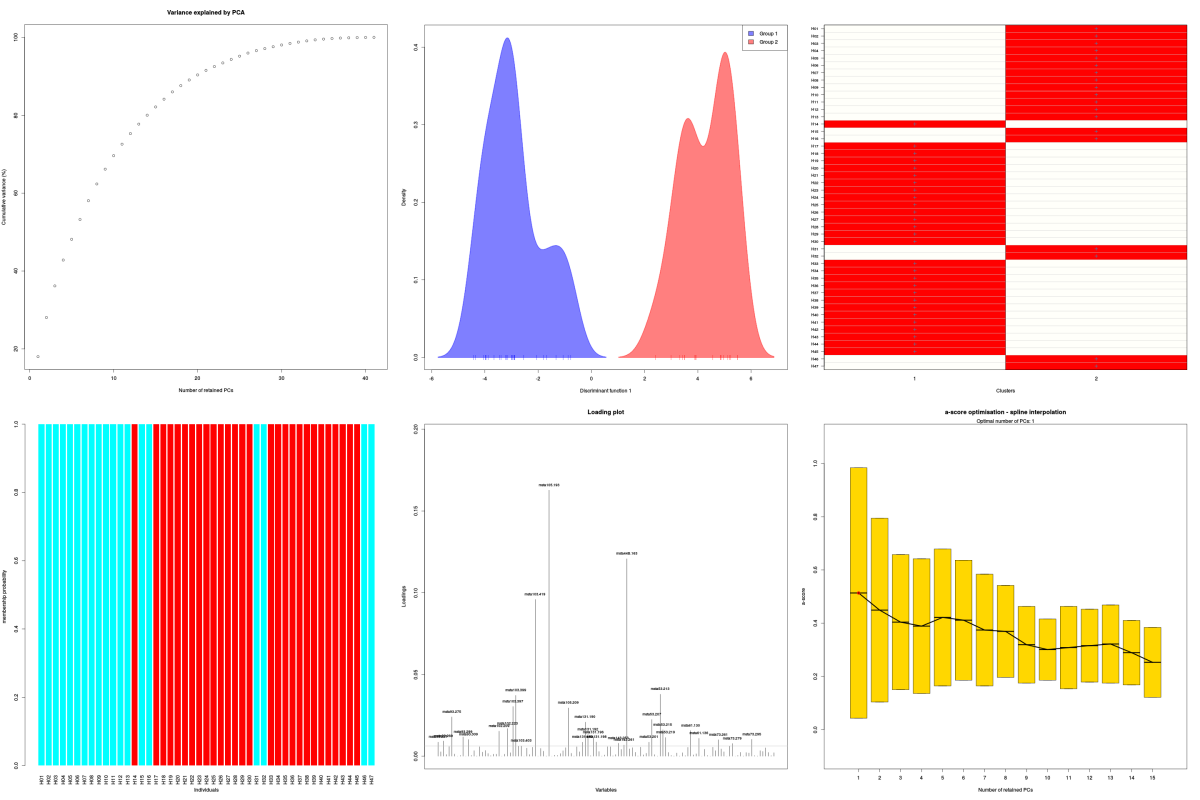
\includegraphics[width=\textwidth-1.5cm]{dapc2.png}
  \end{center}
\end{frame}

\begin{frame}[fragile]{DAPC code II}
  \begin{spluscode}
    # alfa-score - according to number of PC axis
    optim.a.score(x=hauss.dapc)
    ## K=3
    # Create DAPC
    # Number of informative PC (Here 15, adegenet recommends < N/3)
    # Select number of informative DA (here 2 - usually keep all of them)
    hauss.dapc3 <- dapc(x=hauss.genind, pop=hauss.kfind3$grp, center=TRUE,
      scale=FALSE, var.contrib=TRUE, pca.info=TRUE, truenames=TRUE)
    # Information
    hauss.dapc
    # A la PCA graph
    scatter(x=hauss.dapc3, main="DAPC, Taraxacum haussknechtii",
      bg="white", cex=3, clab=0, col=rainbow(3), posi.da="bottomleft",
      scree.pca=TRUE, posi.pca="bottomright", leg=TRUE,
      txt.leg=c("Group 1", "Group 2", "Group 3"), posi.leg="topleft")
  \end{spluscode}
  \begin{itemize}
    \item Especially graphical parameters have huge possibilities\ldots
    \item See \texttt{?scatter} and play with it\ldots
  \end{itemize}
\end{frame}

\begin{frame}{DAPC for K=3}
  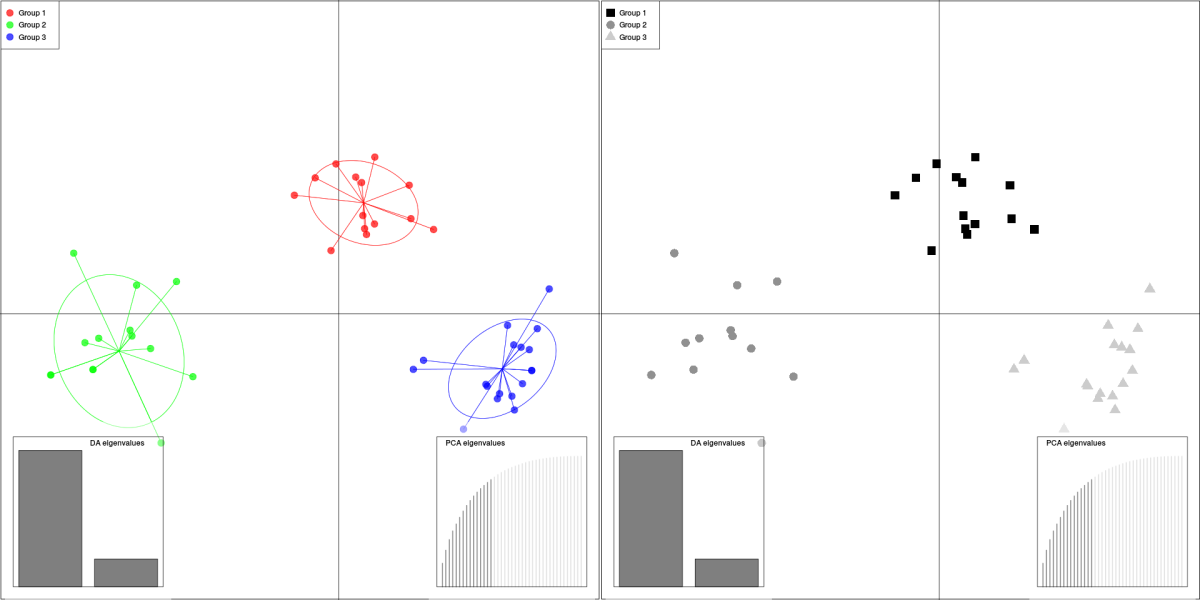
\includegraphics[width=\textwidth]{dapc3.png}
\end{frame}

\begin{frame}[fragile]{DAPC code III}
  \begin{spluscode}
    # Same in BW
    scatter(x=hauss.dapc3, main="DAPC, Taraxacum haussknechtii",
      bg="white", pch=c(15:17), cell=0, cstar=0, solid=1, cex=2.5, clab=0,
      col=grey.colors(3, start=0, end=0.8, gamma=2, alpha=0), posi.da=
      "bottomleft", scree.pca=TRUE, posi.pca="bottomright", leg=TRUE,
      txt.leg=c("Group 1", "Group 2", "Group 3"), posi.leg="topleft")
    # Density function - only for first axis here!
    scatter(x=hauss.dapc3, xax=1, yax=1, main="DAPC", bg="white", solid=0.5,
      leg=T, txt.leg=c("Group 1", "Group 2", "Group 3"), posi.leg="topleft")
    # Assignment of individuals to clusters
    assignplot(hauss.dapc3)
    # Structure-like plot
    compoplot(hauss.dapc3, xlab="Individuals", leg=FALSE)
    # Loadingplot - alleles the most adding to separation of individuals
    loadingplot(hauss.dapc3$var.contr)
    # alfa-score - according to number of PC axis
    optim.a.score(hauss.dapc3)
  \end{spluscode}
\end{frame}

\begin{frame}{DAPC for K=3, extra information}
  \begin{center}
    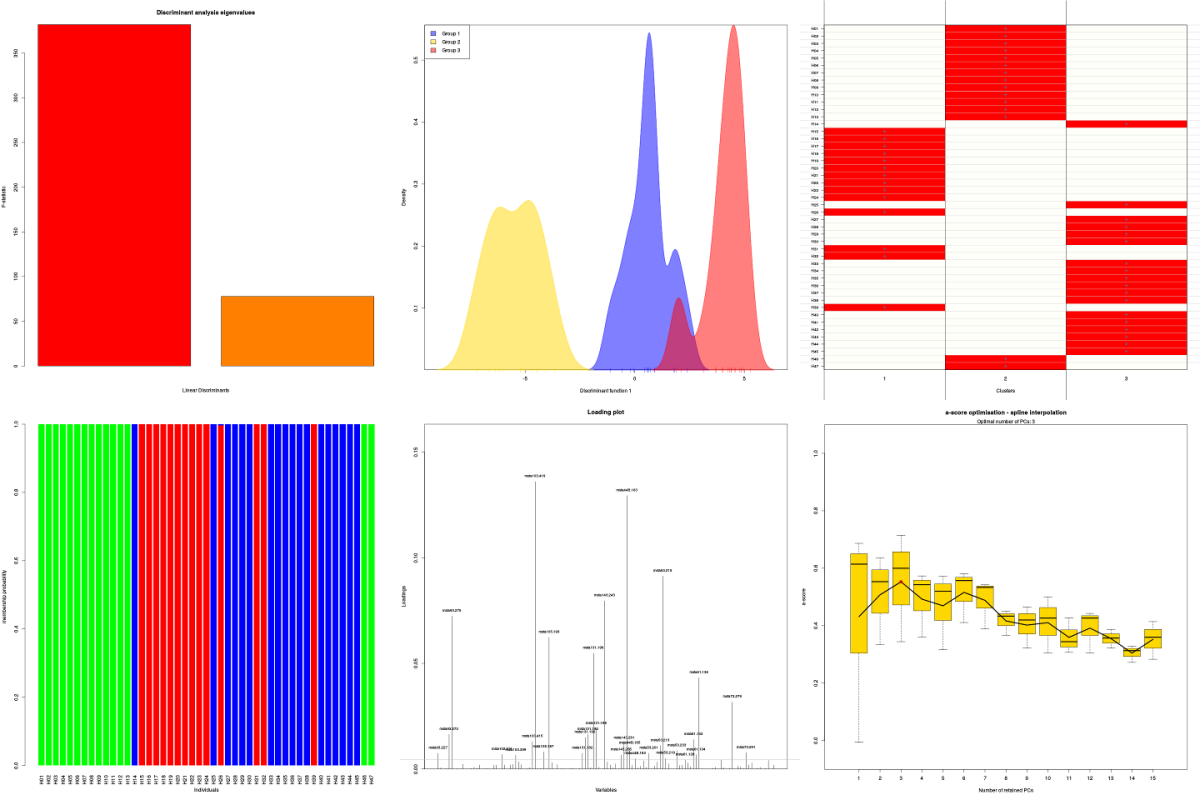
\includegraphics[width=\textwidth-1.5cm]{dapc3-extra.png}
  \end{center}
\end{frame}

\begin{frame}{Another DAPC example}
  \begin{center}
    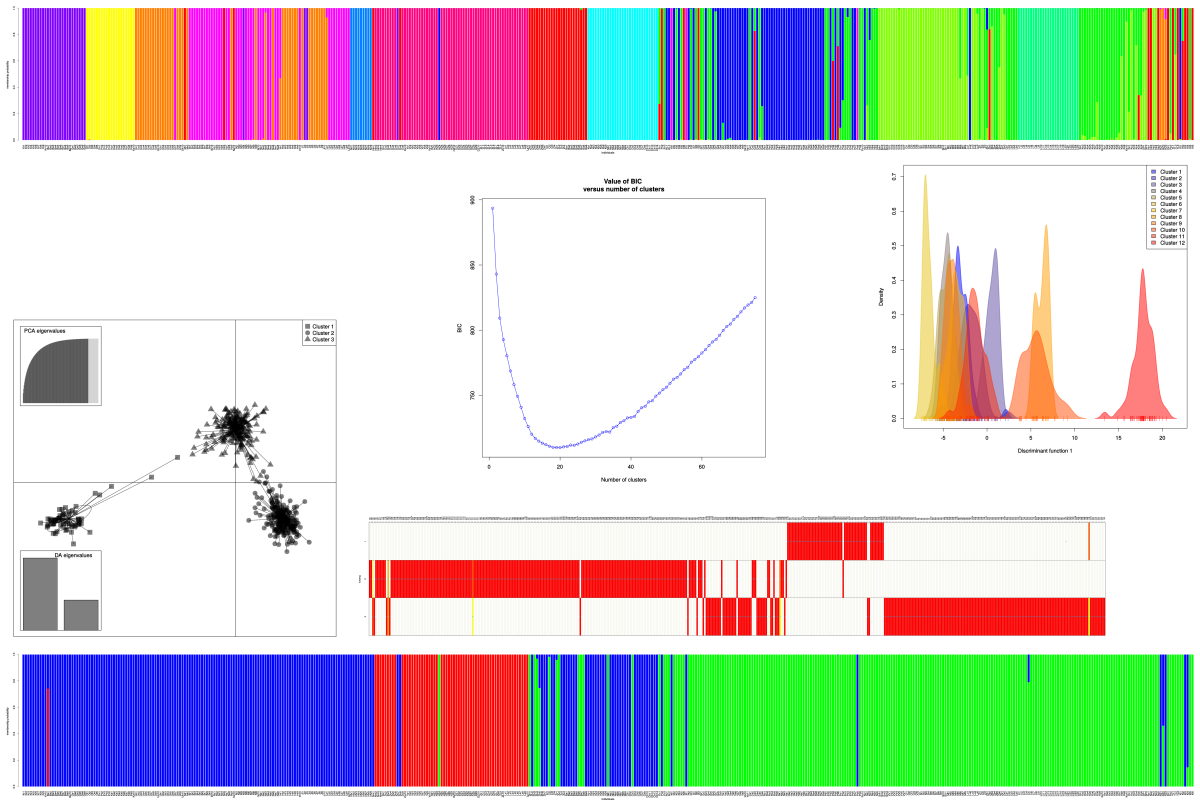
\includegraphics[width=\textwidth-1.5cm]{dapc.png}
  \end{center}
\end{frame}

\section{SNP}

\begin{frame}[fragile]{Special functions to work with huge SNP data sets}
  \begin{spluscode}
    # Plot of missing data (white) and number of 2nd alleles
    glPlot(x=usflu.genlight, legend=TRUE, posi="topleft")
    # Sum of the number of second allele in each SNP
    usflu.freq <- glSum(usflu.genlight)
    # Plot distribution of (second) allele frequencies
    hist(x=usflu.freq, proba=TRUE, col="gold", xlab="Allele
      frequencies", main="Distribution of (second) allele frequencies")
    lines(x=density(usflu.freq)$x, y=density(usflu.freq)$y*1.5,
      col="red", lwd=3 )
    # Mean number of second allele in each SNP
    usflu.mean <- glMean(usflu.genlight)
    usflu.mean <- c(usflu.mean, 1-usflu.mean)
    # Plot distribution of allele frequencies
    hist(x=usflu.mean, proba=TRUE, col="darkseagreen3",
      xlab="Allele frequencies", main="Distribution of allele
      frequencies", nclass=20)
    lines(x=density(usflu.mean, bw=0.05)$x, y=density(usflu.mean,
      bw=0.05)$y*2, lwd=3)
  \end{spluscode}
\end{frame}

\begin{frame}[fragile]{Number of missing values in each locus}
  \begin{spluscode}
    # Play with bw parameter to get optimal image
    usflu.na.density <- density(glNA(usflu.genlight), bw=10)
    # Set range of xlim parameter from 0 to the length
    # of original alignment
    plot(x=usflu.na.density, type="n", xlab="Position in the alignment",
      main="Location of the missing values (NA)", xlim=c(0, 1701))
    polygon(c(usflu.na.density$x, rev(usflu.na.density$x)),
      c(usflu.na.density$y, rep(0, length(usflu.na.density$x))),
      col=transp("blue", alpha=0.3))
    points(glNA(usflu.genlight), rep(0, nLoc(usflu.genlight)), 
      pch="|", cex=2, col="blue")
  \end{spluscode}
  \begin{itemize}
    \item Those tools are designed mainly for situation when having multiple (nearly) complete genomes -- not needed for smaller (normal) datasets
    \item Lets keep hoping in fast development of computers\ldots
    \item \alert{Note for Windows users:} To speed up the processing, \texttt{gl*} functions use parallelisation library, which is not available on Windows -- add parameter \texttt{parallel=FALSE} to be able to use them on Windows
  \end{itemize}
\end{frame}

\begin{frame}{Basic information about SNP: distribution of 2$^{nd}$ allele frequencies, missing data and number of 2$^{nd}$ allele, distribution of allele frequencies, and number of missing values in each locus}
  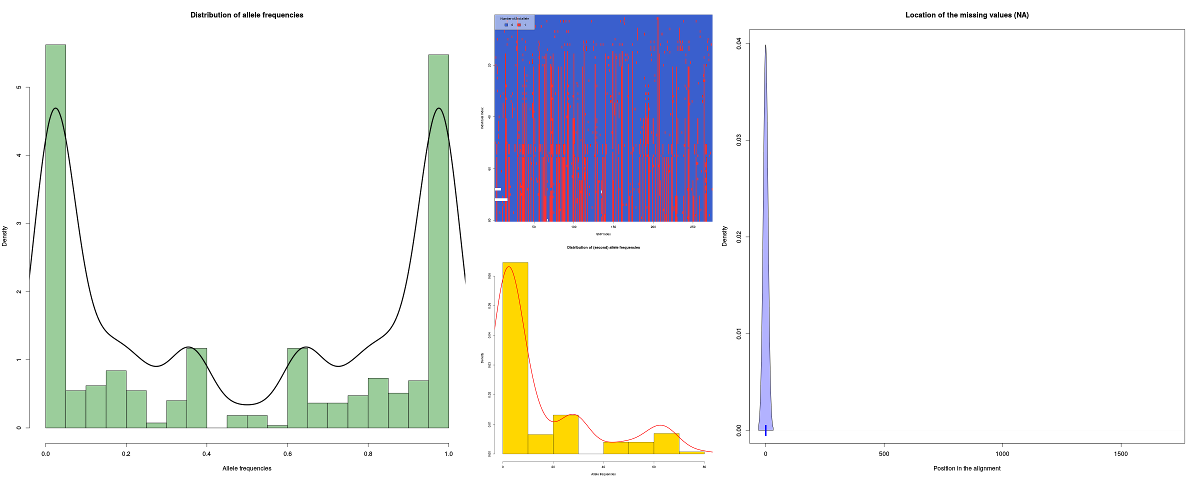
\includegraphics[width=\textwidth]{flu_alleles.png}
\end{frame}

\subsection{PCA and NJ}

\begin{frame}[fragile]{PCA, NJ and genlight objects}
  \begin{spluscode}
    usflu.pca <- glPca(x=usflu.genlight, center=TRUE, scale=FALSE,
      loadings=TRUE) # Select number of retained PC axes, about 10 here
    # Plot PCA
    scatter.glPca(x=usflu.pca, posi="bottomright")
    title("PCA of the US influenza data")
    # Coloured plot
    colorplot(usflu.pca$scores, usflu.pca$scores, transp=TRUE, cex=4)
    title("PCA of the US influenza data")
    abline(h=0, v=0, col="grey")
    add.scatter.eig(usflu.pca[["eig"]][1:40], 2, 1, 2, posi="topright",
      inset=0.05, ratio=0.3)
    # Calculate phylogenetic tree
    usflu.tree.genlight <- nj(dist(as.matrix(usflu.genlight)))
    # Plot colored phylogenetic tree
    plot.phylo(x=usflu.tree.genlight, typ="fan", show.tip=FALSE)
    tiplabels(pch=20, col=num2col(usflu.annot[["year"]],
      col.pal=usflu.pal), cex=4)
    title("NJ tree of the US influenza data")
  \end{spluscode}
\end{frame}

\begin{frame}{PCA, NJ and genlight objects}
  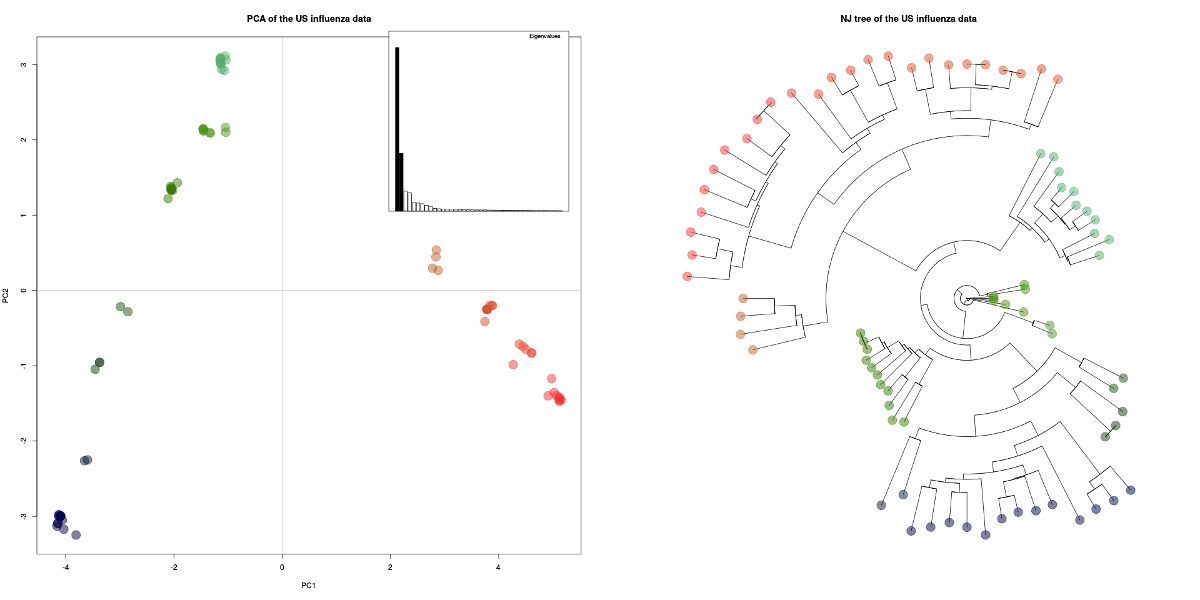
\includegraphics[width=\textwidth]{flu_pcoa_nj.png}
\end{frame}

\section{Spatial analysis}

\begin{frame}{Short overview of spatial genetics (in R)}{Basic approaches}
  \begin{itemize}
    \item Moran's~\textit{I} -- several implementations (here as basic autocorrelation index, in sPCA and in Monmonier's algorithm), generally it is autocorrelation coefficient with broader use
    \item Mantel test -- several implementations, popular, although recently criticized as biologically irrelevant, generally correlation of two matrices (here genetic and geographical)
    \item Bayesian clustering using geographical information as a~proxy and showing results in geographical context (here as implemented in Geneland)
    \item There are unlimited possibilities with connections with GIS software -- check specialized courses and literature
  \end{itemize}
\end{frame}

\subsection{Moran's~I}

\begin{frame}{Moran's~\textit{I}}
  \begin{multicols}{2}
    \begin{itemize}
      \item ``Only'' autocorrelation index -- no genetic/evolutionary model involved -- sometimes criticized as biologically irrelevant mechanism
      \item This (or similar) approach can be used to test correlation between another characteristics (typically used in ecology)
      \item Calculations are done according to connectivity network connecting individuals/populations (created by \texttt{chooseCN}) -- carefully check its options and try several parameters
      \item Pay attention which hypothesis is tested (i.e. if lower, greater or two-sided) -- similar to T-test
    \end{itemize}
    \begin{center}
      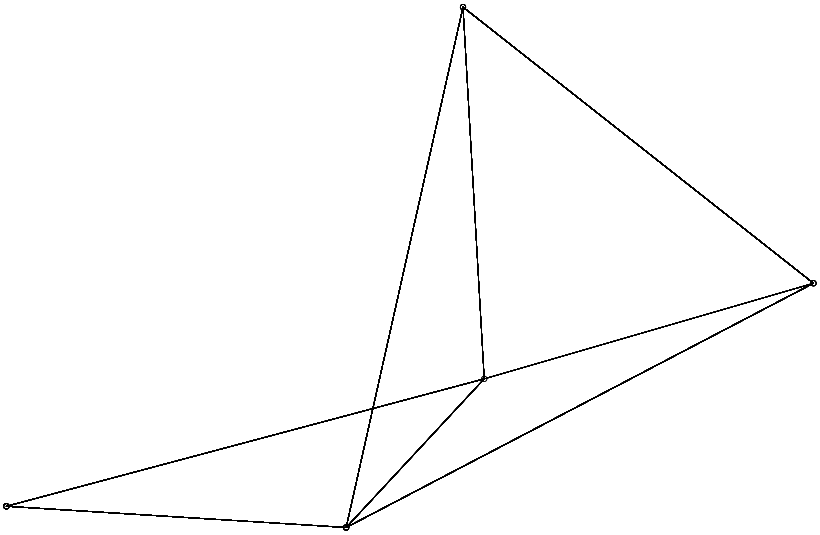
\includegraphics[width=4.5cm]{choosecn.png}
    \end{center}
  \end{multicols}
\end{frame}

\begin{frame}[fragile]{Calculation of Moran's \textit{I} I}
  \begin{spluscode}
    # Load required library
    library(spdep)
    # Creates connection network
    hauss.connectivity <- chooseCN(xy=hauss.genind$other$xy, type=5,
      d1=0, d2=1, plot.nb=TRUE, result.type="listw", edit.nb=FALSE)
    hauss.connectivity
    # Test of Moran's I for 1st PCoA axis
    # Results can be checked against permuted values of moran.mc()
    moran.test(x=hauss.pcoa[["li"]][,1], listw=hauss.connectivity,
      alternative="greater", randomisation=TRUE)
    Moran's I test under randomisation
    data:  hauss.pcoa$li[, 1]
    weights: hauss.connectivity
    Moran I statistic standard deviate = -18.514, p-value = 1
    alternative hypothesis: greater
    sample estimates:
    Moran I statistic       Expectation          Variance
        -0.5232003724     -0.0217391304      0.0007336276
   \end{spluscode}
\end{frame}

\begin{frame}[fragile]{Calculation of Moran's \textit{I} II}
  \begin{spluscode}
    # Test of Moran's I for 1st PCoA axis
    hauss.pcoa1.mctest <- moran.mc(x=hauss.pcoa$li[,1],
      listw=hauss.connectivity, alternative="greater", nsim=1000)
    hauss.pcoa1.mctest
    # Output:
      Monte-Carlo simulation of Moran I
    data:  hauss.pcoa$li[, 1] 
    weights: hauss.connectivity  
    number of simulations + 1: 1001 
    statistic = -0.5163, observed rank = 1, p-value = 0.999
    alternative hypothesis: greater
    # Plot the results
    plot(hauss.pcoa1.mctest) # Plot of densitiy of permutations
    moran.plot(x=hauss.pcoa$li[,1], listw=hauss.connectivity) # PC plot
  \end{spluscode}
\end{frame}

\begin{frame}{Moran's~\textit{I} for our 1$^{st}$ axis isn't significant}
  \begin{center}
    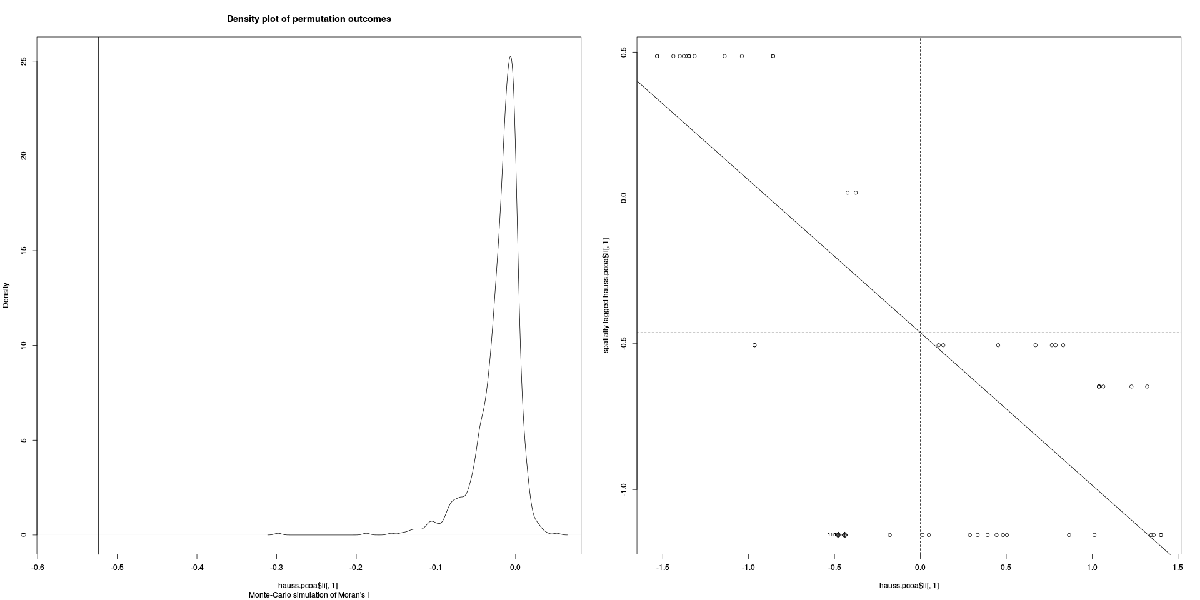
\includegraphics[width=\textwidth-1.5cm]{moran1.png}
  \end{center}
  \begin{itemize}
    \item Tested hypothesis ``greater'' -- \textbf{no} significant \textbf{positive} autocorrelation
    \item If testing for hypothesis ``less'' -- significant \textbf{negative} autocorrelation -- individuals are significantly different
  \end{itemize}
\end{frame}

\begin{frame}[fragile]{Calculation of Moran's \textit{I} (2$^{nd}$ axis)}
  \begin{spluscode}
    # Test of Moran's I for 2nd PCoA axis
    moran.test(x=hauss.pcoa$li[,2], listw=hauss.connectivity,
      alternative="greater", randomisation=TRUE)
    hauss.pcoa2.mctest <- moran.mc(x=hauss.pcoa$li[,2],
      listw=hauss.connectivity, alternative="greater", nsim=1000)
    hauss.pcoa2.mctest
    # Output
    Monte-Carlo simulation of Moran's I
    data:  hauss.pcoa$li[, 2] 
    weights: hauss.connectivity  
    number of simulations + 1: 1001 
    statistic = 0.0545, observed rank = 1001, p-value = 0.000999
    alternative hypothesis: greater
    # Plot the results
    plot(hauss.pcoa2.mctest) # Plot of densitiy of permutations
    moran.plot(x=hauss.pcoa$[,2], listw=hauss.connectivity) # PC plot
  \end{spluscode}
\end{frame}

\begin{frame}{Second axis is surprisingly significant}
  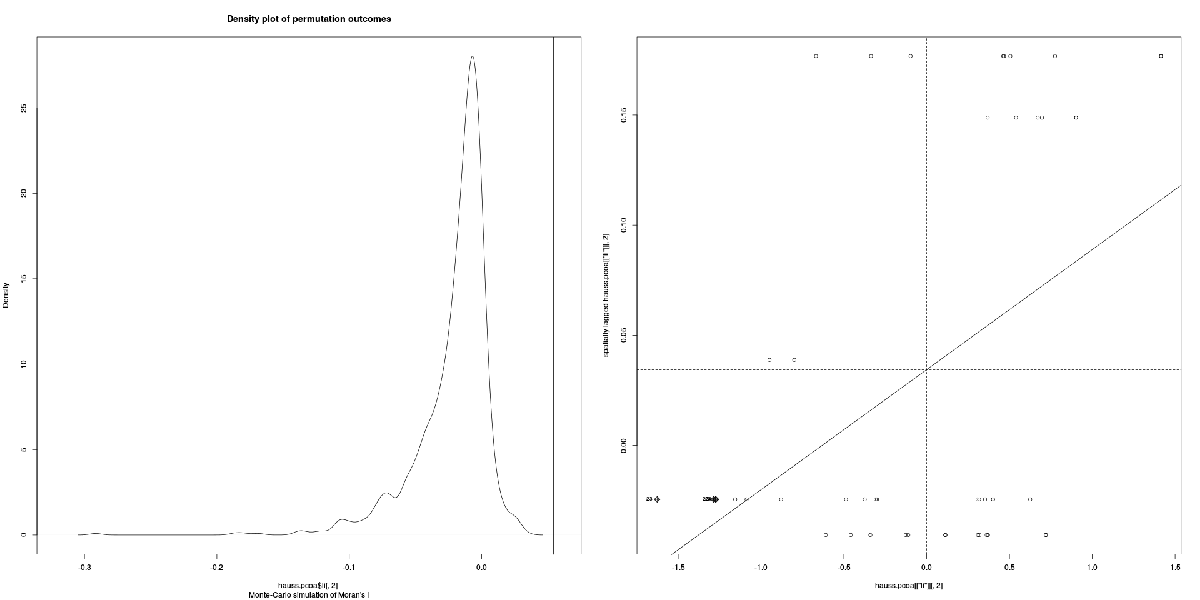
\includegraphics[width=\textwidth]{moran2.png}
  \begin{itemize}
    \item Tested hypothesis ``greater'' -- there \textbf{is} significant positive autocorrelation -- individuals are genetically similar over space
  \end{itemize}
\end{frame}

\subsection{sPCA}

\begin{frame}[fragile]{Spatial Analysis of Principal Components (sPCA)}
  \begin{itemize}
    \item Implemented in adegenet, see \texttt{adegenetTutorial("spca")}
    \item Analyzes matrix of relative allele frequencies of genotypes/populations and spatial weighting matrix
    \item The geographical matrix is usually (as for Moran's~\textit{I}) created by \texttt{chooseCN()} -- creates connectivity network among entities (genotypes/populations) -- spatial coordinates are not directly used
    \item When using \texttt{chooseCN()}, look at the documentation and try various methods with changing settings to see differences
  \end{itemize}
  \begin{spluscode}
    data(rupica) # Loads adegenet's training dataset
                 # Rupicapra rupicapra from French Alps
    # Try various settings for chooseCN (type=X) - type 1-4 as there
    # are identical coordinates (multiple sampling from same locality)
    chooseCN(xy=rupica$other$xy, ask=TRUE, type=5/6/7, plot.nb=TRUE,
      edit.nb=FALSE, ...) # Play with settings little bit...
    ?chooseCN # See for more details - select the best "type" for your data
  \end{spluscode}
\end{frame}

\begin{frame}[fragile]{Calculations of sPCA}
  \begin{spluscode}
    hauss.spca <- spca(obj=hauss.genind, cn=hauss.connectivity,
      scale=TRUE, scannf=TRUE)
    # Plot eigenvalues of sPCA - global vs. local structure
    barplot(height=hauss.spca$eig, main="Eigenvalues of sPCA",
      col=spectral(length(hauss.spca$eig)))
    legend("topright", fill=spectral(2), leg=c("Global structures",
      "Local structures")) # Add legend
    abline(h=0,col="grey") # Add line showing zero
    print.spca(hauss.spca) # Information about sPCA
    summary.spca(hauss.spca) # Summary of sPCA results
    # Shows connectivity network, 3 different scores
    # barplot of eigenvalues and eigenvalues decomposition
    plot.spca(hauss.spca)
    colorplot.spca(hauss.spca, cex=3) # Display of scores in color canals
    title("sPCA - colorplot of PC 1 and 2 (lagged scores)", line=1, cex=1.5)
    # Spatial and variance components of the eigenvalues
    screeplot.spca(x=hauss.spca, main=NULL)
  \end{spluscode}
\end{frame}

\begin{frame}{sPCA outputs I}
  \begin{center}
    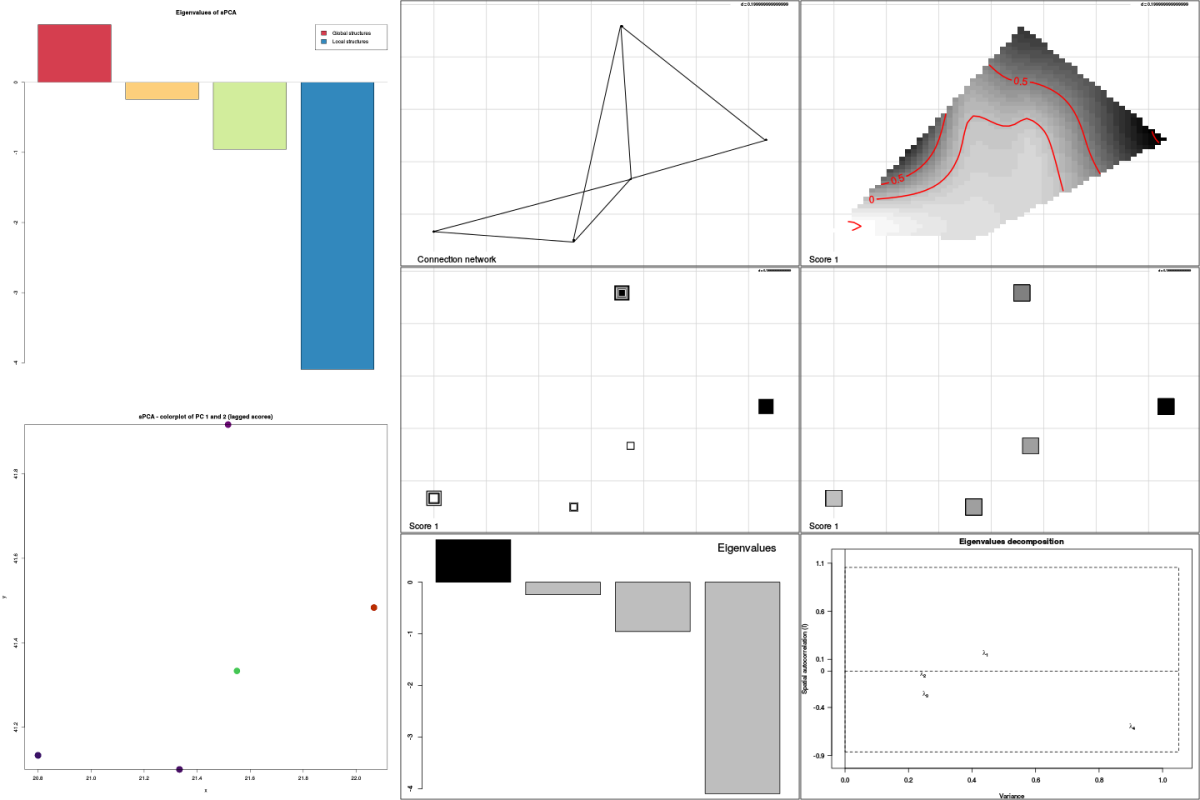
\includegraphics[width=\textwidth-1.5cm]{spca.png}
  \end{center}
\end{frame}

\begin{frame}[fragile]{Map of genetic clines}
  \begin{spluscode}
    library(akima) # It is needed for manipulation with coordinates
    # Transform the coordinates
    hauss.spca.temp <- interp(other(hauss.genind)$xy[,1],
      other(hauss.genind)$xy[,2], hauss.spca$ls[,1],
      xo=seq(min(other(hauss.genind)$xy[,1]),
      max(other(hauss.genind)$xy[,1]), le=200),
      yo=seq(min(other(hauss.genind)$xy[,2]),
      max(other(hauss.genind)$xy[,2]), le=200), duplicate="median")
    # For 1st axis
    image(x=hauss.spca.temp, col=spectral(100))
    s.value(dfxy=hauss.genind$other$xy, z=hauss.pcoa$li[,1],
      add.p=TRUE, csize=0.5, sub="PCoA - first PC", csub=2,
      possub="topleft")
    # For 2nd axis
    image(x=hauss.spca.temp, col=spectral(100))
    s.value(dfxy=hauss.genind$other$xy, z=hauss.pcoa[["li"]][,2],
      add.p=TRUE, csize=0.5, sub="PCoA - second PC", csub=2,
      possub="topleft")
  \end{spluscode}
\end{frame}

\begin{frame}[fragile]{sPCA outputs II}
  \begin{spluscode}
    # Interpolated lagged score on a map
    hauss.spca.annot <- function() {
      title("sPCA - interpolated map of individual scores")
      points(other(hauss.genind)$xy[,1], other(hauss.genind)$xy[,2])
      }
    filled.contour(hauss.spca.temp, color.pal=colorRampPalette(
      lightseasun(100)), pch=20, nlevels=100, key.title=title("Lagged\n
      score 1"), plot.title=hauss.spca.annot())
  \end{spluscode}

  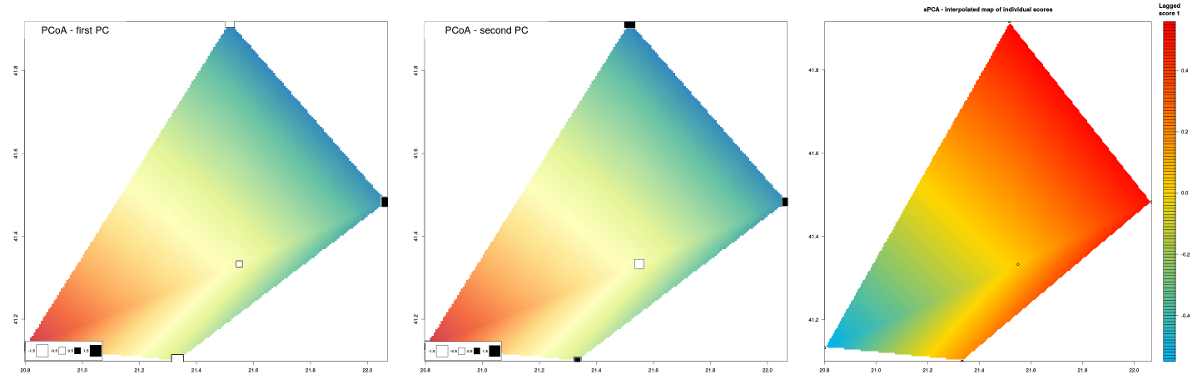
\includegraphics[width=\textwidth]{spca-pc.png}
\end{frame}

\begin{frame}[fragile]{Loading plots -- which alleles contribute the most?}
  \begin{spluscode}
    hauss.spca.loadings <- hauss.spca[["c1"]][,1]^2
    names(hauss.spca.loadings) <- rownames(hauss.spca$c1)
    loadingplot(x=hauss.spca.loadings, xlab="Alleles", ylab="Weight of the
      alleles", main="Contribution of alleles to the first sPCA axis")
    boxplot(formula=hauss.spca.loadings~hauss.genind$loc.fac, las=3,
      ylab="Contribution", xlab="Marker", main="Contribution by markers
      into the first global score", col="grey")
  \end{spluscode}
  \vfil
  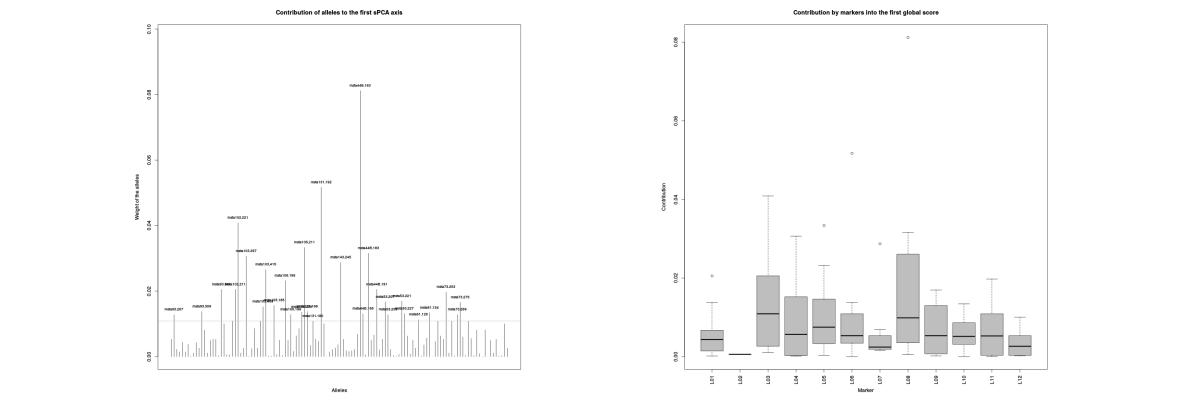
\includegraphics[width=\textwidth]{spca-loading.png}
  \vfill
\end{frame}

\subsection{Monmonier}

\begin{frame}[fragile]{Monmonier's algorithm -- genetic boundaries}
  \begin{itemize}
    \item Finds boundaries of maximum differences between contiguous polygons of a~tessellation
    \item Detects genetic boundaries among georeferenced genotypes (or populations)
    \item For more information see \texttt{adegenetTutorial("basics")}
    \item Requires every point to have unique coordinates -- in case of population data it is better to work with populations, not individuals (but it is not ideal)
    \item It uses \href{https://en.wikipedia.org/wiki/Voronoi_diagram}{Voronoi tessellation}
  \end{itemize}
  \begin{spluscode}
    # Calculates Monmonier's function (for threshold use 'd')
    hauss.monmonier <- monmonier(xy=hauss.genpop$other$xy, dist=
      dist(hauss.genpop@tab), cn=chooseCN(hauss.genpop$other$xy,
      ask=FALSE, type=2, plot.nb=FALSE, edit.nb=FALSE), nrun=1)
    coords.monmonier(hauss.monmonier) # See result as text
  \end{spluscode}
\end{frame}

\begin{frame}{Voronoi tessellation}
  \begin{multicols}{2}
    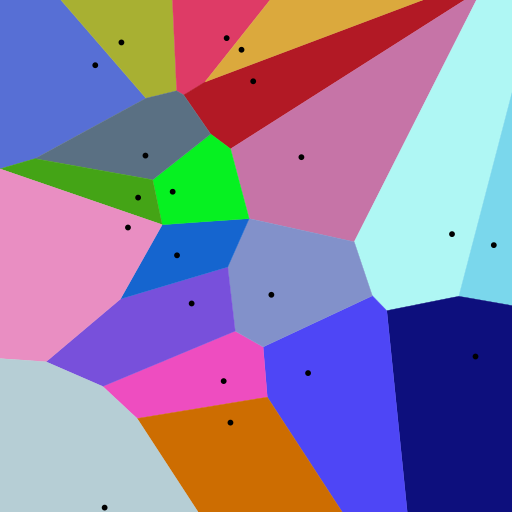
\includegraphics[height=5.5cm]{voronoi_diagram.png}
    \begin{itemize}
      \item In simplest case, all points have certain area and all points within this area are closer to the respective ``main'' point than to any other ``neighbor'' point
      \item Extreme differences among size of areas make computational problems and results are unstable -- this typically occurs when calculations are done on individual level an there are large distances among populations
    \end{itemize}
  \end{multicols}
\end{frame}

\begin{frame}[fragile]{Plot genetic boundaries}
\begin{multicols}{2}
  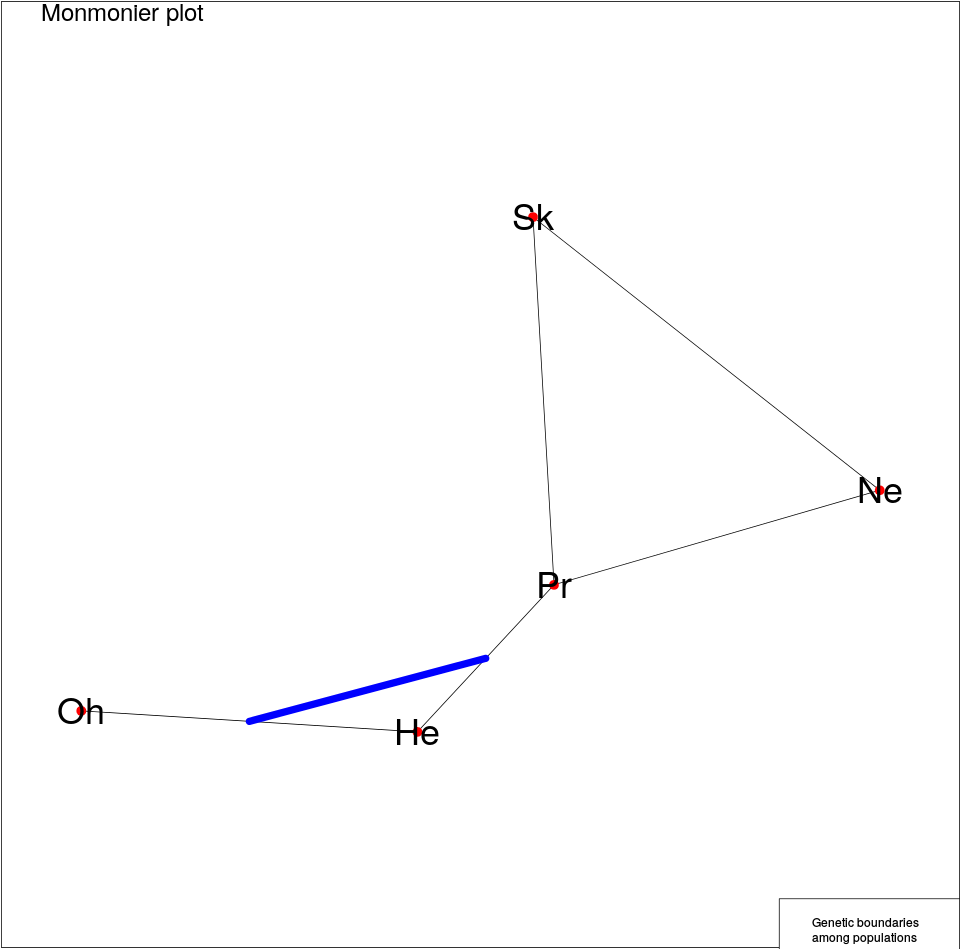
\includegraphics[height=5.5cm]{monmonier.png}
  \begin{spluscode}
    plot.monmonier(hauss.monmonier,
      add.arrows=FALSE, bwd=10,
      sub="Monmonier plot", csub=2)
    points(hauss.genpop$other$xy,
      cex=2.5, pch=20, col="red")
    text(x=hauss.genpop$other$xy$lon,
      y=hauss.genpop$other$xy$lat,
      labels=popNames(hauss.genpop),
      cex=3)
    legend("bottomright",
      leg="Genetic boundaries\n
      among populations")
    # See ?points, ?text and ?legend
  \end{spluscode}
\end{multicols}
\end{frame}

\begin{frame}[fragile]{Monmonier notes}
  \begin{itemize}
    \item Sometimes it is needed to get rid of random noise in data. To do so use as parameter \texttt{dist} of \texttt{monmonier()} table from PCA (\texttt{pcaObject\$li}):
  \end{itemize}
  \begin{spluscode}
    monmonier(..., dist=dudi.pco(d=dist(x=GenindObject$tab),
      scannf=FALSE, nf=1)$li, ...)
  \end{spluscode}
  \begin{itemize}
    \item Generally (when dataset is bigger and more diverse) it is recommended to run it several times (parameter \texttt{nrun}) -- there will be several iterations
    \item See \texttt{?plot.monmonier} for various graphical parameters to customize the plot
    \item Use \texttt{points()} to add for example colored symbols of samples and/or \texttt{text()} to add text labels
  \end{itemize}
\end{frame}

\subsection{Mantel test}

\begin{frame}{Mantel test}
  \begin{itemize}
    \item Originally created for biomedicine to test correlation between treatment and diseases
    \item ``Only'' correlation of two matrices -- no biologically relevant underlying model -- because of that it is heavily criticized (mainly in ecology)
    \item It is universal method usable for plenty of tasks
    \item Test of spatial and genetic relationships is probably one of few biologically relevant applications
    \item Package vegan (set of ecological tools) has implementation to test genetic similarity in various distance classes -- not only overall result -- very useful
  \end{itemize}
\end{frame}

\begin{frame}[fragile]{Mantel test -- isolation by distance}
  \begin{spluscode}
    # Geographical distance
    hauss.gdist <- dist(x=hauss.genind$other$xy, method="euclidean",
      diag=TRUE, upper=TRUE)
    # Mantel test
    hauss.mantel <- mantel.randtest(m1=hauss.dist, m2=hauss.gdist,
      nrepet=1000)
    hauss.mantel # See text output
    plot(hauss.mantel, nclass=30)
    # Libraries required by mantel.correlog:
    library(permute)
    library(lattice)
    library(vegan)
    # Different implementation of Mantel test testing distance classes
    hauss.mantel.cor <- mantel.correlog(D.eco=hauss.dist,D.geo=hauss.gdist,
      XY=NULL, n.class=0, break.pts=NULL, cutoff=FALSE, r.type="pearson",
      nperm=1000, mult="holm", progressive=TRUE)
    # See results for respective classes
    hauss.mantel.cor
    summary(hauss.mantel.cor)
  \end{spluscode}
\end{frame}

\begin{frame}[fragile]{Mantel test outputs -- strongly significant}
\begin{multicols}{2}
  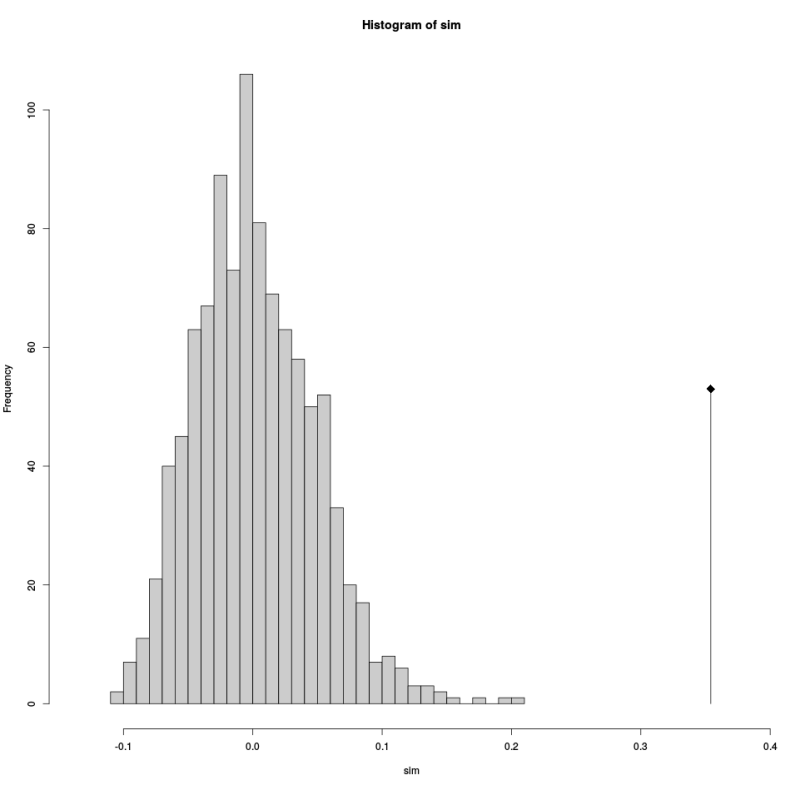
\includegraphics[height=6cm]{mantel.png}
  \begin{spluscode}
    hauss.mantel # See output
    Monte-Carlo test
    Call: mantel.randtest(m1 =
      hauss.dist, m2 =
      hauss.gdist, nrepet = 1000)
    Observation: 0.35409
    Based on 1000 replicates
    Simulated p-value: 0.000999001
    Alternative hypothesis: greater
      Std.Obs Expectation  Variance
    7.61967545 0.001687140 0.0021389
  \end{spluscode}
  \vfill
  \begin{spluscode}
    # Plot correlogram (next slide)
    plot(hauss.mantel.cor)
  \end{spluscode}
\end{multicols}
\end{frame}

\begin{frame}{Plot of Mantel Correlogram Analysis}
  \vfil
  \begin{center}
    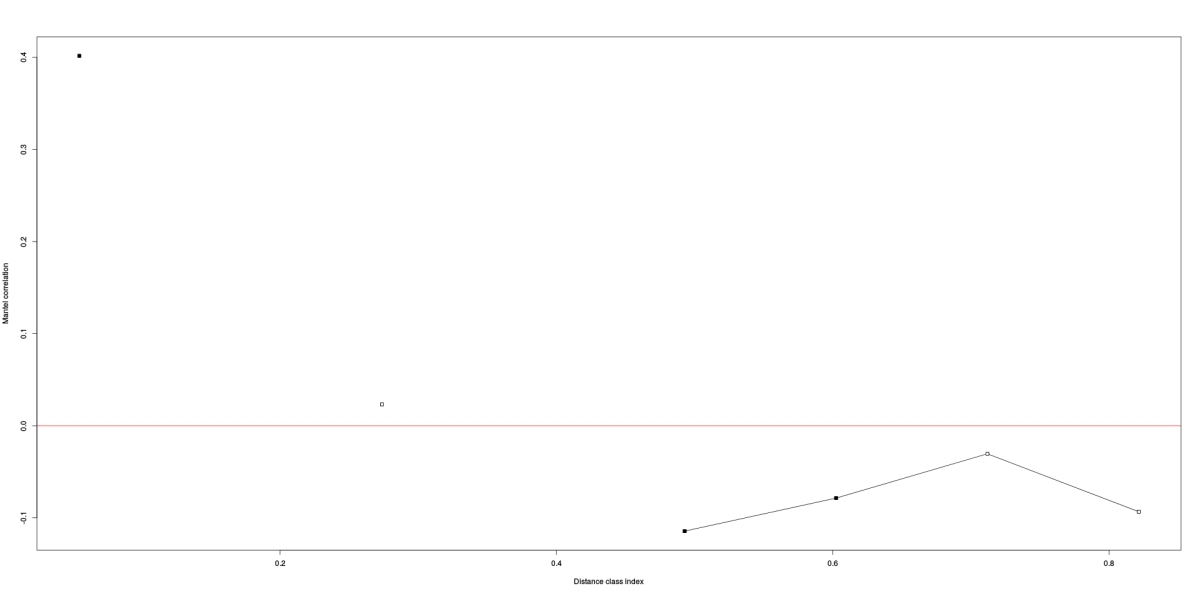
\includegraphics[width=\textwidth-1cm]{mantel-cor.png}
  \end{center}
  \vfil
  Correlation (genetic similarity) in several distance classes (positive \textbf{[up]} in short distance \textbf{[left]}, negative \textbf{[down]} in long \textbf{[right]}; \textbf{[full]} -- significant, \textbf{[empty]} -- not significant) -- see \texttt{?mantel.correlog} for details
  \vfill
\end{frame}

\begin{frame}[fragile]{Mantel correlogram -- text output}
  \begin{spluscode}
    hauss.mantel.cor # See the text output:
    Mantel Correlogram Analysis
    Call:
    mantel.correlog(D.eco = hauss.dist, D.geo = hauss.gdist, XY = NULL,
     n.class = 0, break.pts = NULL, cutoff = FALSE, r.type = "pearson",
     nperm = 1000, mult = "holm", progressive = TRUE) 
            class.index     n.dist Mantel.cor Pr(Mantel) Pr(corrected)
    D.cl.1     0.054757 532.000000   0.409545     0.0010      0.000999 ***
    D.cl.2     0.164271   0.000000         NA         NA            NA
    D.cl.3     0.273784  52.000000   0.028055     0.2797      0.279720
    D.cl.4     0.383298   0.000000         NA         NA            NA
    D.cl.5     0.492812 466.000000  -0.097214     0.0160      0.031968 *
    D.cl.6     0.602325  36.000000  -0.086288     0.0140      0.041958 *
    D.cl.7     0.711839 108.000000  -0.044109     0.1568      0.313686
    D.cl.8     0.821353 458.000000  -0.095780     0.0100      0.049950 *
    ...        ...      ...         ...           ...         ...
    ---
    Signif. codes:  0 ‘***’ 0.001 ‘**’ 0.01 ‘*’ 0.05 ‘.’ 0.1 ‘ ’ 1
  \end{spluscode}
\end{frame}

\subsection{Geneland}

\begin{frame}[fragile]{About Geneland}
\begin{multicols}{2}
  \begin{itemize}
    \item Works with haploid and diploid codominant markers (microsatellites or SNPs)
    \item Spatially explicit Bayesian clustering
    \item Produces maps of distribution of inferred genetic clusters
    \item Relative complicated tool with various modeling options
  \end{itemize}
  \columnbreak
  \begin{spluscode}
    # Load needed libraries
    library(PBSmapping)
    library(RandomFields)
    library(fields)
    library(spam)
    library(grid)
    library(maps)
    library(tcltk)
    library(Geneland)
    # Graphical interface is available
    # we will use only command line...
    Geneland.GUI()
  \end{spluscode}
\end{multicols}
For more information see \url{https://www2.imm.dtu.dk/~gigu/Geneland/}
\end{frame}

\begin{frame}{Geneland GUI}
  \begin{itemize}
    \item Some tasks are easier in GUI, some in command line\ldots
    \item Command line is great for its repeatability\ldots
    \item Always read manual! It is not the simplest tool\ldots
  \end{itemize}
  \begin{center}
    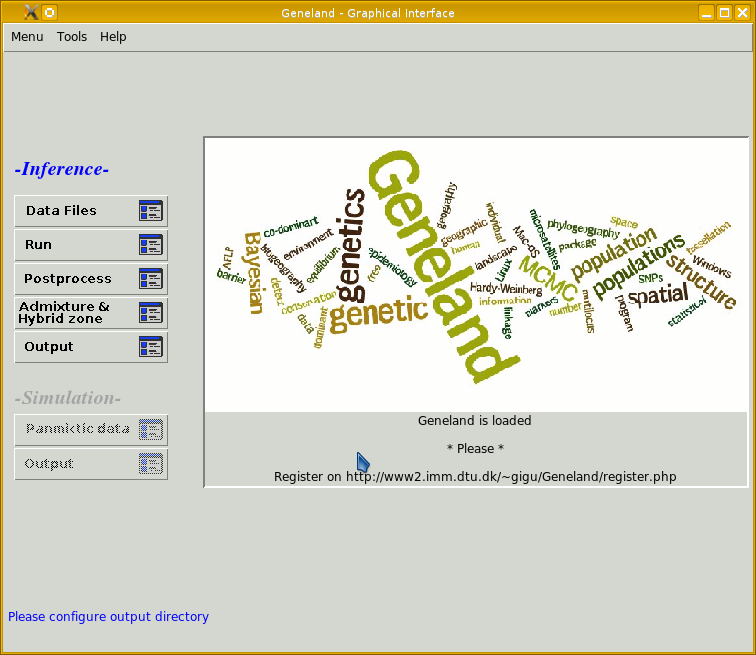
\includegraphics[height=5cm]{geneland_gui.png}
  \end{center}
\end{frame}

\begin{frame}[fragile]{Loading and conversions of coordinates}
  \begin{spluscode}
    # Geneland requires specific coordinate space
    # hauss.cord is DF, we need just plain matrix
    hauss.geneland.coord <- as.matrix(hauss.coord)
    colnames(hauss.geneland.coord) <- c("X", "Y")
    attr(hauss.geneland.coord, "projection") <- "LL"
    attr(hauss.geneland.coord, "zone") <- NA
    hauss.geneland.coord.utm <- convUL(hauss.geneland.coord)
    dim(hauss.geneland.coord)
    hauss.geneland.coord
    dim(hauss.geneland.coord.utm)
    hauss.geneland.coord.utm # Final coordinates
    # Load data (only haploid or diploid data are supported)
    # only plain table with alleles
    hauss.geneland.data <- read.table(file=
      "https://soubory.trapa.cz/rcourse/haussknechtii_geneland.txt",
      na.string="-999", header=FALSE, sep="\t")
    dim(hauss.geneland.data)
    hauss.geneland.data
  \end{spluscode}
\end{frame}

\begin{frame}[fragile]{Before running MCMC}
  \begin{multicols}{2}
    \begin{itemize}
      \item Monte Carlo Markov Chains (MCMC) require usually millions of generations (iterations, \texttt{nit)} to find optimal solution
      \item Beginning ($\sim$10-20\%) of the steps (\texttt{burnin}) use to be very unstable and useless for following analyses and it is discarded
      \item Geneland allows to set density of sampling among generations (\texttt{thinning}) -- it is not necessary to sample every generation
      \item Within millions of generations we can sample every 1000-10000$^{th}$ generation
      \item Denser sampling produces smoother data, but can consume too much disk space\ldots
    \end{itemize}
    \vfill
    Directory structure for Geneland:
    \vfil
    \begin{center}
      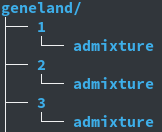
\includegraphics[width=2cm]{genelad_dirs.png}
    \end{center}
    \vfil
  \end{multicols}
\end{frame}

\begin{frame}[fragile]{Settings and running MCMC}
  \begin{spluscode}
    hauss.geneland.nrun <- 5 # Set number of independent runs
    hauss.geneland.burnin <- 100 # Set length of burnin chain
    hauss.geneland.maxpop <- 10 # Set maximal K (number of populations)
    # FOR loop will run several independent runs and produce output maps
    # of genetic clusters - outputs are written into subdirectory within
    # geneland directory (this has to exist prior launching analysis)
    for (hauss.geneland.irun in 1:hauss.geneland.nrun) {
      hauss.geneland.path.mcmc <- paste("geneland/", hauss.geneland.irun,
        "/", sep="") # paste is good especially for joining several texts
      # On Windows, remove following line and create subdirectories from
      # 1 to max K manually (creating subdirs in Windows is complicated)
      system(paste("mkdir ", hauss.geneland.path.mcmc)) # Creates subdirs
      # Inference - MCMC chain - see ?MCMC for details
      MCMC(coordinates=hauss.geneland.coord.utm, geno.dip.codom=
        hauss.geneland.data, path.mcmc=hauss.geneland.path.mcmc,
        delta.coord=0.001, varnpop=TRUE, npopmin=1, npopmax=
        hauss.geneland.maxpop, nit=10000, thinning=10,
        freq.model="Uncorrelated", spatial=TRUE)
      # For loop continues on next slide
  \end{spluscode}
\end{frame}

\begin{frame}[fragile]{Running MCMC}
  \begin{spluscode}
      # Start of FOR loop is on previous page
      # In practice set much higher number of iterations (nit),
      # appropriate sampling (thinning) and longer burnin
      # Post-process chains
      PostProcessChain(coordinates=hauss.geneland.coord.utm,
        path.mcmc=hauss.geneland.path.mcmc, nxdom=500, nydom=500,
        burnin=hauss.geneland.burnin)
      # Output
      # Simulated number of populations
      Plotnpop(path.mcmc=hauss.geneland.path.mcmc, printit=TRUE,
        file=paste(hauss.geneland.path.mcmc, "/geneland-number_of_clusters
        .pdf", sep=""), format="pdf", burnin=hauss.geneland.burnin)
      dev.off() # We must close graphical device manually
      # Map of estimated population membership
      PosteriorMode(coordinates=hauss.geneland.coord.utm, 
        path.mcmc=hauss.geneland.path.mcmc, printit=TRUE, format="pdf",
        file=paste(hauss.geneland.path.mcmc,"/geneland-map.pdf", sep=""))
      dev.off() # We must close graphical device manually
      } # End of FOR loop from previous slide
  \end{spluscode}
\end{frame}

\begin{frame}[fragile]{Estimate F$_{ST}$}
  \begin{spluscode}
    # Prepare list to record values of Fst for all runs
    hauss.geneland.fstat <- list()
    # Estimate Fst
    for (hauss.geneland.irun in 1:hauss.geneland.nrun) {
      hauss.geneland.path.mcmc <- paste("geneland/",
      hauss.geneland.irun, "/", sep="")
      # F-statistics - Fis and Fst
      hauss.geneland.fstat[[hauss.geneland.irun]] <- Fstat.output(
        coordinates=hauss.geneland.coord.utm,
        genotypes=hauss.geneland.data,
        burnin=hauss.geneland.burnin, ploidy=2,
        path.mcmc=hauss.geneland.path.mcmc)
      }
      # Print Fst output
      hauss.geneland.fstat
  \end{spluscode}
\end{frame}

\begin{frame}[fragile]{MCMC inference under the admixture model}
  \begin{spluscode}
    for (hauss.geneland.irun in 1:hauss.geneland.nrun) {
      hauss.geneland.path.mcmc <- paste("geneland/",
        hauss.geneland.irun, "/", sep="")
      hauss.geneland.path.mcmc.adm <- paste(hauss.geneland.path.mcmc,
        "admixture", "/", sep="")
      # On Windows, remove following line of code and create in each
      # result directory (from 1 to max K) new subdirectory "admixture"
      # (creating subdirs in Windows is complicated)
      system(paste("mkdir ", hauss.geneland.path.mcmc.adm))
      HZ(coordinates=hauss.geneland.coord.utm, geno.dip.codom=
        hauss.geneland.data, path.mcmc.noadm=hauss.geneland.path.mcmc,
        nit=10000, thinning=10,
        path.mcmc.adm=hauss.geneland.path.mcmc.adm)
      }
  \end{spluscode}
  \begin{itemize}
    \item Currently, there is no much use for admixture results, at lest not without extra work\ldots
  \end{itemize}
\end{frame}

\begin{frame}[fragile]{Produce maps of respective inferred clusters}
  \begin{spluscode}
    for (hauss.geneland.irun in 1:hauss.geneland.nrun) {
      hauss.geneland.path.mcmc <- paste("geneland/",
        hauss.geneland.irun, "/", sep="")
      # Maps - tessellations
      PlotTessellation(coordinates=hauss.geneland.coord.utm,
        path.mcmc=hauss.geneland.path.mcmc, printit=TRUE,
        path=hauss.geneland.path.mcmc)
      for (hauss.geneland.irun.img in 1:hauss.geneland.maxpop) {
        dev.off() } # We must close graphical device manually
      }
  \end{spluscode}
  \begin{itemize}
    \item Maps are produced as PS (PostScript) files in output directories
    \item Not every graphical software can handle PS (try for example \href{https://www.gimp.org/}{GIMP})
    \item There are as many plots as was maximal K, but only those up to inferred number of clusters have some content (the others are empty)
  \end{itemize}
\end{frame}

\begin{frame}[fragile]{Determine which run is the best}
  \begin{spluscode}
    # Calculate average posterior probability
    hauss.geneland.lpd <- rep(NA, hauss.geneland.nrun)
    for (hauss.geneland.irun in 1:hauss.geneland.nrun) {
      hauss.geneland.path.mcmc <- paste("geneland/",
        hauss.geneland.irun, "/", sep="")
      hauss.geneland.path.lpd <- paste(hauss.geneland.path.mcmc,
        "log.posterior.density.txt", sep="")
      hauss.geneland.lpd[hauss.geneland.irun] <- 
        mean(scan(hauss.geneland.path.lpd)[-(1:hauss.geneland.burnin)]) }
    # Sorts runs according to decreasing posterior probability
    # the first one is the best
    order(hauss.geneland.lpd, decreasing=TRUE)
    [1] 5 1 4 3 2 # Run 5 is the best here
    hauss.geneland.lpd # Here the runs are unsorted
    [1] -645.0238 -782.7912 -676.9559 -664.9947 -601.7902 # Run 5 wins
  \end{spluscode}
  \begin{itemize}
    \item We will use figures and F$_{ST}$ outputs only from the best run
    \item It is useful to keep all runs especially for comparison if there are different solutions with similar posterior probability
  \end{itemize}
\end{frame}

\begin{frame}{MCMC chain, number of clusters and their map}{MCMC did not converge yet -- too few generations, the most likely solution is K=4 followed by K=5. Final product is map of distribution of genetic clusters.}
  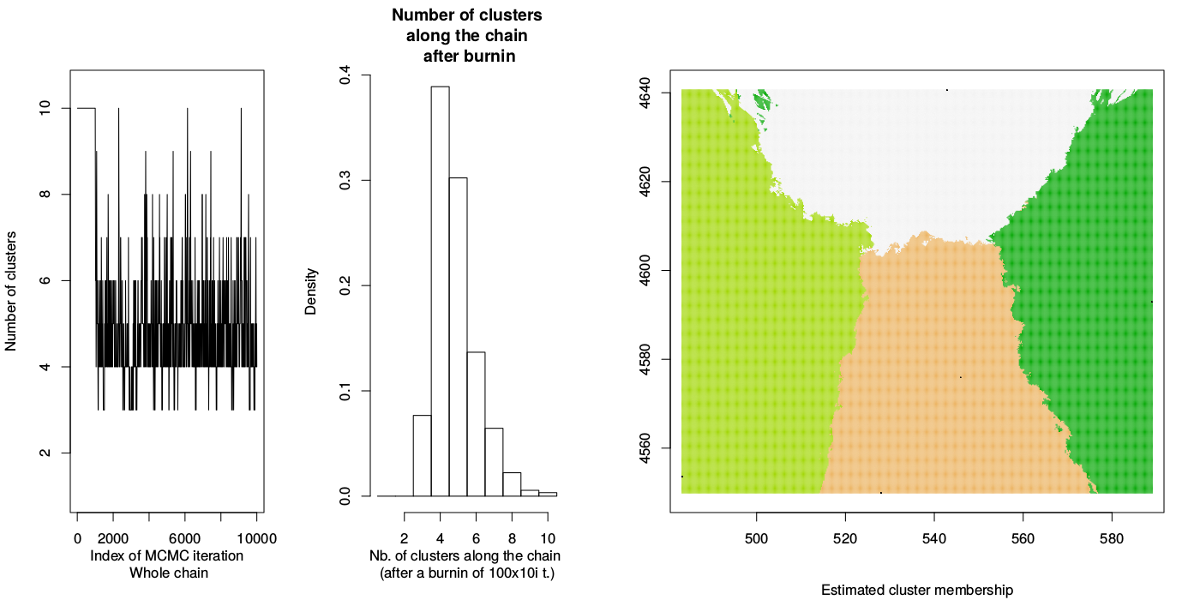
\includegraphics[width=\textwidth]{geneland1.png}
\end{frame}

\begin{frame}{Map of posterior probability of belonging into cluster 1}
  \begin{center}
    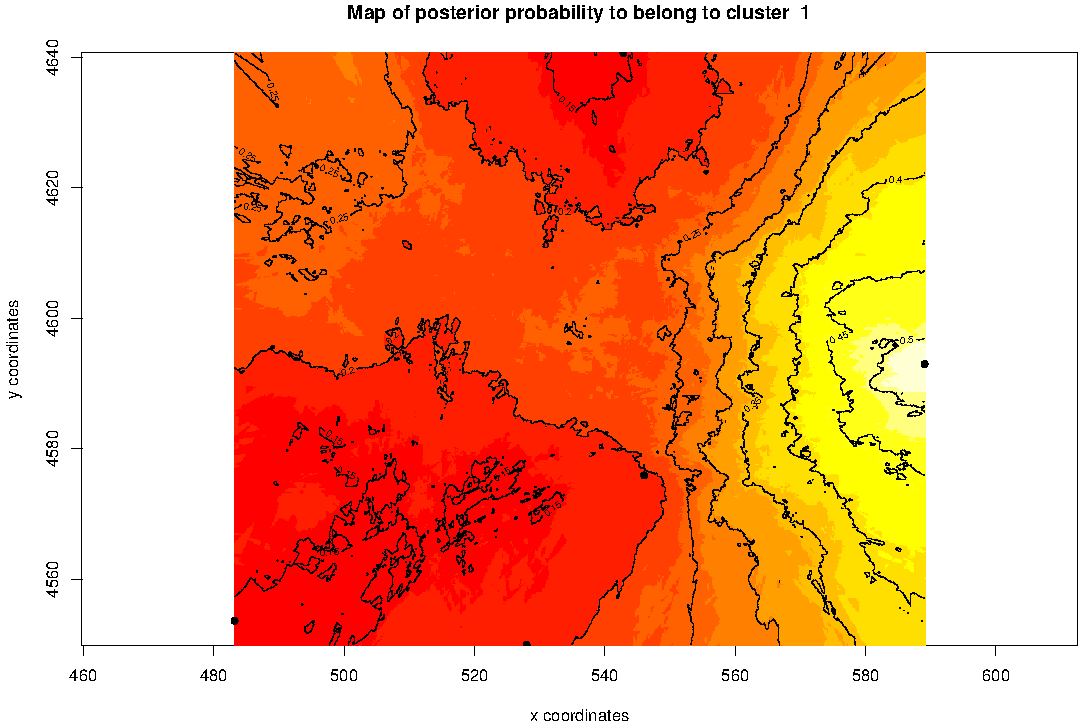
\includegraphics[width=\textwidth-1.5cm]{geneland2.png}
  \end{center}
\end{frame}

\subsection{Plotting maps}

\begin{frame}[fragile]{Very basic mapping in R}
  \begin{spluscode}
    # Load libraries
    library(sp)
    library(rworldmap) # Basic world maps
    library(TeachingDemos) # To be able to move text little bit
    library(RgoogleMaps) # Google and OpenStreetMaps
    # Plot basic map with state boundaries within selected range
    plot(x=getMap(resolution="high"), xlim=c(19, 24), ylim=c(39, 44),
      asp=1, lwd=1.5)
    box() # Add frame around the map
    # Plot location points
    points(x=hauss.genpop@other$xy[["lon"]], y=hauss.genpop@other$xy
      [["lat"]], pch=15:19, col="red", cex=4)
    # Add text descriptions for points. Text is aside and with background
    shadowtext(x=hauss.genpop@other$xy[["lon"]], y=hauss.genpop@other$xy
      [["lat"]], labels=as.vector(popNames(hauss.genind)), col="black",
      bg="white", theta=seq(pi/4, 2*pi, length.out=8), r=0.15,
      pos=c(1, 3, 2, 4, 4), offset=0.75, cex=1.5)
  \end{spluscode}
\end{frame}

\begin{frame}[fragile]{Basic map and Google map}
\begin{multicols}{2}
  \begin{spluscode}
    # Insert legend
    legend(x="topright", inset=1/50,
      legend=c("He", "Oh", "Pr", "Ne",
      "Sk"), col="red", border="black",
      pch=15:19, pt.cex=2, bty="o",
      bg="lightgrey", box.lwd=1.5,
      cex=1.5, title="Populations")
    # Google map is produced into a
    # file. Parameter markers contain
    # data frame with coordinates and
    # possibly with more information
    hauss.gmap <- GetMap(center=
      c(lat=41, lon=21), size=c(640,
      640), destfile="gmap.png",
      zoom=8, markers=hauss.coord,
      maptype="terrain") # Plot saved map:
    PlotOnStaticMap(MyMap=hauss.gmap)
  \end{spluscode}
  \begin{center}
    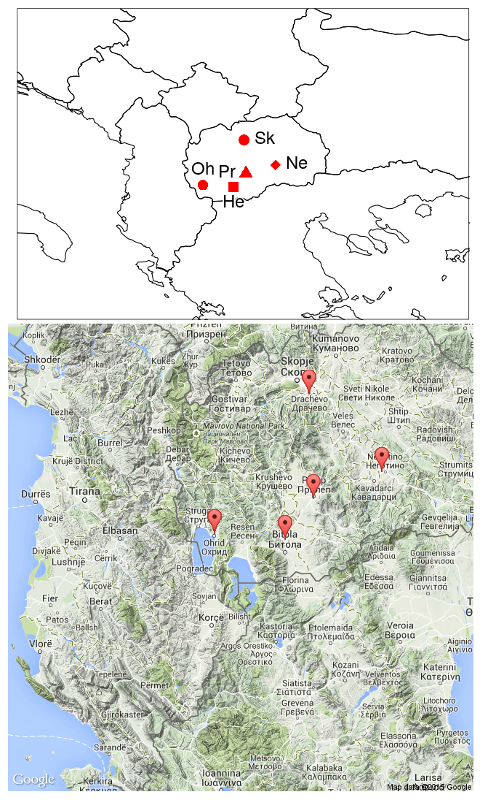
\includegraphics[height=6.5cm]{maps.png}
  \end{center}
\end{multicols}
\end{frame}

\begin{frame}[fragile]{OpenStreetMaps and datasets from mapproj}
  \begin{spluscode}
    # Plot on OpenStreetMaps - server is commonly overloaded and does not
    # respond correctly - in fact, it rarely works...
    GetOsmMap(lonR=c(18, 24), latR=c(39, 44), scale=200000, destfile=
      "osmmap.png", format="png", RETURNIMAGE=TRUE, GRAYSCALE=FALSE,
      NEWMAP=TRUE, verbose=1)
    # Plot on datasets from mapproj package
    library(maps) # Various maping tools (plotting, ...)
    library(mapdata) # More detailed maps, but political boundaries often
           # outdated, see https://cran.r-project.org/web/packages/mapdata/
    library(mapproj) # Convert latitude/longitude into projected coordinates
    # Plot a map, check parameters
    # Check among others "projection" and ?mapproject for its details
    map(database="worldHires", boundary=TRUE, interior=TRUE, fill=TRUE,
      col="lightgrey", plot=TRUE, xlim=c(16, 27), ylim=c(37, 46))
    # If you'd use projection, use mapproject to convert also coordinates!
    # See ?mapproject for details
    points(x=hauss.genpop@other$xy[["lon"]], y=hauss.genpop@other$xy
      [["lat"]], pch=15:19, col="red", cex=3)
  \end{spluscode}
\end{frame}

\begin{frame}[fragile]{Plotting on SHP files I}
  \vfil
  \begin{scriptsize}
    Get SHP files from \url{https://soubory.trapa.cz/rcourse/macedonia.zip}
  \end{scriptsize}
  \vfill
  \begin{spluscode}
    library(maptools)
    # Load SHP file
    # Data from http://download.geofabrik.de/europe/macedonia.html
    # Directory has to contain also respective DBF and SHX files
    # (same name, only different extension)
    # There are several functions readShape* - select appropriate
    # according to data stored in respective SHP file
    macedonia_building <- readShapeLines(fn="macedonia_buildings.shp")
    plot(macedonia_building)
    macedonia_landuse <- readShapeLines(fn="macedonia_landuse.shp")
    plot(macedonia_landuse)
    macedonia_natural <- readShapeLines(fn="macedonia_natural.shp")
    plot(macedonia_natural)
    macedonia_railways <- readShapeLines(fn="macedonia_railways.shp")
    plot(macedonia_railways)
    macedonia_roads <- readShapeLines(fn="macedonia_roads.shp")
  \end{spluscode}
  \vfil
\end{frame}

\begin{frame}[fragile]{Plotting on SHP files II}
  \begin{spluscode}
    plot(macedonia_roads)
    macedonia_waterways <- readShapeLines(fn="macedonia_waterways.shp")
    plot(macedonia_waterways)
    # Plot all layers into single image
    plot(macedonia_building)
    plot(macedonia_landuse, add=TRUE, col="darkgreen", fill=TRUE)
    plot(macedonia_natural, add=TRUE, col="green", fill=TRUE)
    plot(macedonia_railways, add=TRUE, col="brown", lty="dotted")
    plot(macedonia_roads, add=TRUE, col="orange")
    plot(macedonia_waterways, add=TRUE, col="blue", lwd=2)
    # Add sampling points
    points(x=hauss.genpop@other$xy[["lon"]], y=hauss.genpop@other$
      xy[["lat"]], pch=15:19, col="red", cex=4)
    # Add description of sampling points
    shadowtext(x=hauss.genpop@other$xy[["lon"]], y=hauss.genpop@other$
      xy[["lat"]], labels=as.vector(popNames(hauss.genind)), col="black",
      bg="white", theta=seq(pi/4, 2*pi, length.out=8), r=0.15,
      pos=c(1, 3, 2, 4, 4), offset=0.75, cex=1.5)
  \end{spluscode}
\end{frame}

\begin{frame}[fragile]{Plotting on SHP files III}
  \vfil
  \begin{spluscode}
    # Add legend
    legend(x="topright", inset=1/50, legend=c("He", "Oh", "Pr", "Ne",
      "Sk"), col="red", border="black", pch=15:19, pt.cex=2, bty="o",
      bg="lightgrey", box.lwd=1.5, cex=1.5, title="Populations")
  \end{spluscode}
  \vfill
  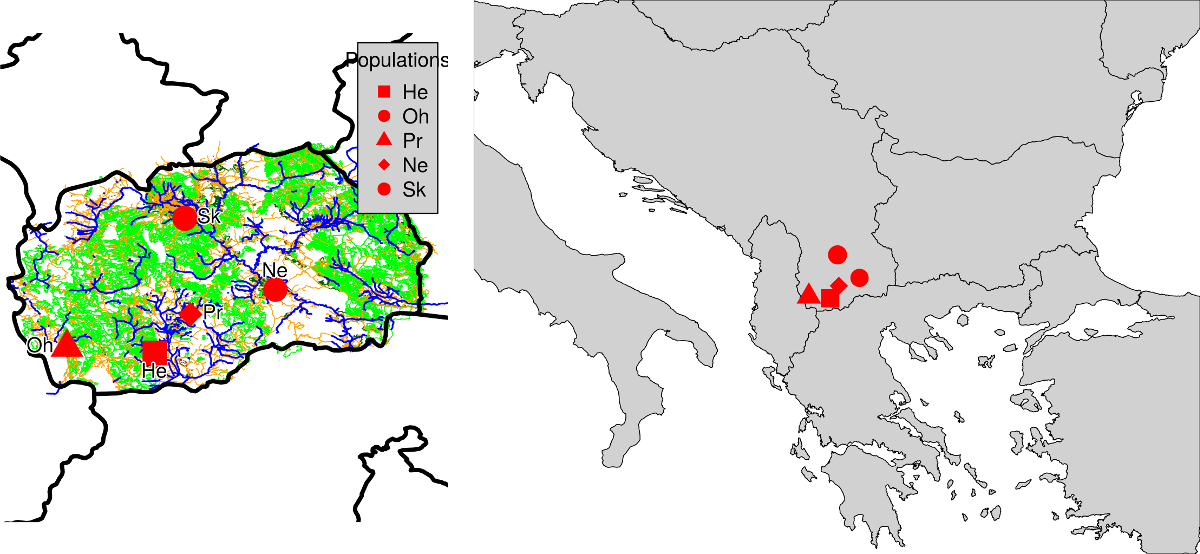
\includegraphics[width=\textwidth]{mapy.png}
  \vfil
\end{frame}

\section{Structure}

\begin{frame}{Structure}
  \begin{itemize}
    \item Population genetic software for Bayesian clustering, \url{http://pritchardlab.stanford.edu/structure.html}
    \item Uses Bayesian algorithm to find optimal distribution of individuals into the most natural number of groups (K)
    \item One Structure run tests one selected K
    \begin{itemize}
      \item User must run it repeatedly for several Ks to find the best division
      \item User must run it repeatedly for each K to see if the result is stable (because of stochasticity of the computational algorithm)
      \item Finally there use to be hundreds of runs\ldots
      \item Structure has Java GUI to set up repeated runs -- another possibility is to use R (or possibly any other scripting language like BASH, Perl or Python)
    \end{itemize}
    \item Full procedure (parallel running of Structure using R and post-processing results with R and BASH) for Linux/UNIX computers is described at \url{https://trapa.cz/en/structure-r-linux}
  \end{itemize}
\end{frame}

\begin{frame}{Structure work flow}
  \begin{enumerate}
    \item Run multiple runs of Structure
    \begin{itemize}
      \item User must test several numbers of genetic clusters (K) and test each several times
      \item ParallelStructure (see later) can do this
    \end{itemize}
    \item Decide which K is the best -- explore outputs
    \begin{itemize}
      \item Plain command line Structure does not help with this
      \item There is need for external application reading Structure output, summing them and helping decide which K is the best
      \item \href{http://taylor0.biology.ucla.edu/structureHarvester/}{Structure Harvester} or Structure-sum R script (see later) can do this
    \end{itemize}
    \item Post process Structure outputs to prepare them for plotting
    \begin{itemize}
      \item Sort and align Structure outputs
      \item Probably most commonly done in \href{https://web.stanford.edu/group/rosenberglab/clumpp.html}{CLUMPP}
    \end{itemize}
    \item Plot the final graphs
    \begin{itemize}
      \item Can be done in nearly any enough advanced graphical tool (including some R functions), probably the most commonly used is \href{https://web.stanford.edu/group/rosenberglab/distruct.html}{distruct}
    \end{itemize}
  \end{enumerate}
\end{frame}

\subsection{Running Structure from R}

\begin{frame}[fragile]{Running Structure in parallel with R}
  \begin{itemize}
    \item Let's use modern multi-core CPUs and plenty of RAM in current computers -- parallelisation saves time
    \item \href{https://r-forge.r-project.org/R/?group_id=1636}{ParallelStructure} R library can optimally distribute computations of independent Structure runs among CPU cores
    \item When using it, cite \href{http://www.plosone.org/article/info\%3Adoi\%2F10.1371\%2Fjournal.pone.0070651}{Besnier \& Glover 2013}
    \item I~show slightly modified way from \href{http://www.molecularecologist.com/2013/09/using-r-to-run-parallel-analysis-of-population-genetic-data-in-structure-parallelstructure/}{The Molecular Ecologist}
    \item Authors recommend to run it without GUI and not on Windows\ldots
    \item For this chapter start new R project in new working directory
  \end{itemize}
  \begin{spluscode}
    # Prepare special new empty directory and set working directory
    setwd("~/dokumenty/fakulta/vyuka/r_mol_data/examples/structure/")
    install.packages("ParallelStructure",
      repos="https://r-forge.r-project.org") # Install the package
    library(ParallelStructure) # Load the library
    # It takes more or less same parameter as normal Structure
    ?parallel_structure # See Structure manual and function's documentation
  \end{spluscode}
\end{frame}

\begin{frame}{Preparing for ParallelStructure}
  Within working ``structure'' directory you need
  \begin{itemize}
    \item Subdirectory for results
    \item Text file describing jobs (``joblist'')
      \begin{itemize}
	\item One row for one Structure run
	\item Every line contains name of run, list of populations separated by comas (e.g. 1,2,3,4,5) -- you don't have to use all populations in all runs
	\item K~for actual run
	\item Length of burnin chain
	\item Number of steps (in practice use much higher number than for the example -- also for length of burnin chain)
	\item Columns are separated by spaces (or TABs)
      \end{itemize}
    \item Data input file (see Structure manual)
      \begin{itemize}
	\item Make it as simple as possible -- remove all unneeded columns
	\item For population names use subsequent numbers from 1~to number of populations
	\item For individual names use only alphanumerical characters
    \end{itemize}
  \end{itemize}
\end{frame}

\begin{frame}[fragile]{Input files}
  \vfil
  \textbf{Joblist file:}
  \vfil
  \begin{tabular}{lllll}
    S02 & 1,2,3,4,5 & 1 & 500 & 10000\\
    S06 & 1,2,3,4,5 & 2 & 500 & 10000\\
    S08 & 1,2,3,4,5 & 2 & 500 & 10000\\
    ... & ... & ... & ... & ...
  \end{tabular}
  \vfill
  \textbf{Input file:}
  \vfil
  \begin{tabular}{lllllllllll}
    & & & msta93 & msta101 & msta102 & msta103 & ...\\
    H01 & 1 & 0 & 269 & 198 & 221 & 419 & ...\\
    H01 & 1 & 0 & 269 & 198 & 223 & 419 & ...\\
    H02 & 1 & 0 & 275 & 198 & 221 & 419 & ...\\
    H02 & 1 & 0 & 283 & 198 & 223 & 419 & ...\\
    ... & ... & ... & ... & ... & ... & ... & ...
  \end{tabular}
  \vfil
\end{frame}

\begin{frame}[fragile]{Running ParallelStructure}
  \begin{spluscode}
    parallel_structure(joblist="joblist.txt", n_cpu=3, structure_path=
      "~/bin/", infile="hauss_stru.in", outpath="results/", numinds=47,
      numloci=12, plot_output=1, label=1, popdata=1, popflag=1,
      phenotypes=0, markernames=1, mapdist=0, onerowperind=0, phaseinfo=0,
      extracol=0, missing=-9, ploidy=2, usepopinfo=0, revert_convert=1,
      printqhat=1, locdata=0, recessivealleles=0, phased=0, noadmix=0,
      linkage=0, locprior=0, inferalpha=1)
  \end{spluscode}
  \begin{itemize}
    \item Choose \texttt{n\_cpu} according to your computer
    \item \texttt{structure\_path} points to \alert{directory} containing Structure binary
    \item \texttt{outpath} should aim to \alert{empty} directory
    \item \texttt{plot\_output=1} will produce plots for all runs
    \item Check all other settings according to Structure manual and your needs
    \item Get toy input file \url{https://soubory.trapa.cz/rcourse/hauss_stru.in} and joblist \url{https://soubory.trapa.cz/rcourse/joblist.txt}
  \end{itemize}
\end{frame}

\subsection{ParallelStructure on Windows}

\begin{frame}[fragile]{ParallelStructure and Windows}
  \begin{itemize}
    \item Authors do not recommend to run ParallelStructure on Windows\ldots
    \item \texttt{parallel\_structure()} uses for parallelisation library which is not available on Windows, instead try
  \end{itemize}
  \begin{spluscode}
    # Install Rmpi library required by ParallelStructure for
    # parallelisation on Windows (installation can be very problematic)
    install.packages("Rmpi")
    library(Rmpi)
    # Instead of parallel_structure() use MPI_structure()
    # with same arguments
    MPI_structure(...) # Same arguments as on previous slide
  \end{spluscode}
  \begin{itemize}
    \item It may help to set \texttt{n\_cpu=1}, but it is only for testing then, not for real work...
    \item If this fails, look for some UNIX machine (Linux, Mac OS~X, BSD,~\ldots)\ldots
  \end{itemize}
\end{frame}

\subsection{Post processing}

\begin{frame}[fragile]{Post process Structure results -- select the best K}
  \begin{itemize}
    \item Using Structure-sum-2011 R script by \href{http://en.uit.no/om/enhet/ansatte/person?p_document_id=41186&p_dimension_id=88165}{Dorothee Ehrich}
  \end{itemize}
 \begin{spluscode}
    # Load the script
    source("https://soubory.trapa.cz/rcourse/structure-sum-2011.r")
    # Create new directory with result files results_job_*_f and set
    # working directory accordingly
    setwd("/home/vojta/dokumenty/fakulta/vyuka/r_mol_data/examples/
      structure/structure_sum/")
  \end{spluscode}
  \begin{itemize}
    \item When using it, cite \href{http://onlinelibrary.wiley.com/doi/10.1111/j.1471-8286.2006.01380.x/abstract}{Ehrich 2006}. If you don't have the script, ask (it is not my so I~don't want to post it on the net), see \href{https://soubory.trapa.cz/rcourse/structure-sum-2011.pdf}{manual}
    \item Prepare \textbf{list\_k.txt} containing on each line K~and name of output file
    \item Get list K~(example of the joblist below) from \url{https://soubory.trapa.cz/rcourse/list_k.txt}
  \end{itemize}
  \vfil
  \begin{tabular}{ll}
    2 & results\_job\_S010\_f\\
    3 & results\_job\_S011\_f\\
    \ldots & \ldots
  \end{tabular}
\end{frame}

\begin{frame}[fragile]{Run Structure-sum}
  \begin{spluscode}
    # See documentation for details. Functions take as an argument
    # list_k file and number of populations
    Structure.table("list_k.txt", 5)
    Structure.simil("list_k.txt", 5)
    Structure.deltaK("list_k.txt", 5)
    graphics.off() # Close graphics
    Structure.cluster("list_k.txt", 5)
    # Reordering ("alignment") of runs to get same clusters in same
    # columns (prepare respective list_k files - one for each K)
    Structure.order("list_k_02.txt", 5)
    Structure.order("list_k_03.txt", 5)
    Structure.order("list_k_04.txt", 5)
    Structure.order("list_k_05.txt", 5)
    Structure.order("list_k_06.txt", 5)
    Structure.order("list_k_07.txt", 5)
    # Continue with CLUMPP and distruct...
  \end{spluscode}
  \begin{itemize}
    \item Details: \url{https://trapa.cz/en/structure-r-linux}
  \end{itemize}
\end{frame}

\begin{frame}{Outputs of Structure-sum -- the best K~is 2, may be 3~-- stability of runs, good posterior probability}{Results from different data set, not from our toy}
  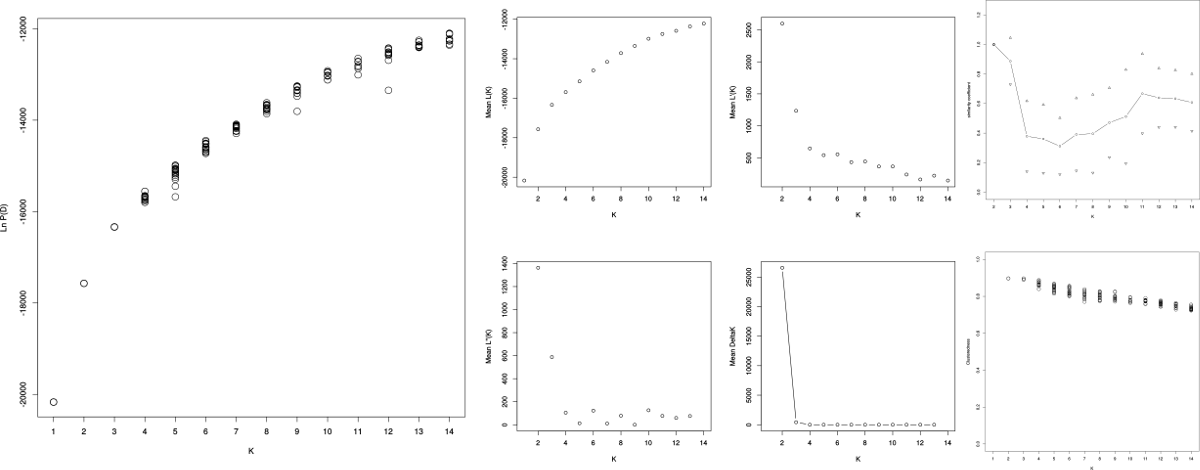
\includegraphics[width=\textwidth]{structure.png}
\end{frame}

\begin{frame}{Example of final Structure plot}{Drawn by distruct after alignment of Structure outputs by CLUMPP}
  \begin{itemize}
    \item Each bar is one individual
    \item Each color is one genetic cluster (here is shown clustering for K=12)
    \item Individuals with columns composing of more colors are genetically mixture of more clusters
    \item Details: \url{https://trapa.cz/en/structure-r-linux}
  \end{itemize}
  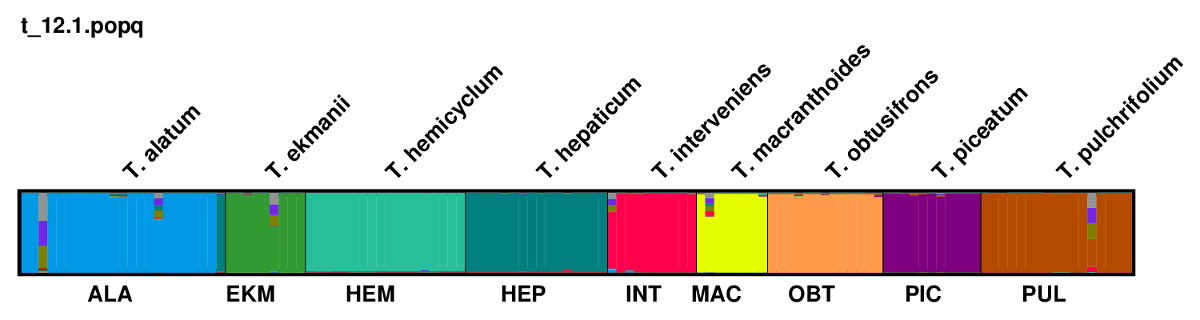
\includegraphics[width=\textwidth]{structure-fin.png}
\end{frame}

\section{Alignment}

\begin{frame}{Multiple sequence alignment}
  \begin{itemize}
    \item Good alignment is basic condition for any analysis of DNA sequences
    \item R doesn't have any possibility for visual editing (use rather software like \href{http://www.geneious.com/}{Geneious}, \href{http://www.clcbio.com/products/clc-sequence-viewer/}{CLC Sequence Viewer} or \href{http://www.mbio.ncsu.edu/bioedit/bioedit.html}{BioEdit})
    \item R can automatically (in batch) run multiple sequence alignments of multiple genes (there are several possibilities)
    \begin{itemize}
      \item Simple scripts for this task can be written in any scripting language like BASH, Perl or Python -- only matters what user likes, knows and wish to do with the results\ldots
    \end{itemize}
    \item R packages use common alignment software: \href{http://mafft.cbrc.jp/alignment/software/}{MAFFT}, \href{http://www.drive5.com/muscle/}{MUSCLE}, \href{http://www.clustal.org/}{Clustal},~\ldots
    \begin{itemize}
      \item User must install this software manually -- R is just using external applications (in the examples shown)
    \end{itemize}
  \end{itemize}
\end{frame}

\subsection{Overview and MAFFT}

\begin{frame}[fragile]{Multiple sequence alignment with MAFFT}
  \begin{itemize}
    \item MUSCLE is available in packages \texttt{muscle} and \texttt{ape} -- first one reads ``\texttt{*StringSet}'' class R objects and writes ``\texttt{*MultipleAlignment}'' R objects; the latter reads and writes object of class ``\texttt{DNAbin}''
    \item \texttt{ape} also contains functions to use Clustal and T-Coffee -- both read and write \texttt{DNAbin}
    \item MAFFT is available from (same author) in packages \href{https://cran.r-project.org/web/packages/ips/index.html}{ips} and \href{http://www.christophheibl.de/Rpackages.html}{phyloch} -- both read and write \texttt{DNAbin}
  \end{itemize}
  \begin{spluscode}
    library(colorspace) # Libraries needed by phyloch/ips
    library(XML)
    library(phyloch) # Alignment with mafft, you can also try package ips
    # Requires path to MAFFT binary - set it according to your installation
    # read ?mafft and mafft's documentation
    meles.mafft <- mafft(x=meles.dna, method="localpair", maxiterate=100,
      path="/usr/bin/mafft") # Change "path" to fit your path to mafft!
  \end{spluscode}
\end{frame}

\subsection{MAFFT, Clustal, MUSCLE and T-Coffee}

\begin{frame}[fragile]{Clustal, MUSCLE and T-Coffee from ape}
  \begin{spluscode}
    meles.mafft
    class(meles.mafft)
    # read ?clustal and documentation of Clustal, Muscle and T-Coffee
    # when using them to set correct parameters
    meles.clustal <- ape::clustal(x=meles.dna, pw.gapopen=10, pw.gapext=0.1,
      gapopen=10, gapext=0.2, exec="/usr/bin/clustalw2", quiet=FALSE,
      original.ordering=TRUE) # Change "exec" to fit your path to clustal!
    meles.muscle <- muscle(x=meles.dna, exec="muscle", quiet=FALSE,
      original.ordering=TRUE) # Change "exec" to fit your path to muscle!
    meles.muscle
    class(meles.muscle)
    # Plot the alignment - you can select which bases to plot
    # and/or modify colors
    image(x=meles.muscle, c("a", "t", "c" ,"g", "n"), col=rainbow(5))
    # Add grey dotted grid
    grid(nx=ncol(meles.muscle), ny=nrow(meles.muscle), col="lightgrey")
    # Remove gaps from alignment - destroy it
    meles.nogaps <- del.gaps(meles.muscle) # See ?del.gaps for details!
  \end{spluscode}
\end{frame}

\subsection{Display and cleaning}

\begin{frame}{Multiple sequence alignment with MUSCLE}
  \includegraphics[width=\textwidth]{muscle.png}
\end{frame}

\begin{frame}[fragile]{Cleaning the alignment}
  \begin{spluscode}
    # Shortcut for plotting alignment
    image.DNAbin(x=meles.mafft)
    # Display aligned sequences with gaps
    image.DNAbin(x=usflu.dna)
    # Delete all columns containing any gap
    library(ips)
    usflu.dna.ng <- deleteGaps(x=usflu.dna, nmax=0)
    # See of settings of "nmax" value - threshold for gap deletion
    ?deleteGaps # "nmax=0" deletes all columns with any gap
    # Do not confuse with function delete.gaps() from phyloch package
    # Display the result
    image.DNAbin(x=usflu.dna.ng)
    # Delete positions in alignment containing only missing data/N
    ?deleteEmptyCells # See help page for details
  \end{spluscode}
\end{frame}

\section{Trees}

\subsection{Manipulations}

\begin{frame}[fragile]{Read and write tree and drop tips}
  \begin{spluscode}
    # Read trees in NEWICK format - single or multiple tree(s)
    oxalis.trees <- read.tree
      ("https://soubory.trapa.cz/rcourse/oxalis.nwk")
    summary(oxalis.trees)
    length(oxalis.trees)
    names(oxalis.trees)
    # Export trees in NEWICK format
    write.tree(phy=oxalis.trees, file="trees.nwk")
    # Drop a tip from multiPhylo
    plot.multiPhylo(x=oxalis.trees)
    oxalis.trees.drop <- lapply(X=oxalis.trees, FUN=drop.tip, "TaxaOut")
    class(oxalis.trees.drop) <- "multiPhylo"
    plot.multiPhylo(x=oxalis.trees.drop)
    # Drop a tip from single tree
    plot.phylo(hauss.nj)
    hauss.nj.drop <- drop.tip(phy=hauss.nj, tip=47)
    plot.phylo(hauss.nj.drop)
  \end{spluscode}
\end{frame}

\begin{frame}[fragile]{Extract clades from trees and drop extinct tips}
  \begin{spluscode}
    # Interactively extract tree
    # Plot source tree
    plot.phylo(hauss.nj)
    nodelabels() # See node labels (numbers) - needed for some tasks
    # Select clade to extract by clicking on it
    hauss.nj.extracted <- extract.clade(phy=hauss.nj, interactive=TRUE)
    # See new extracted tree
    plot.phylo(hauss.nj.extracted)
    # Non-interactively extract tree
    hauss.nj.extracted <- extract.clade(phy=hauss.nj, node=60,
      interactive=FALSE)
    # See new extracted tree
    plot.phylo(hauss.nj.extracted)
    # Drop "extinct" tips - those who don't reach end the tree
    # tolerance is respective to the used metrics
    plot.phylo(hauss.nj)
    axisPhylo()
    hauss.nj.fossil <- drop.fossil(phy=hauss.nj, tol=0.4)
    plot.phylo(hauss.nj.fossil)
  \end{spluscode}
\end{frame}

\begin{frame}[fragile]{Join two trees, rotate tree}
  \begin{spluscode}
    # Bind two trees into one
    hauss.nj.bind <- bind.tree(x=hauss.nj.fossil, y=hauss.nj.extracted,
      where="root", position=0, interactive=FALSE)
    plot.phylo(hauss.nj.bind)
    # Bind two trees interactively
    # Plot tree receiving the new one
    plot.phylo(hauss.nj.fossil)
    # Select where to bind new tree to
    hauss.nj.bind <- bind.tree(x=hauss.nj.fossil, y=hauss.nj.extracted,
      interactive=TRUE)
    plot.phylo(hauss.nj.bind)
    # Rotate tree
    plot.phylo(hauss.nj)
    nodelabels()
    hauss.nj.rotated <- rotate(phy=hauss.nj, node="70")
    plot.phylo(hauss.nj.rotated)
  \end{spluscode}
\end{frame}

\begin{frame}[fragile]{Ladderize and (un)root the tree}
  \begin{spluscode}
    # Ladderize the tree
    plot.phylo(hauss.nj)
    hauss.nj.ladderized <- ladderize(hauss.nj)
    plot.phylo(hauss.nj.ladderized)
    # Root the tree
    plot.phylo(hauss.nj)
    print.phylo(hauss.nj)
    # resolve.root=TRUE ensures root will be bifurcating (needed here)
    # (without this parameter it soemtimes doesn't work)
    hauss.nj.rooted <- root(phy=hauss.nj, resolve.root=TRUE, outgroup=10)
    print.phylo(hauss.nj.rooted)
    plot.phylo(hauss.nj.rooted)
    # Root the tree interactive
    plot.phylo(hauss.nj)
    hauss.nj.rooted <- root(phy=hauss.nj, interactive=TRUE)
    plot.phylo(hauss.nj.rooted)
    unroot() # unroot the tree
    # Check if it is rooted is.rooted()
  \end{spluscode}
\end{frame}

\begin{frame}[fragile]{Check tree and compute branch lengths and times}
  \begin{spluscode}
    # Check if the tree is ultrametric - is variance of distances
    # of all tips to node 0? It is required for some analysis
    is.ultrametric()
    # Make tree ultrametric
    chronos()
    ?chronos # Check it for mode how to calculate the lengths
    # chronos has more uses - it is mainly used for dating
    # Compute branch lengths for trees without branch lengths
    ?compute.brlen # Check it for mode how to calculate the lengths
    compute.brlen()
    # Computes the branch lengths of a tree giving its branching
    # times (aka node ages or heights)
    compute.brtime()
    ?compute.brtima # Check it for mode how to calculate the lengths
  \end{spluscode}
  \begin{itemize}
    \item Class \texttt{multiPhylo} is just a~\texttt{list} of \texttt{phylo} objects to store multiple trees -- you can perform most of analysis on it as on \texttt{phylo}, commonly using \texttt{lapply} function (afterward use \texttt{class(x) <- "multiPhylo"} to ensure other functions will see it as \texttt{multiPhylo} object)
  \end{itemize}
\end{frame}

\subsection{Seeing trees in the forest}

\begin{frame}{Topographical distances among matrices I -- implementations}
  \begin{itemize}
    \item Robinsons-Foulds distance in \texttt{phytools::multiRF}
    \begin{itemize}
      \item The index adds 1 for each difference between pair of trees
      \item Well defined only for fully bifurcating trees -- if not fulfilled, some results might be misleading
      \item Allow comparison of trees created by different methods
    \end{itemize}
    \item Methods implemented in \texttt{ape::dist.topo} allow comparison of trees with polytomies (\texttt{method="PH85"}) or use of squared lengths of internal branches (\texttt{method="score"})
    \item Final matrices are commonly not \href{https://en.wikipedia.org/wiki/Euclidean_distance_matrix}{Euclidean} -- may be problematic for usage in methods like PCA
    \begin{itemize}
      \item Test it with \texttt{ade4::is.euclid}, can be scaled (forced to became Euclidean) by functions like \texttt{quasieuclid} or \texttt{cailliez} in \texttt{ade4} -- carefully, it can damage meaning of the data
    \end{itemize}
  \end{itemize}
\end{frame}

\begin{frame}[fragile]{Topographical distances among trees II}{We have plenty of trees. How much are their topologies different?}
  \begin{spluscode}
    library(gplots)
    library(corrplot)
    library(phytools)
    # Prepare matrix for distances
    oxalis.trees.d <- matrix(nrow=length(oxalis.trees),
      ncol=length(oxalis.trees))
    # Calculate pairwise topographic distances
    for (i in 1:length(oxalis.trees)) {
      for (j in i:length(oxalis.trees)) {
        print(c(i,j))
        oxalis.trees.d[i,j] <- dist.topo(oxalis.trees[[i]],
          oxalis.trees[[j]])
      }
    } # dist.topo can compare only two trees in one step... :-(
    # Basic information about the distance matrix
    dim(oxalis.trees.d)
    head.matrix(oxalis.trees.d)
  \end{spluscode}
\end{frame}

\begin{frame}[fragile]{Topographical distances among trees III}{Post process the matrix and plot it}
  \begin{itemize}
    \item There are several methods for calculating distance matrices among the trees -- some take branch lengths into account, some only topology
  \end{itemize}
  \begin{spluscode}
    colnames(oxalis.trees.d) <- names(oxalis.trees) # Add names of
    rownames(oxalis.trees.d) <- names(oxalis.trees) # columns and rows
    # Make matrix symmetric
    oxalis.trees.d[lower.tri(oxalis.trees.d)] <-
      t(oxalis.trees.d)[lower.tri(oxalis.trees.d)]
    # Create heatmaps using heatmap.2 function from gplots package
    heatmap.2(x=oxalis.trees.d, Rowv=FALSE, Colv="Rowv", dendrogram="none",
      symm=TRUE, scale="none", na.rm=TRUE, revC=FALSE, col=rainbow(15),
      cellnote=oxalis.trees.d, notecex=1, notecol="white", trace="row",
      linecol="black", labRow=names(oxalis.trees),
      labCol=names(oxalis.trees), key=TRUE, keysize=2,
      density.info="density", symkey=FALSE, main="Correlation matrix of
      topographical distances", xlab=names(oxalis.trees),
      ylab=names(oxalis.trees))
  \end{spluscode}
\end{frame}

\begin{frame}[fragile]{Topographical distances among trees IV}{Calculate Robinsons-Foulds distance matrix among trees and plot it}
  \begin{itemize}
    \item \texttt{phytools::multiRF} can handle \texttt{multiPhylo} objects and directly create matrices (no need to create loops)
  \end{itemize}
  \begin{spluscode}
    # Robinsons-Foulds distance
    oxalis.trees.d.rf <- multiRF(oxalis.trees)
    # Add names of columns and rows
    colnames(oxalis.trees.d.rf) <- names(oxalis.trees)
    rownames(oxalis.trees.d.rf) <- names(oxalis.trees)
    # Create heatmap using corrplot function from corrplot package
    corrplot(corr=oxalis.trees.d.rf, method="circle", type="upper",
      col=rainbow(15), title="Correlation matrix of topographical
      distances", is.corr=FALSE, diag=FALSE, outline=TRUE,
      order="alphabet", tl.pos="lt", tl.col="black")
    corrplot(corr=oxalis.trees.d.rf, method="number", type="lower",
      add=TRUE, col=rainbow(15), title="Correlation matrix of
      topographical distances", is.corr=FALSE, diag=FALSE,
      outline=FALSE, order="alphabet", tl.pos="ld", cl.pos="n")
  \end{spluscode}
\end{frame}

\begin{frame}{Topographical distances among trees V -- the matrices}
  \includegraphics[width=\textwidth]{oxalis-dist.png}
\end{frame}

\begin{frame}[fragile]{PCoA from distance matrices of topographical differences among trees -- the code}{PC plots help to identify outliers -- trees with noticeably different topology}
  \begin{spluscode}
    # Test if the distance matrix is Euclidean or not
    is.euclid(distmat=as.dist(oxalis.trees.d), plot=TRUE)
    [1] TRUE # OK. If it wouldn't be, we could use e.g. quasieuclid()
    # Calculate the PCoA
    oxalis.trees.pcoa <- dudi.pco(d=as.dist(oxalis.trees.d), scannf=TRUE,
      full=TRUE)
    # Plot PCoA
    s.label(dfxy=oxalis.trees.pcoa$li)
    # Add kernel densities
    s.kde2d(dfxy=oxalis.trees.pcoa$li, cpoint=0, add.plot=TRUE)
    # Add histogram of eigenvalues
    add.scatter.eig(oxalis.trees.pcoa[["eig"]], 3,1,2, posi="topleft")
    # Add title to the plot
    title("\nPCoA of matrix of pairwise trees distances")
    # Alternative function to plot PCA plot
    scatter(x=oxalis.trees.pcoa, posieig="topleft")
  \end{spluscode}
\end{frame}

\begin{frame}{PCoA from distance matrices of topographical differences among trees -- the plot}
  \begin{center}
    \includegraphics[height=6cm]{pcoa-trees.png}
  \end{center}
\end{frame}

\begin{frame}[fragile]{Consensus tree}
\begin{multicols}{2}
  \includegraphics[height=6cm]{oxalis-cons.png}
  \begin{spluscode}
    # Root all trees
    oxalis.trees.rooted <- lapply
      (X=oxalis.trees, FUN=root,
      "TaxaOut")
    class(oxalis.trees.rooted) <-
      "multiPhylo"
    # Consensus tree (50 % rule)
    oxalis.tree.con <- consensus
      (oxalis.trees.rooted, p=0.5,
      check.labels=TRUE)
    print.phylo(oxalis.tree.con)
    # Plot the tree
    plot.phylo(oxalis.tree.con,
      edge.width=2, label.offset=0.3)
    axisPhylo(side=1)
    # What a nice tree... :-P
  \end{spluscode}
\end{multicols}
\end{frame}

\begin{frame}[fragile]{Species tree -- all trees must be ultrametric}
\begin{multicols}{2}
\includegraphics[height=6cm]{oxalis-sp.png}
  \columnbreak
  \begin{spluscode}
    # Chronos scale trees
    oxalis.trees.ultra <- lapply
      (X=oxalis.trees.rooted,
      FUN=chronos, model="correlated")
    class(oxalis.trees.ultra) <-
      "multiPhylo"
    # Mean distances
    oxalis.tree.sp.mean <- speciesTree
      (oxalis.trees.ultra, mean)
    # Plot the tree
    plot.phylo(oxalis.tree.sp.mean,
      edge.width=2, label.offset=0.01)
    edgelabels(text=round(oxalis.
      tree.sp.mean[["edge.length"]],
      digits=2), frame="none",
      col="red", bg="none")
    axisPhylo(side=1)
  \end{spluscode}
\end{multicols}
\end{frame}

\begin{frame}[fragile]{Parsimony super tree}
\begin{multicols}{2}
  \includegraphics[height=6cm]{oxalis-pars.png}
  \begin{spluscode}
    library(phangorn)
    oxalis.tree.sp <- superTree(tree=
      oxalis.trees.rooted, method=
      "optim.parsimony", rooted=TRUE)
    print.phylo(oxalis.tree.sp)
    plot.phylo(oxalis.tree.sp,
      edge.width=2, label.offset=0.01)
    axisPhylo(side=1)
  \end{spluscode}
\end{multicols}
\end{frame}

\begin{frame}[fragile]{Density tree}
  \begin{spluscode}
    densiTree(x=oxalis.trees.ultra, type="cladogram", alpha=0.5,
      consensus=oxalis.tree.sp.mean, scaleX=TRUE, col=c("black",
      "green", "blue", "red"), cex=1.5)
  \end{spluscode}
  \begin{center}
    \includegraphics[width=\textwidth-1.5cm]{oxalis_density_good.png}
  \end{center}
\end{frame}

\begin{frame}[fragile]{Networks}
\begin{multicols}{2}
  \vfil
  \begin{spluscode}
    oxalis.tree.net <- consensusNet
      (oxalis.trees.rooted, prob=0.25)
  \end{spluscode}
  \vfil
  \includegraphics[height=5.5cm]{oxalis-net.png}
  \vfil
  \begin{spluscode}
    plot.networx(x=oxalis.tree.net,
      planar=FALSE, type="2D",
      use.edge.length=TRUE,
      show.tip.label=TRUE,
      show.edge.label=TRUE,
      show.node.label=TRUE,
      show.nodes=TRUE,
      edge.color="black",
      tip.color="blue") # 2D - left
    plot.networx(x=oxalis.tree.net,
      planar=FALSE, type="3D",
      use.edge.length=TRUE,
      show.tip.label=TRUE,
      show.edge.label=TRUE,
      show.node.label=TRUE,
      show.nodes=TRUE, edge.color=
      "black", tip.color="blue") # 3D
  \end{spluscode}
\end{multicols}
\end{frame}

\begin{frame}[fragile]{Kronoviz -- see all trees on same scale}
\begin{multicols}{2}
  \includegraphics[height=5.5cm]{kronoviz.png}
  \begin{spluscode}
    kronoviz(x=oxalis.trees.rooted,
      layout=length(oxalis.trees.
      rooted), horiz=TRUE)
    # Close graphical device to
    # cancel division of plotting
    # device
    dev.off()
  \end{spluscode}
  \vfill
  \begin{itemize}
    \item The plot can be very long and it can be hard to see details
    \item But one can get impression if all trees are more or less in same scale (have comparable length) or not
  \end{itemize}
  \vfil
\end{multicols}
\end{frame}

\subsection{MP}

\begin{frame}{Maximum parsimony -- theory}
  \label{MP}
  \begin{itemize}
    \item \href{https://en.wikipedia.org/wiki/Maximum_parsimony_(phylogenetics)}{Maximum parsimony} finds optimal topology of the phylogenetic tree by minimizing of the total number of character-state changes
    \item It minimizes homoplasy (convergent evolution, parallel evolution, evolutionary reversals)
    \item Very simple criterion, easy to score the tree, but not to find it -- exhaustive search to explore all possible trees is realistic until $\sim$9 taxa, branch-and-bound swapping (guaranteeing finding the best tree) until $\sim$20 taxa, for more heuristic search is needed -- it doesn't always guarantee to find the most probable tree
    \item To speed up calculations, initial tree (usually NJ -- slide~\ref{NJ}) is used to start the search
    \item With rising performance of computers, it use to replaced my maximum likelihood or Bayesian methods
  \end{itemize}
\end{frame}

\begin{frame}[fragile]{Maximum parsimony -- code and result}
\begin{multicols}{2}
  \vfil
  \includegraphics[height=6cm]{parsimony.png}
  \vfil
  \splus/?parsimony # Parsimony details/
  \vfil
  \begin{spluscode}
    # Conversion to phyDat
    meles.phydat <-
      as.phyDat(meles.dna)
    # Prepare starting tree
    meles.tre.ini <- nj(dist.
      dna(x=meles.dna,model="raw"))
    # Maximum parsimony score
    parsimony(tree=meles.tre.ini,
      data=meles.phydat)
    # Optimization
    # Maximum parsimony tree
    meles.tre.pars <- optim.
      parsimony(tree=meles.tre.
      ini, data=meles.phydat)
    # Draw a tree
    plot.phylo(x=meles.tre.pars,
      type="clad", edge.width=2)
  \end{spluscode}
\end{multicols}
\end{frame}

\subsection{Comparisons}

\begin{frame}[fragile]{Compare two trees}
  \begin{spluscode}
    # Compare topology of the species trees - basically outputs TRUE/FALSE
    all.equal.phylo(oxalis.tree.sp, oxalis.tree.sp.mean,
      use.edge.length=FALSE)
    ?all.equal.phylo # Use to see comparison possibilities
    # Plot two trees with connecting lines
    # We need 2 column matrix with tip labels
    tips.labels <- matrix(data=c(sort(oxalis.tree.sp[["tip.label"]]),
      sort(oxalis.tree.sp.mean[["tip.label"]])),
      nrow=length(oxalis.tree.sp[["tip.label"]]), ncol=2)
    # Draw a tree - play with graphical parameters and use rotate=TRUE
    # to be able to adjust fit manually
    cophyloplot(x=ladderize(oxalis.tree.sp),
      y=ladderize(oxalis.tree.sp.mean),  assoc=tips.labels,
      use.edge.length=FALSE, space=60, length.line=1, gap=2,
      type="phylogram", rotate=TRUE, col="red", lwd=1.5, lty=2)
    title("Comparing the trees\nParsimony super tree\tSpecies tree")
    legend("topleft", legend="Red lines\nconnect tips", text.col="red",
      cex=0.75, bty="n", x.intersp=-2, y.intersp=-2)
  \end{spluscode}
\end{frame}

\begin{frame}{Cophyloplot comparing two trees}
  \begin{multicols}{2}
    \includegraphics[height=6cm]{cophyloplot.png}
    \begin{itemize}
      \item \texttt{ladderize()} pre-sorts tips in the tree -- it helps to \texttt{cophyloplot()} to create better plot
      \item Automatic plot is usually not perfect -- there use to be unneeded crossing lines -- \texttt{rotate=TRUE} is recommended to can fix this manually by clicking to the nodes
      \item \texttt{cophyloplot()} has similar parameters like \texttt{plot.phylo()} -- play with it and adjust in graphical editor
    \end{itemize}
  \end{multicols}
\end{frame}

\subsection{Notes about plotting the trees}

\begin{frame}[fragile]{Change orientation of plots}
  \begin{itemize}
    \item \alert{\texttt{plot.phylo()} has plenty of possibilities to influence -- check \texttt{?plot.phylo}, \texttt{?par}, \texttt{?points},~\ldots}
  \end{itemize}
  \begin{spluscode}
    ?plot.phylo # check it for various possibilities what to influence
    par(mfrow=c(1, 2)) # Plot two plots in one row
    plot.phylo(x=hauss.nj, type="cladogram", use.edge.length=FALSE,
      direction="rightwards")
    plot.phylo(x=hauss.nj, type="cladogram", use.edge.length=FALSE,
      direction="leftwards")
    dev.off() # Close graphical device to cancel par() settings
  \end{spluscode}
  \begin{center}
    \includegraphics[height=3cm]{lr.png}
  \end{center}
\end{frame}

\begin{frame}[fragile]{Highlighted labels}
\begin{multicols}{2}
  \vfill
  \includegraphics[height=5cm]{highlight.png}
  \vfill
  \begin{spluscode}
    # Load tree in text format
    trape <- read.tree(text=
      "((Homo, Pan), Gorilla);")
    # Plot the tree
    plot.phylo(x=trape,
      show.tip.label=FALSE)
    # Add colored tip labels
    tiplabels(trape[["tip.label"]],
      bg=c("white", "black",
      "white"), col=c("black",
      "white", "black"), cex=2)
    # Add colored node labels
    nodelabels(text=c("6.4 Ma",
      "5.4 Ma"), frame="circle",
      bg="yellow")
    add.scale.bar() # Add scale bar
    # Note vectors for tip/nodelabels
  \end{spluscode}
\end{multicols}
\end{frame}

\section{Evolution}

% \begin[allowframebreaks]{frame}{} % TODO Introduction to methods
%   \begin{itemize}
%     \item 
%   \end{itemize}
% \end{frame}

\subsection{PIC}

\begin{frame}[fragile]{Phylogenetic independent contrast}
\begin{itemize}
 \item When analyzing comparative data takes phylogeny into account
 \item If we assume that a~continuous trait evolves randomly in any direction (i.e. the Brownian motion model), then the ``contrast'' between two species is expected to have a~normal distribution with mean zero, and variance proportional to the time since divergence
\end{itemize}
  \begin{spluscode}
    # Prepare the data # Body mass of primates
    primates.body <- c(4.09434, 3.61092, 2.37024, 2.02815, 1.46968)
    # Longevity of primates
    primates.longevity <- c(4.74493, 3.3322, 3.3673, 2.89037, 2.30259)
    # Add names to the values
    names(primates.body) <- names(primates.longevity) <- c("Homo", "Pongo",
      "Macaca", "Ateles", "Galago")
    # Create a tree in Newick format
    primates.tree <- read.tree(text="((((Homo:0.21, Pongo:0.21):0.28,
      Macaca:0.49):0.13, Ateles:0.62):0.38, Galago:1.00);")
    plot.phylo(primates.tree)
  \end{spluscode}
\end{frame}

\begin{frame}[fragile]{PIC and its plotting}
  \begin{spluscode}
    primates.pic.body <- pic(x=primates.body, phy=primates.tree,
      scaled=TRUE, var.contrasts=FALSE, rescaled.tree=FALSE)
    primates.pic.longevity <- pic(x=primates.longevity, phy=primates.tree,
      scaled=TRUE, var.contrasts=FALSE, rescaled.tree=FALSE)
    # Plot a tree with PIC values
    plot.phylo(x=primates.tree, lwd=2, cex=1.5)
    nodelabels(round(primates.pic.body, digits=3), adj=c(0, -0.5),
      frame="none")
    nodelabels(round(primates.pic.longevity, digits=3), adj=c(0, 1),
      frame="none")
    add.scale.bar()
    # Plot PIC
    plot(x=primates.pic.body, y=primates.pic.longevity, pch=16, cex=1.5)
    abline(a=0, b=1, lty=2) # x=y line
    # correlation coefficient of both PICs
    cor(x=primates.pic.body, y=primates.pic.longevity, method="pearson")
    [1] -0.5179156
  \end{spluscode}
\end{frame}

\begin{frame}{Plot of PIC (on the tree)}
  \includegraphics[width=\textwidth]{pic.png}
\end{frame}

\begin{frame}[fragile]{Test it}
  \begin{spluscode}
    lm(formula=primates.pic.longevity~primates.pic.body)
    Coefficients:
      (Intercept)  primates.pic.body
           1.6957            -0.3081
    # Because PICs have expected mean zero - such linear regressions
    # should be done through the origin (the intercept is set to zero)
    lm(formula=primates.pic.longevity~primates.pic.body-1)
    Coefficients:
    primates.pic.body
               0.4319
    # Permutation procedure to test PIC
    lmorigin(formula=primates.pic.longevity~primates.pic.body, nperm=1000)
    Regression through the origin
    Permutation method = raw data
    Coefficients and parametric test results
                       Coefficient Std_error t-value Pr(>|t|)
    primates.pic.body     0.43193   0.28649  1.5077   0.2288
    F-statistic: 2.273067 on 1 and 3 DF:
      permutational p-value: 0.2377622
  \end{spluscode}
\end{frame}

\begin{frame}[fragile]{Intraspecific variation}
  \begin{itemize}
    \item \texttt{pic.ortho()} requires list of measurements (vectors) for all taxa -- their lengths can differ
    \item If we have sets of measurements in separated vectors (each vector has measurements for all taxa), we must for each \texttt{list} item use \texttt{cbind} to join columns and select appropriate line (from 1 to number of taxa)
    \item In example below, \texttt{jitter()} adds random noise
    \item Other usage is same in previous case\ldots
  \end{itemize}
  \begin{spluscode}
    primates.pic.ortho <- pic.ortho(x=list(cbind(primates.body,
      jitter(primates.body), jitter(primates.body))[1,],cbind(primates.
      body, jitter(primates.body), jitter(primates.body))[2,],
      cbind(primates.body, jitter(primates.body), jitter(primates.body))
      [3,], cbind(primates.body, jitter(primates.body), jitter(primates.
      body))[4,], cbind(primates.body, jitter(primates.body), 
      jitter(primates.body))[5,]), phy=primates.tree, var.contrasts=FALSE,
      intra=FALSE)
  \end{spluscode}
\end{frame}

\begin{frame}[fragile]{Explanation of the cbind trick}
  \begin{spluscode}
    cbind(primates.body, jitter(primates.body), jitter(primates.body))
    Homo         4.09434 4.113074 4.038092
    Pongo        3.61092 3.671217 3.558953
    Macaca       2.37024 2.426757 2.430310
    Ateles       2.02815 1.986006 2.091402
    Galago       1.46968 1.494281 1.496831
    cbind(primates.body, jitter(primates.body), jitter(primates.body))[1,]
      4.094340      4.072501      4.035324 
    cbind(primates.body, jitter(primates.body), jitter(primates.body))[2,]
      3.610920      3.572728      3.664654 
    class(cbind(primates.body, jitter(primates.body),
      jitter(primates.body)))
    [1] "matrix"
    class(cbind(primates.body, jitter(primates.body),
      jitter(primates.body))[1,])
    [1] "numeric"
    # jitter() adds random noise every time, so that the values differ
  \end{spluscode}
\end{frame}

\subsection{Autocorrelation}

\begin{frame}[fragile]{Phylogenetic autocorrelation}
  \begin{itemize}
    \item Autocorrelation coefficient to quantify whether the distribution of a~trait among a~set of species is affected or not by their phylogenetic relationships
    \item In the absence of phylogenetic autocorrelation, the mean expected value of I~and its variance are known - it is thus possible to test the null hypothesis of the absence of dependence among observations
  \end{itemize}
  \begin{spluscode}
    # Let's choose weights as wij = 1/dij, where the d’s is the distances
    # measured on the tree - cophenetic() calculates cophenetic distances
    # can be just cophenetic(primates.tree) or some other transformation
    primates.weights <- 1/cophenetic(primates.tree)
    primates.weights # See it
    class(primates.weights)
    diag(primates.weights) <- 0 # Set diagonal to 0
\end{spluscode}
\end{frame}

\begin{frame}[fragile]{Testing of Moran's~\textit{I}}
  \begin{spluscode}
    # Calculate Moran's I
    # Slightly significant positive phylogenetic correlation among body mass
    Moran.I(x=primates.body, weight=primates.weights,
      alternative="greater")
    # Positive, but non-significant
    Moran.I(x=primates.longevity, weight=primates.weights,
      alternative="greater")
    # Test of Moran's with randomization procedure
    # Body is significant - nonrandom, longevity not (random)
    gearymoran(bilis=primates.weights, X=data.frame(primates.body,
      primates.longevity), nrepet=1000)
    # Test of Abouheif designed to detect phylogenetic autocorrelation in
    # a quantitative trait - in fact Moran's I test using a particular
    # phylogenetic proximity between tips
    library(adephylo)
    abouheif.moran(x=cbind(primates.body, primates.longevity),
      W=primates.weights, method="oriAbouheif", nrepet=1000,
      alter="greater")
  \end{spluscode}
\end{frame}

\begin{frame}[fragile]{Correlogram to visualize results of phylogenetic autocorrelation analysis}
  \begin{spluscode}
    data(carnivora) # Loads training data set
    head(carnivora) # Look at the data
    # Calculate the correlogram
    carnivora.correlogram <- correlogram.formula
      (formula=SW~Order/SuperFamily/Family/Genus, data=carnivora)
    carnivora.correlogram # See results
    # Calculate the correlogram - test for both body masses
    carnivora.correlogram2 <- correlogram.formula
      (formula=SW+FW~Order/SuperFamily/Family/Genus, data=carnivora)
    carnivora.correlogram2 # See results
    plot.correlogram(x=carnivora.correlogram, legend=TRUE,
      test.level=0.05, col=c("white", "black")) # Plot it
    # Plot it - test for both body masses - two or one graph(s)
    plot.correlogramList(x=carnivora.correlogram2, lattice=TRUE,
      legend=TRUE, test.level=0.05)
    plot.correlogramList(x=carnivora.correlogram2, lattice=FALSE,
      legend=TRUE, test.level=0.05)
  \end{spluscode}
\end{frame}

\begin{frame}{Correlograms of SW and SW+FW (in one or two graphs) depending on taxonomical level with marked significance}
  \includegraphics[width=\textwidth]{correlog.png}
\end{frame}

\subsection{Decomposition}

\begin{frame}[fragile]{Prepare toy data set (tree)}
  \begin{spluscode}
    # Load MrBayes tree in NEXUS format
    apiaceae.tree <- read.nexus
      ("https://soubory.trapa.cz/rcourse/apiaceae_mrbayes.nexus")
    print.phylo(apiaceae.tree) # See it
    plot.phylo(apiaceae.tree) # See it
    # Root the tree
    apiaceae.tree <- root(apiaceae.tree, "Aralia_elata")
    # Remove "_" from taxa names
    # plot.phylo() by default omits "_" from tip names
    apiaceae.tree$tip.label <- gsub(pattern="_", replacement=" ",
      x=apiaceae.tree$tip.label)
    # Drop outgroup (Aralia and Hydrocotyle)
    # Click on last common ancestor of ingroup desired to be kept
    plot.phylo(apiaceae.tree)
    apiaceae.tree <- extract.clade(apiaceae.tree, interactive=TRUE)
    plot.phylo(apiaceae.tree)
    library(adephylo)
    library(phylobase)
  \end{spluscode}
\end{frame}

\begin{frame}[fragile]{Modified tree}
  \vfil
  \begin{center}
    \includegraphics[width=\textwidth-0.5cm]{apiaceae_tree.png}
  \end{center}
  \vfill
  \begin{spluscode}
    # Decomposition of topographical distances (right plot)
    table.phylo4d(x=phylo4d(x=apiaceae.tree, tip.data=treePart
      (x=apiaceae.tree, result="orthobasis")), treetype="cladogram")
  \end{spluscode}
  \vfill
\end{frame}

\begin{frame}[fragile]{Prepare toy data set (the variable)}
  \begin{spluscode}
    # Generate some random variable
    library(geiger)
    apiaceae.eco <- sim.char(phy=apiaceae.tree, par=0.1, nsim=1,
      model="BM")[,,1]
    ?sim.char # See it for another possibilities to simulate data
    # Names for the values
    names(apiaceae.eco) <- apiaceae.tree[["tip.label"]]
    apiaceae.eco # See it
  \end{spluscode}
  \begin{itemize}
    \item \texttt{sim.char()} creates an array (we keep only numeric vector of 1$^{st}$ simulation -- \texttt{[,,1]}) of simulated characters, with \texttt{model="BM"} under Brownian motion
    \item Many methods compare \textbf{names} of character values with \texttt{tip.label} slot of the tree to pair character values with correct taxa
    \begin{itemize}
      \item Otherwise values must be ordered in same way as in \texttt{tip.label} slot
      \item \alert{Always check manual for respective function and all data!}
    \end{itemize}
  \end{itemize}
\end{frame}

\begin{frame}[fragile]{Orthonormal decomposition - phylogenetic eigenvector regression}
  \begin{spluscode}
    anova(lm(apiaceae.eco ~ as.matrix(orthobasis.phylo(x=apiaceae.tree,
      method="patristic")[,1:2])))
  \end{spluscode}
  \begin{itemize}
    \item Significant result -- significant phylogenetic inertia (phylogenetic effect) -- the tendency for traits to resist evolutionary change despite environmental perturbations
    \item \texttt{orthobasis.phylo()} return matrix, which is linear transformation of cophenetic distances -- columns 1 and 2 can be used to calculate phylogenetic variance -- it can be used to calculate linear regression
  \end{itemize}
  \begin{spluscode}
                 Df   Sum Sq  Mean Sq F value Pr(>F)
    as.matrix...  2 0.063689 0.031845  2.2275 0.1422
    Residuals    15 0.214443 0.014296
  \end{spluscode}
\end{frame}

\begin{frame}[fragile]{Orthonormal decomposition of variance of a quantitative variable on an orthonormal basis}
  \begin{spluscode}
    orthogram(x=apiaceae.eco, tre=apiaceae.tree, nrepet=1000,
      alter="two-sided")
    ?orthogram # See another calculation possibilities
  \end{spluscode}
  \begin{itemize}
    \item Analyses one quantitative trait
    \item Do not confuse with \texttt{ade4::orthogram} -- similar, but require data in little bit different form, marked as deprecated and replaced by the \texttt{adephylo} version
    \item It returns results of 5 non-parametric tests associated to the variance decomposition
    \item Procedure decomposes data matrix to separate phylogeny and phenotype to see if there is significant signal
  \end{itemize}
\end{frame}

\begin{frame}{Orthogram}
  \includegraphics[width=\textwidth]{orthogram.png}
  \begin{itemize}
    \item Observed value is within permutations -- no significant phylogenetic signal\ldots
  \end{itemize}
\end{frame}

\subsection{PGLS}

\begin{frame}[fragile]{Phylogenetic Generalized Least Squares}
  \begin{itemize}
    \item Model-based testing if there is significant correlation between two traits (after removing the phylogenetic component)
    \item \texttt{nlme::gls} fits a linear model using generalized least squares
    \item Functions \texttt{corBlomberg}, \texttt{corBrownian}, \texttt{corMartins} and \texttt{corPagel} from \texttt{ape} package create correlation matrix of evolution of continuous character according to the given tree
  \end{itemize}
  \begin{spluscode}
    library(nlme)
    library(ape)
    summary(gls(model=primates.longevity ~ primates.body,
      data=as.data.frame(cbind(primates.longevity, primates.body)),
      correlation=corBrownian(value=1, phy=primates.tree)))
  \end{spluscode}
\end{frame}

\begin{frame}[fragile]{Implementation in caper package}
  \begin{spluscode}
    library(caper) # Load needed library
    data(shorebird) # Load training data, see ?shorebird.data
    # Calculate the model
    shorebird.pgls <- pgls(formula=shorebird.data[["F.Mass"]] ~
      shorebird.data[["Egg.Mass"]], data=comparative.data(phy=
      shorebird.tree, data=as.data.frame(cbind(shorebird.data[["F.Mass"]],
      shorebird.data[["Egg.Mass"]], shorebird.data[["Species"]])),
      names.col=V3, vcv=TRUE))
    # See the result
    summary(shorebird.pgls)
    # See the plot of observer and fitted values
    plot(shorebird.pgls)
    abline(a=0, b=1, col="red")
    # ANOVA view of the model
    anova(shorebird.pgls)
    # Akaike's information criterion (smaller = better)
    AIC(shorebird.pgls)
  \end{spluscode}
\end{frame}

\begin{frame}[fragile]{Results of PGLS}
  \begin{multicols}{2}
    \includegraphics[height=6cm]{shorebirds.png}
    \begin{itemize}
      \item \texttt{pgls()} uses maximum likelihood to test for phylogenetic signal
      \item The signal is clearly presented
      \item Usually, tuning the model (possible data transformations and or changing model parameters) is necessary to find the best model -- AIC helps
      \item See \href{https://cran.r-project.org/web/packages/caper/index.html}{caper manual} for details
    \end{itemize}
  \end{multicols}
\end{frame}

\subsection{GEE}

\begin{frame}[fragile]{Generalized Estimating Equations}
  \begin{itemize}
    \item Extension of GLM for correlated data -- usage is similar
    \item It is possible to use phylogeny or correlation matrix (typically based on phylogeny)
  \end{itemize}
  \begin{spluscode}
    # Calculate the model
    compar.gee(formula=primates.longevity ~ primates.body,
      phy=primates.tree)
    # or with correlation matrix:
    compar.gee(formula=primates.longevity ~ primates.body,
      corStruct=corMartins(value=1, phy=primates.tree, fixed=TRUE))
    # for corStruct there are similar functions corBlomberg, corMartins,
    # corPagel, corBrownian - see manuals for differences
  \end{spluscode}
\end{frame}

\begin{frame}[fragile]{Not significant in this case\ldots}
  \begin{spluscode}
    Call: compar.gee(formula = primates.longevity ~
      primates.body, phy = primates.tree)
    Number of observations:  5
    Model:
                         Link: identity
    Variance to Mean Relation: gaussian
    QIC: 7.310142
    Summary of Residuals:
           Min         1Q     Median         3Q        Max
    -0.8031302 -0.0132754  0.0999588  0.1988258  0.2862064
    Coefficients:
                   Estimate      S.E.        t Pr(T > |t|)
    (Intercept)   1.0670417 0.5838429 1.827618   0.2695894
    primates.body 0.8497249 0.2157006 3.939372   0.1101432
  \end{spluscode}
\end{frame}

% \subsection{Partitioning} % TODO Partitioning
%
% \begin{frame}[fragile]{Variance partitioning}
%   \begin{spluscode}
%     # 
%   \end{spluscode}
% \end{frame}

\subsection{Phylosignal}

\begin{frame}[fragile]{Phylogenetic signal}
  \begin{itemize}
    \item Direct consequence of the evolution of trait depends on evolution -- if trait variation is driven by environment, phylogenetic signal is 0
  \end{itemize}
  \begin{spluscode}
    library(picante)
    # Test for Bloomberg's K statistics
    Kcalc(x=apiaceae.eco, phy=apiaceae.tree, checkdata=TRUE)
    # Test with permutations
    phylosignal(x=apiaceae.eco, phy=apiaceae.tree, reps=1000,
      checkdata=TRUE)
  \end{spluscode}
  \begin{itemize}
    \item If Blomberg's values of 1 correspond to a Brownian motion process, which implies some degree of phylogenetic signal or conservatism
    \item K values closer to zero correspond to a random or convergent pattern of evolution, while K values greater than 1 indicate strong phylogenetic signal and conservatism of traits
    \item Blomberg's K statistic of phylogenetic signal
  \end{itemize}
\end{frame}

\begin{frame}[fragile]{Analyze multiple traits in once}
  \begin{spluscode}
    # sapply performs analysis on list of variables (numeric vectors)
    sapply(X=list(body=primates.body, longevity=primates.longevity),
      FUN=Kcalc, phy=primates.tree, checkdata=FALSE)
    sapply(X=list(body=primates.body, longevity=primates.longevity),
      FUN=phylosignal, phy=primates.tree, reps=1000)
    # Alternative to use multiPhylosignal instead of sapply
    multiPhylosignal(x=as.data.frame(cbind(primates.body,
      primates.longevity)), phy=primates.tree, reps=1000)
    # Note sapply() and multiPhylosignal() return same data, but the
    # matrices are transposed - use t() to transpose one to look like
    # the other:
    t(multiPhylosignal(x=as.data.frame(cbind(primates.body,
      primates.longevity)), phy=primates.tree, reps=1000))
  \end{spluscode}
\end{frame}

\begin{frame}[fragile]{When there are vectors with standard errors of measurements}
  \begin{itemize}
    \item Functions for testing of phylogenetic signal do not work with more measurements per taxon
    \begin{itemize}
      \item Currently, the only possibility is \texttt{phylosig()} which is able to work with SE (user must prepare this vector from the data manually)
    \end{itemize}
    \item \texttt{phylosig()} can be used as an alternative to \texttt{phylosignal()} -- the functions are similar in basic usage
  \end{itemize}
  \begin{spluscode}
    library(phytools)
    ?phylosig # See for details
    # Test for phylogenetic signal (here without SE)
    phylosig(tree=apiaceae.tree, x=apiaceae.eco, method="K", test=TRUE,
      nsim=1000)
    phylosig(tree=primates.tree, x=primates.body, method="lambda",
      test=TRUE)
  \end{spluscode}
\end{frame}

\begin{frame}[fragile]{Alternative testing for phylogenetic signal with GLM}
  \begin{itemize}
    \item It is possible to use intercept-only (\texttt{model/formula} will be something like \texttt{variable $\sim$ 1}, not \texttt{variable1 $\sim$ variable2}) GLM to quantify phylogenetic signal in trait
    \item It is tricky to select the best correlation structure -- AIC can help with selections
  \end{itemize}
  \begin{spluscode}
    # Examples of usage of GLS for testing of phylogenetic signal
    summary(gls(model=primates.longevity ~ 1, data=as.data.frame
      (primates.longevity), correlation=corBrownian(value=1,
      phy=primates.tree)))
    summary(pgls(formula=shorebird.data[["M.Mass"]] ~ 1,
      data=comparative.data(phy=shorebird.tree, data=as.data.frame
      (cbind(shorebird.data[["M.Mass"]], shorebird.data[["Species"]])),
      names.col=V2, vcv=TRUE)))
  \end{spluscode}
\end{frame}

\subsection{pPCA}

\begin{frame}{Phylogenetic principal component analysis}{PCA corrected for phylogeny}
  \begin{itemize}
    \item It requires as input phylogenetic tree and respective comparative data
    \item Phylogenetic component is removed from the data, then classical PCA is calculated
    \item Together with nodes (taxa), PCA scores for PC axes are plotted -- not the taxa -- it shows trends of character evolution on the tree, not positions of taxa in PC space
    \item Other graphs show global vs. local structure, eigenvalues decomposition and positions of characters in virtual space (if they correlate or not)
    \item From package \href{https://academic.oup.com/bioinformatics/article-lookup/doi/10.1093/bioinformatics/btq292}{adephylo} by \href{http://www.sciencedirect.com/science/article/pii/S0022519310001736}{Jombart et al. 2010}
    \item It doesn't contain any test, it is more method of data exploration or dealing with big data sets, it is not for verifying hypothesis
  \end{itemize}
\end{frame}

\begin{frame}[fragile]{Phylogenetic principal component analysis -- the code}
  \begin{spluscode}
    # Library needed to create phylo4d object required by ppca
    library(adephylo)
    # Calculate pPCA
    primates.ppca <- ppca(x=phylo4d(x=primates.tree, cbind(
      primates.body, primates.longevity)), method="patristic",
      center=TRUE, scale=TRUE, scannf=TRUE, nfposi=1, nfnega=0)
    # Print results
    print(primates.ppca)
    # See summary information
    summary(primates.ppca)
    # See PCA scores for variables on phylogenetic tree
    scatter(primates.ppca)
    # See decomposition of pPCA eigenvalues
    screeplot(primates.ppca)
    # Plot pPCA results - global vs. local structure, decomposition
    # of pPCA eigenvalues, PCA plot of variables and PCA scores
    # for variables on phylogenetic tree
    plot(primates.ppca)
  \end{spluscode}
\end{frame}

\begin{frame}{Plot pPCA results - global vs. local structure, decomposition of pPCA eigenvalues, PCA plot of variables and PCA scores for variables on phylogenetic tree}
  \includegraphics[width=\textwidth]{ppca.png}
\end{frame}

\subsection{Ancestral state}

\begin{frame}[fragile]{Ancestral state reconstruction}
  \begin{itemize}
    \item By default \texttt{ape::ace()} performs estimation for continuous characters assuming a~Brownian motion model fit by maximum likelihood
    \item \texttt{ace()} can handle continuous as well as discrete data
  \end{itemize}
  \begin{spluscode}
    # See ?ace for possible settings and estimations
    primates.body.ace <- ace(x=primates.body, phy=primates.tree,
      type="continuous", method="REML",
      corStruct=corBrownian(value=1, phy=primates.tree))
    # See result - reconstructions are in $ace slot
    # To be plotted on nodes - 1st column are node numbers
    primates.body.ace
    # Plot it
    plot.phylo(primates.tree, lwd=2, cex=2)
    tiplabels(round(primates.body, digits=3), adj=c(0, -1),
      frame="none", col="blue", cex=2)
    nodelabels(round(primates.body.ace$ace, digits=3),
      frame="circle", bg="red", cex=1.5)
  \end{spluscode}
\end{frame}

\begin{frame}{Ancestral state reconstructions of primates body weights}
  \begin{center}
    \includegraphics[height=6.5cm]{ace.png}
  \end{center}
\end{frame}

\begin{frame}[fragile]{Another possibilities (package phytools)}
  \begin{spluscode}
    plot.phylo(primates.tree, lwd=2, cex=2)
    # ML estimation of a continuous trait, can compute confidence interval
    nodelabels(fastAnc(tree=primates.tree, x=primates.body))
    # ACE for Brownian evolution with directional trend
    nodelabels(anc.trend(tree=primates.tree, x=primates.body,
      maxit=1000)$ace)
    # ACE for Brownian evolution using likelihood
    nodelabels(round(anc.ML(tree=primates.tree, x=primates.body,
      maxit=1000, model="BM")$ace))
    # Bayesian ancestral character estimation (next slide)
    primates.body.ace.bayes <- anc.Bayes(tree=primates.tree,
      x=primates.body, ngen=1000) # Use more MCMC generations
    primates.body.ace.bayes
    nodelabels(primates.body.ace.bayes[11,3:6]) # See next slide
    # ACE returns long numbers - truncate them by e.g.
    round(x=..., digits=3) # "x" is vector with ACE values
    # Another possibility for ancestral character reconstruction
    ?phangorn::ancestral.pml
  \end{spluscode}
\end{frame}

\begin{frame}[fragile]{Bayesian ancestral character estimation}
  \begin{spluscode}
    primates.body.ace.bayes # Print the output object and check it
           gen     sig2       '6        7        8        9'    logLik
     [1,]    0 1.391013 2.288170 2.288170 2.288170 2.288170 -13.238593
     [2,]  100 1.394484 1.742455 2.248855 2.648808 3.105533  -7.552295
     [3,]  200 1.280646 1.501700 2.514334 2.524295 3.251273  -7.565108
     [4,]  300 1.230536 1.433547 2.242559 2.593056 2.725938 -10.204376
     [5,]  400 1.414644 1.648370 2.178676 2.573255 3.381587  -6.949438
     [6,]  500 2.069528 2.205779 2.111277 2.966358 3.361720  -8.461222
     [7,]  600 2.314460 2.361329 3.006070 2.995382 3.885636  -8.059215
     [8,]  700 2.808398 3.119423 3.621859 3.504098 3.736082  -9.159853
     [9,]  800 3.101082 2.281787 3.497516 2.526587 3.146811 -11.130158
    [10,]  900 3.110501 2.971506 2.649267 2.913260 4.132872  -9.346940
    [11,] 1000 2.361981'1.819626 2.674728 2.814608 3.412479' -7.964549
    # We need node labels (nodes are numbered - here columns "6",
    # "7", "8" and "9") from the last Bayes generation (here line 11)
    primates.body.ace.bayes[11,3:6] # Use it for nodelabels()
           6        7        8        9
    1.819626 2.674728 2.814608 3.412479
  \end{spluscode}
\end{frame}

\begin{frame}[fragile]{Continuous map}
\begin{multicols}{2}
  \vfill
  \begin{center}
    \includegraphics[height=5.5cm]{contmap.png}
  \end{center}
  \vfill
  \begin{spluscode}
    library(phytools)
    contMap(tree=primates.tree,
      x=primates.body)
    # Change colors with setMap()
    primates.contmap <- setMap(x=
      contMap(primates.tree,
      primates.body),
      colors=c("white", "black"))
    plot(primates.contmap)
    # See ?par for more settings
  \end{spluscode}
  \vfill
  \begin{center}
    \includegraphics[height=2cm]{contmapbw.png}
  \end{center}
  \vfill
\end{multicols}
\end{frame}

\subsection{Phenogram}

\begin{frame}[fragile]{Display more characters on a tree in a table}
  \begin{spluscode}
    library(adephylo)
    table.phylo4d(x=phylo4d(x=primates.tree, tip.data=as.data.frame
      (cbind(primates.body, primates.longevity))), treetype="cladogram",
      symbol="circles", scale=FALSE, ratio.tree=0.5)
    table.phylo4d(x=phylo4d(x=shorebird.tree, tip.data=shorebird.data),
      treetype="cladogram", symbol="circles", scale=FALSE, ratio.tree=0.5)
  \end{spluscode}
  \begin{center}
    \includegraphics[height=4.5cm]{phylotable.png}
  \end{center}
\end{frame}

\begin{frame}[fragile]{Phenogram}{Vertical axis shows character values}
  \begin{spluscode}
    phenogram(tree=primates.tree, x=primates.longevity, fsize=1.2,
      ftype="i", colors="red", main="Longevity")
    fancyTree(tree=primates.tree, type="phenogram95", x=primates.longevity,
      fsize=1.2, ftype="i", main="95-percentile of longevity")
  \end{spluscode}
  \begin{center}
    \includegraphics[height=5cm]{phenogram.png}
  \end{center}
\end{frame}

\begin{frame}[fragile]{Display 2 continuous characters in space and 3D tree connecting them}
\begin{multicols}{2}
  \begin{spluscode}
    # 2 characters on 2 axis
    phylomorphospace(tree=
      primates.tree, X=cbind
      (primates.body,
      primates.longevity),
      label="horizontal",
      lwd=2, fsize=1.5)
    # 3D (3rd character is fake here)
    # 3 characters it a rotating cube
    phylomorphospace3d(tree=
      primates.tree, X=cbind
      (primates.body,
      primates.longevity,
      abs(primates.body-
      primates.longevity)),
      label=TRUE)
  \end{spluscode}
  \begin{center}
    \includegraphics[height=5.5cm]{phylomorphospace.png}
  \end{center}
\end{multicols}
\end{frame}

\begin{frame}[fragile]{Combine phenograms and ancestral state reconstructions}
\begin{multicols}{2}
  \begin{spluscode}
    # 2 characters on 2 axis
    fancyTree(tree=primates.tree,
      type="scattergram",
      X=cbind(primates.body,
      primates.longevity),
      res=500, ftype="i")
    # See manuals for more settings
    ?fancyTree
    ?phenogram
    ?phylomorphospace
    ?phylomorphospace3d
    ?contMap
    ?setMap
    ?par
  \end{spluscode}
  \begin{center}
    \includegraphics[height=5.5cm]{phenogram-ace.png}
  \end{center}
\end{multicols}
\end{frame}

% \subsection{Disparity} % TODO Disparity
%
% \begin{frame}[fragile]{Disparity through time}
%   \begin{spluscode}
%     # 
%   \end{spluscode}
% \end{frame}

\section{The end}

\subsection{Graphics}

\begin{frame}[fragile]{Direct saving of plots to disk}{Useful e.g. if plot should be bigger than screen, requires special settings, if done in batch, script, etc.}
  \begin{spluscode}
    # Output figure will be saved to the disk as OutputFile.png
    png(filename="OutputFile.png", width=720, height=720, bg="white")
    # Here can go any number of functions making plots...
    plot(...) # Whatever...
    # When using plotting commands, nothing is shown on the screen
    # The final plot(s) will be saved by:
    dev.off() # Closes graphical device - needed after use of plotting
              # functions png(), svg(), pdf(), ... followed by any
              # function like plot() to write the file(s) to the disk
    filename="OutFiles_%03d.png" # Returns list of files named 
                                 # OutFiles_001.png, OutFiles_002.png, ...
                                 # Useful for functions returning more
                                 # graphs.
    ?png # These functions have various possibilities to set size, whatever.
    ?svg # Exact possibilities of all 3 functions vary from system to system
    ?pdf # according to graphical libraries available in the computer.
  \end{spluscode}
\end{frame}

\begin{frame}{Graphical packages}
  \begin{itemize}
    \item Basic plotting functions in R are very limited\ldots
    \begin{itemize}
      \item The usage is simple, but anything more complicated requires extensive coding (plenty of examples were shown in the course)\ldots
      \item It can be tricky to get desired figure -- some magic use to be needed\ldots
    \end{itemize}
    \item There are \href{https://cran.r-project.org/web/views/Graphics.html}{plenty of graphical packages}
    \item Advanced functions we used internally by used packages are \href{https://cran.r-project.org/web/packages/lattice/index.html}{lattice} (\href{http://lattice.r-forge.r-project.org/}{web}), \href{https://cran.r-project.org/web/packages/gplots/index.html}{gplot} and \href{https://cran.r-project.org/web/packages/ggplot2/index.html}{ggplot2} (\href{http://ggplot2.org/}{web1}, \href{http://ggplot2.tidyverse.org/}{web2})
    \begin{itemize}
      \item They have enormous possibilities, but it is large topic for another long course\ldots
    \end{itemize}
    \item \texttt{par()} sets graphical parameters for following plots (splitting into panes, style of lines, points, text -- see \texttt{pch}, \texttt{lwd}, \texttt{lty}, \texttt{cex}, \texttt{mai}, \texttt{mar}, \texttt{mfcol}, \texttt{mfrow},~\ldots) -- see help pages\ldots
    \item Most important low-level functions are \texttt{points}, \texttt{lines}, \texttt{text}, \texttt{abline}, \texttt{legend}, \texttt{axis}, \texttt{axes}, \texttt{arrows}, \texttt{box} -- see help pages\ldots
  \end{itemize}
\end{frame}

\subsection{GitHub}

\begin{frame}[fragile]{Install package from GitHub}
  \begin{itemize}
    \item \href{https://github.com/}{GitHub} is currently probably the most popular platform to host development of open-source projects -- plenty of R packages are there
    \item \href{https://git-scm.com/}{Git} is version controlling system -- it traces changes among all versions -- absolutely crucial for any software development
    \item Normal stable version of package is installed from repository as usual, but sometimes it can be useful to get latest developmental version (e.g. when it fixes some bug and new release is not available yet)
  \end{itemize}
  \begin{spluscode}
    # Needed library
    install.packages("devtools")
    library(devtools)
    dev_mode(on=TRUE)
    # Install selected package from GitHub (user/project)
    install_github("thibautjombart/adegenet")
    # when finished go back to normal version
    dev_mode(on=FALSE)
  \end{spluscode}
\end{frame}

\subsection{Scripts}

\begin{frame}{R script and its running from command line}
  \begin{itemize}
    \item R script is just plain \texttt{TXT} file with \texttt{.r} (e.g. \texttt{myscript.r}) extension with list of R commands
    \item Mark all user comments with \texttt{\#} on the beginning
    \item In command line (Linux/Mac OS~X/Windows/\ldots) use
    \begin{itemize}
      \item \texttt{Rscript myscript.r} to work \textbf{interactively} -- all output is written to the terminal (as usual), user can be asked for some values,~\ldots
      \item \texttt{R CMD BATCH myscript.r} to let it run \textbf{non-interactively} -- all output is written into \texttt{myscript.Rout}, terminal is clean and user can not influence the script anyhow -- e.g. on \href{https://www.metacentrum.cz/en/}{MetaCentrum}
    \end{itemize}
    \item Script ends when there is some error or on the end of the file
    \item When working on both Windows and Mac OS~X/Linux, take care about end of lines
    \begin{itemize}
      \item Windows and UNIX (Linux, Mac OS~X,~\ldots) have different internal symbol for \href{https://en.wikipedia.org/wiki/Newline}{new line}
      \item Use UNIX command line utilities \texttt{dos2unix myscript.r} or \texttt{unix2dos myscript.r} to get correct ends of lines for target system
    \end{itemize}
  \end{itemize}
\end{frame}

\subsection{Functions}

\begin{frame}[fragile]{Simple function}
  \begin{itemize}
    \item Functions pack sets of commands for more comfortable repeated usage
    \item People more interested in R programming need to check special courses and/or \href{https://cran.r-project.org/manuals.html}{documentation}
  \end{itemize}
  \begin{spluscode}
    # General syntax:
    MyFunction <- function (x, y) {
      # Any commands can be here...
      x + y
      }
    # Use as usually:
    MyFunction(5, 8)
    MyFunction(1, 4)
    MyFunction(x=4, y=7)
    MF <- MyFunction(9, 15)
    MF # See it works
  \end{spluscode}
\end{frame}

\subsection{Loops}

\begin{frame}[fragile]{Simple loop -- for cycles}
  \begin{itemize}
    \item Loops repeat one task given number of times
    \item Variable \texttt{i} has changing value for every repetition -- useful for working with indexes (within lists, matrices,~\ldots)
    \item It is possible to use variables or numeric output of functions in \texttt{from:to} expression -- this is very variable
    \item In \texttt{for} loop we know in advance the number of repetitions (cycles), in \texttt{while} loop (next slide) we don't
  \end{itemize}
  \begin{spluscode}
    # Simplest loop - print value of "i" in each step
    # "i" is commonly used for various indexing
    for (i in 1:5) { print(i) }
    [1] 1 # This is the value of "i"...
    [1] 2
    [1] 3
    [1] 4
    [1] 5
  \end{spluscode}
\end{frame}

\begin{frame}[fragile]{For and while loops}
  \begin{spluscode}
    # In every step modify value of variable "X" (add 1 to previous value)
    X <- 0 # Set initial value
    for (i in 10:1) {
      # Any commands can be here...
      print("Loop turn") # Some message for user
      print(i) # Print number of turn - note it is decreasing
      X <- X+i # Rise value of "X" by current value of "i" (previous line)
      print(paste("Variable value:", X)) # Print current value of "X"
      }
    # Work on each item of a list object
    # Print length of each sequence in nothofagus.sequences
    for (L in 1:length(nothofagus.sequences)) {
      print(length(nothofagus.sequences[[L]]))
      }
    # While loop - it is done while the condition is valid
    # While value of "Q" is < 5 (starting from 0), print it and add 1
    Q <- 0
    while (Q < 5) { print(Q <- Q+1) }
  \end{spluscode}
\end{frame}

\subsection{If-else branching}

\begin{frame}[fragile]{If-else branching I}
  \begin{itemize}
    \item Basic method of branching the code -- \textbf{if} the condition is met, one branch is followed, \textbf{else} -- in any other case -- the other branch of the code is executed
    \item \texttt{else} part can be missing -- the code is executed \textbf{only if} the condition is met
  \end{itemize}
  \begin{spluscode}
    XX <- seq(from=-3, to=6.5, by=0.1)
    XX
    YY <- c()
    for (II in 1:length(XX)) {
      if(XX[II] <= 2) { # Executed for XX <= 2
        YY[II] <- XX[II]^2
        } else if(XX[II] > 2) { # Executed for XX > 2
          YY[II] <- 6-XX[II]
          }
      }
    YY # See next two slides for the end of the example
  \end{spluscode}
\end{frame}

\begin{frame}[fragile]{If-else branching II}
  \begin{spluscode}
    plot(XX, YY) # See the result
    # Or (different possibility to get very same result)
    # Note "XX" is reused from the previous slide
    CC <- function(AA) {
      if(AA <= 2) { # Executed for XX <= 2
        BB <- AA^2
      } else { # Executed for XX > 2
        BB <- 6-AA
        }
      return(BB) # The output value
      }
     CC # Previously, "YY" contained values to plot made by the for loop,
        # here "CC" contains function to by used by sapply() when plotting
     plot(sapply(XX, CC)) # See the result
    # The plot (same for both ways how to do it) is on next slide
  \end{spluscode}
\end{frame}

\begin{frame}{Output of the if-else branching example}
  \begin{center}
    \includegraphics[height=7cm]{if-else.png}
  \end{center}
\end{frame}

\subsection{Solving problems}

\begin{frame}[allowframebreaks]{Most common problems and their solutions}
  \label{problems}
  \begin{itemize}
    \item Something was not found (object, function file,~\ldots)
    \begin{itemize}
      \item Check spelling of all methods, parameters, etc.
      \item Check all paths (slide~\ref{path})
      \item Check if all required objects were correctly created in previous steps
      \item Check if all required libraries are loaded
    \end{itemize}
    \item Unknown parameter, method, etc.
    \begin{itemize}
      \item Check spelling of all parameters, consult manual pages
      \item Check if all required libraries are loaded
    \end{itemize}
    \item Graphics is not plotted correctly
    \begin{itemize}
      \item Graphical window is too small (common problem with RStudio on screen with low resolution) -- try to enlarge plotting window/pane
      \item Reset graphical settings from some previous plot(s) by (repeated) calling of \texttt{dev.off()}
    \end{itemize}
    \item R does nothing (but CPU is not extensively used)
    \begin{itemize}
      \item R is waiting for some user input
      \item If command line starts with \texttt{+}, previous line was not completed correctly (e.g. missing closing bracket \texttt{)}) -- check syntax, add it and hit \texttt{Enter}
      \item Some functions show plots and ask user for decision what to do (e.g DAPC, slide~\ref{DAPC}) -- write the answer into command line or special window and hit \texttt{Enter}
    \end{itemize}
    \item Some functions are not (without extra work) usable on all operating systems, some don't work correctly in GUI
    \begin{itemize}
      \item Check manual and/or some on-line forum (slide~\ref{help} and onward)
    \end{itemize}
    \item R and packages are more or less changing from version to version
    \begin{itemize}
      \item Old methods can became outdated and not working anymore
      \item Check release notes and change logs for new versions, manual pages and on-line forums (slide~\ref{help} and onward)
      \item Generally, follow news for your topic (appropriate mailing list,~\ldots)
    \end{itemize}
  \end{itemize}
\end{frame}

\begin{frame}[allowframebreaks]{How to ask for help}
  \label{howtoask}
  \begin{itemize}
    \item \alert{Never ever} ask simple silly lazy questions you can quickly find in manual or web
    \item People on mailing lists and forums respond volunteerly in their spare free time -- do not waste it -- be polite, brief and informative
    \item Be as specific and exact as possible
    \begin{itemize}
      \item Write \alert{exactly} what you did (``It doesn't work!'' is useless\ldots)
      \item Copy/paste your commands and their output, especially error messages -- they are keys to solve the problem
      \item Try to search web for the error messages (or their parts)
      \item Try to provide minimal working example -- add at least part of your data (if applicable) so that the problem is reproducible
      \item Specify version(s) of R/packages, operating system and/or another important details -- authors will commonly insist on newest versions: add outputs of \texttt{sessionInfo()} and \texttt{packageVersion("PackageName")}
    \end{itemize}
    \item \textbf{R is free as freedom of speech -- not as free beer!}
    \begin{itemize}
      \item As soon as you don't pay for support, you can't blame anyone for lack of responses
      \item There are plenty of reasons some package/function doesn't work -- usage/data author didn't expect, unsupported operating system, author's mistake, user's mistake,~\ldots
      \item Authors wish their software to be useful -- constructive feedback, reporting bugs and wishes is welcomed, but it must be provided in the way useful for the developer
    \end{itemize}
    \item R functions commonly lack control of input data -- error messages are returned by internal functions
    \begin{itemize}
      \item They are not straightforward
      \item It requires some training and experience to be quickly able to find what is going on
      \item Always carefully read error messages and think about them
    \end{itemize}
    \item Imagine you should answer -- which information do you need?
  \end{itemize}
\end{frame}

\subsection{Resources}

\begin{frame}{Citations}
  \begin{itemize}
    \item To correctly cite R launch \texttt{citation()} and see information there -- it is slightly different for every version of R
    \item Cite used packages -- launch \texttt{citation("PackageName")} -- if this information is missing, go to its manual page and/or homepage and find the information there
    \item Packages/functions commonly provide various methods to calculate desired task -- check function's help page (\texttt{\textbf{?}FunctionName}) and find references there and cite them accordingly
  \end{itemize}
\end{frame}

\begin{frame}{Further reading}{The most important books for our topics}
  \begin{thebibliography}{1}
    \bibitem[Paradis 2012]{Paradis2012}
      Emmanuel Paradis
      \newblock Analysis of Phylogenetics and Evolution with R, second edition
      \newblock Springer, 2012
      \newblock \url{http://ape-package.ird.fr/APER.html}
    \bibitem[Crawley 2012]{Crawley2012}
      Michael J. Crawley
      \newblock The R Book, second edition
      \newblock Wiley, 2012
    \bibitem[Sinha 2014]{Sinha2014}
      Paurush Praveen Sinha
      \newblock Bioinformatics with R Cookbook
      \newblock Packt Publishing, 2014
  \end{thebibliography}
\end{frame}

\begin{frame}[allowframebreaks]{Where to look for the help}
  \label{help}
  Before asking, \alert{ensure your question is in answerable form} -- slide~\ref{howtoask}.
  \begin{itemize}
    \item R homepage \url{https://www.r-project.org/} and packages \url{https://cran.r-project.org/web/packages/} (with documentation and links)
    \item List of R documentation \url{https://cran.r-project.org/manuals.html}
    \item R phylogeny mailing list \url{https://stat.ethz.ch/mailman/listinfo/r-sig-phylo}
    \item R genetics mailing list \url{https://stat.ethz.ch/mailman/listinfo/r-sig-genetics}
    \item Bioconductor home page \url{https://bioconductor.org/}
    \item Bioconductor support forum \url{https://support.bioconductor.org/} and Bioconductor help pages \url{https://master.bioconductor.org/help/}
    \item R phylo wiki \url{http://www.r-phylo.org/wiki/Main_Page}
    \item R phylogenetics at CRAN \url{https://cran.r-project.org/web/views/Phylogenetics.html}
    \item Integrated documentation search \url{http://www.rdocumentation.org/}
    \item RForge package repository \url{https://r-forge.r-project.org/} (with documentation)
    \item Little Book of R for Bioinformatics \url{https://a-little-book-of-r-for-bioinformatics.readthedocs.org/en/latest/}
    \item Little Book of R for Multivariate Analysis \url{https://little-book-of-r-for-multivariate-analysis.readthedocs.org/en/latest/}
    \item Little Book of R for Biomedical Statistics \url{https://a-little-book-of-r-for-biomedical-statistics.readthedocs.org/en/latest/}
    \item Little Book of R for Time Series \url{https://a-little-book-of-r-for-time-series.readthedocs.org/en/latest/}
    \item Adegenet web \url{http://adegenet.r-forge.r-project.org/}, help mailing list \url{https://lists.r-forge.r-project.org/cgi-bin/mailman/listinfo/adegenet-forum} and GitHub page \url{https://github.com/thibautjombart/adegenet/wiki}
    \item APE home page \url{http://ape-package.ird.fr/}
    \item Information and manual about pegas \url{http://ape-package.ird.fr/pegas.html}
    \item Phytools \url{http://phytools.org/}, its blog \url{http://blog.phytools.org/} and GitHub page \url{https://github.com/liamrevell/phytools}
    \item Poppr documentation \url{http://grunwaldlab.cgrb.oregonstate.edu/primer-population-genetic-analyses-r/installation} and forum \url{https://groups.google.com/forum/\#!forum/poppr}
    \item ade4 home page \url{http://pbil.univ-lyon1.fr/ADE-4/ade4-html/00Index.html?lang=eng} and documentation \url{http://pbil.univ-lyon1.fr/ade4/home.php?lang=eng}
    \item Phangorn resources \url{http://cran.r-project.org/web/packages/phangorn/index.html}
    \item R help mailing list \url{https://stat.ethz.ch/mailman/listinfo/r-help} (web interface \url{http://r.789695.n4.nabble.com/})
    \item R announce mailing list \url{https://stat.ethz.ch/mailman/listinfo/r-announce}
    \item R ecology mailing list \url{https://stat.ethz.ch/mailman/listinfo/r-sig-ecology}
    \item Books about R \url{https://www.r-project.org/doc/bib/R-books.html}
    \item R at StackOverflow StackExchange \url{https://stackoverflow.com/questions/tagged/r}
    \item R at CrossValidated StackExchange \url{https://stats.stackexchange.com/questions/tagged/r}
    \item The R journal \url{https://journal.r-project.org/}
    \item R-bloggers -- aggregation of R blogs \url{http://www.r-bloggers.com/}
    \item R on The Molecular Ecologist \url{http://www.molecularecologist.com/category/software/r/}
    \item R tutorial \url{http://www.r-tutor.com/}
    \item Cookbook for R  \url{http://www.cookbook-r.com/}
    \item Spatial R \url{https://sites.google.com/site/spatialr/}
    \item R for open big data \url{http://ropensci.org/}
    \item Statistics with R \url{http://zoonek2.free.fr/UNIX/48_R/all.html}
    \item The R Inferno book \url{http://www.burns-stat.com/documents/books/the-r-inferno/}
    \item Springer R series \url{https://www.springer.com/series/6991?detailsPage=titles}
    \item ggplot2 (the most powerful graphical library used by many packages) information \url{http://ggplot2.org/}
    \item plyr documentation \url{http://plyr.had.co.nz/} -- manipulation with data
    \item Learning R \url{https://learnr.wordpress.com/}
    \item R for Community Ecologists \url{http://ecology.msu.montana.edu/labdsv/R/}
    \item Try R on-line course full of adventure anf heroic quests \url{http://tryr.codeschool.com/}
    \item Quick-R learning resource \url{http://statmethods.net/}
    \item R manual and help search \url{http://finzi.psych.upenn.edu/}
    \item Biostars -- general bioinformatics forum \url{https://www.biostars.org/}
    \item Biology -- general forum about biology at StackExchange \url{https://biology.stackexchange.com/}
    \item Do not hesitate to ask on the forum or contact author of package with which you have problem, preferably through some public forum or mailing list, they usually respond quickly and helpfully\ldots
    \item \href{http://rseek.org/}{Uncle Google} is your friend (\textit{``how to XXX in R''})\ldots
    \item R packages commonly contain vignettes (tutorials) -- list them by \texttt{vignette()} and load selected by \texttt{vignette("VignetteName")}
    \item List available training datasets from various R packages by \texttt{data()} and load selected by \texttt{data(DatasetName)}
  \end{itemize}
\end{frame}

\subsection{Summary}

\begin{frame}[allowframebreaks]{Packages we used\ldots}{We used following packages -- but not all functions -- explore them for more possibilities}
  \begin{itemize}
    \item \href{https://cran.r-project.org/package=adegenet}{adegenet}: exploration of genetic and genomic data
    \item \href{https://cran.r-project.org/package=adephylo}{adephylo}: multivariate tools to analyze comparative data
    \item \href{https://cran.r-project.org/package=ade4}{ade4}: multivariate data analysis and graphical display (enhancements: \href{https://cran.r-project.org/package=ade4TkGUI}{ade4TkGUI}, \href{https://cran.r-project.org/package=adegraphics}{adegraphics})
    \item \href{https://cran.r-project.org/package=akima}{akima}: cubic spline interpolation methods for irregular and regular gridded data
    \item \href{https://cran.r-project.org/package=ape}{ape}: Analyses of Phylogenetics and Evolution
    \item \href{https://www.bioconductor.org/packages/release/bioc/html/Biostrings.html}{Biostrings}: string matching algorithms, and other utilities, for fast manipulation of large biological sequences or sets of sequences
    \item \href{https://cran.r-project.org/package=caper}{caper}: phylogenetic comparative analyses
    \item \href{https://cran.r-project.org/package=corrplot}{corrplot}: graphical display of a correlation or general matrix
    \item \href{https://cran.r-project.org/package=fields}{fields}: tools for spatial data
    \item \href{https://cran.r-project.org/package=geiger}{geiger}: fitting macroevolutionary models to phylogenetic trees
    \item \href{https://cran.r-project.org/package=Geneland}{Geneland}: stochastic simulation and MCMC inference of structure from genetic data
    \item \href{https://cran.r-project.org/package=ggplot2}{ggplot2}: data visualisations using the Grammar of Graphics
    \item \href{https://cran.r-project.org/package=gplots}{gplots}: plotting data
    \item \href{https://cran.r-project.org/package=hierfstat}{hierfstat}: estimation and tests of hierarchical F-statistics
    \item \href{https://cran.r-project.org/package=ips}{ips}: interfaces to phylogenetic software
    \item \href{https://www.bioconductor.org/packages/3.4/bioc/html/IRanges.html}{IRanges}: infrastructure for manipulating intervals on sequences
    \item \href{https://cran.r-project.org/package=lattice}{lattice}: Trellis graphics, with an emphasis on multivariate data
    \item \href{https://cran.r-project.org/package=mapdata}{mapdata}: supplement to maps, larger and/or higher-resolution databases
    \item \href{https://cran.r-project.org/package=mapproj}{mapproj}: converts latitude/longitude into projected coordinates
    \item \href{https://cran.r-project.org/package=maps}{maps}: draws geographical maps
    \item \href{https://cran.r-project.org/package=maptools}{maptools}: manipulating and reading geographic data
    \item \href{https://cran.r-project.org/package=MASS}{MASS}: functions and datasets for venables and ripley's MASS
    \item \href{https://www.bioconductor.org/packages/3.4/bioc/html/muscle.html}{MUSCLE}: Multiple Sequence Alignment with MUSCLE
    \item \href{https://cran.r-project.org/package=mvtnorm}{mvtnorm}: multivariate normal and t probabilities
    \item \href{https://cran.r-project.org/package=nlme}{nlme}: fits and compares Gaussian linear and nonlinear mixed-effects models
    \item \href{https://r-forge.r-project.org/projects/parallstructure/}{ParallelStructure}: R framework when running analysis in the population genetics software STRUCTURE
    \item \href{https://cran.r-project.org/package=PBSmapping}{PBSmapping}: spatial analysis tools
    \item \href{https://cran.r-project.org/package=pegas}{pegas}: population and evolutionary genetics analysis
    \item \href{https://cran.r-project.org/package=permute}{permute}: restricted permutation designs
    \item \href{https://cran.r-project.org/package=phangorn}{phangorn}: phylogenetic analysis
    \item \href{https://cran.r-project.org/package=phylobase}{phylobase}: phylogenetic structures and comparative data
    \item \href{http://www.christophheibl.de/Rpackages.html}{phyloch}: interfaces and graphic tools for phylogenetic data
    \item \href{https://cran.r-project.org/package=phytools}{phytools}: phylogenetic analysis, comparative biology
    \item \href{https://cran.r-project.org/package=picante}{picante}: integrates phylogenies and ecology
    \item \href{https://cran.r-project.org/package=plotrix}{plotrix}: various labeling, axis and color scaling functions
    \item \href{https://cran.r-project.org/package=poppr}{poppr}: genetic analysis of populations with mixed reproduction
    \item \href{https://cran.r-project.org/package=RandomFields}{RandomFields}: simulation of Gaussian fields (+ \href{https://cran.r-project.org/package=RandomFieldsUtils}{RandomFieldsUtils})
    \item \href{https://cran.r-project.org/package=RgoogleMaps}{RgoogleMaps}: interface to query the Google server for static maps and uses the map as a background image to overlay plots
    \item \href{https://cran.r-project.org/package=rworldmap}{rworldmap}: mapping global data
    \item \href{https://cran.r-project.org/package=seqinr}{seqinr}: exploratory data analysis and data visualization for biological sequence
    \item \href{https://www.bioconductor.org/packages/release/bioc/html/seqLogo.html}{seqLogo}: sequence logos for DNA sequence alignments
    \item \href{https://cran.r-project.org/package=sos}{sos}: searches contributed R packages
    \item \href{https://cran.r-project.org/package=sp}{sp}: classes and methods for spatial data
    \item \href{https://cran.r-project.org/package=spdep}{spdep}: spatial dependence: weighting schemes, statistics and models
    \item \href{https://cran.r-project.org/package=TeachingDemos}{TeachingDemos}: demonstrations for teaching and learning
    \item \href{https://cran.r-project.org/package=vegan}{vegan}: community ecology
    \item \href{https://www.bioconductor.org/packages/3.4/bioc/html/XVector.html}{XVector}: representation and manpulation of external sequences
  \end{itemize}
\end{frame}

\begin{frame}[allowframebreaks]{Another interesting packages (we did not use)\ldots}{For your own explorations\ldots}
  \begin{itemize}
    \item \href{https://cran.r-project.org/package=adhoc}{adhoc}: ad hoc distance thresholds for DNA barcoding identification
    \item \href{https://cran.r-project.org/package=apex}{apex}: analysis of multiple gene data
    \item \href{https://cran.r-project.org/package=apTreeshape}{apTreeshape}: analysis of phylogenetic tree topologies
    \item \href{https://cran.r-project.org/package=BAMMtools}{BAMMtools}: analyzing and visualizing complex macroevolutionary dynamics on phylogenetic trees
    \item \href{https://cran.r-project.org/package=bayou}{bayou}: Bayesian fitting of Ornstein-Uhlenbeck models to phylogenies
    \item \href{https://cran.r-project.org/package=betapart}{betapart}: partitioning beta diversity into turnover and nestedness components
    \item \href{https://cran.r-project.org/package=Biodem}{Biodem}: biodemography
    \item \href{https://cran.r-project.org/package=BioGeoBEARS}{BioGeoBEARS}: probabilistic inference of both historical biogeography as well as comparison of different models of range evolution
    \item \href{https://cran.r-project.org/package=cati}{cati}: community assembly processes using trait values of individuals or populations
    \item \href{https://cran.r-project.org/package=convevol}{convevol}: Quantifies and assesses the significance of convergent evolution
    \item \href{https://cran.r-project.org/package=corHMM}{corHMM}: analysis of binary character evolution
    \item \href{https://cran.r-project.org/package=DAMOCLES}{DAMOCLES}: maximum likelihood of a dynamical model of community assembly
    \item \href{https://cran.r-project.org/package=DDD}{DDD}: diversity-dependent diversification
    \item \href{https://cran.r-project.org/package=dendextend}{dendextend}: extending dendrogram objects
    \item \href{https://cran.r-project.org/package=DiscML}{DiscML}: estimating evolutionary rates of discrete characters using maximum likelihood
    \item \href{https://cran.r-project.org/package=DiscML}{distory}: geodesic distance between phylogenetic trees
    \item \href{https://cran.r-project.org/package=diversitree}{diversitree}: comparative phylogenetic analyses of diversification
    \item \href{https://cran.r-project.org/package=diveRsity}{diveRsity}: calculation of both genetic diversity partition statistics, genetic differentiation statistics, and locus informativeness for ancestry assignment
    \item \href{https://cran.r-project.org/package=evobiR}{evobiR}: comparative and population genetic analyses
    \item \href{https://cran.r-project.org/package=expands}{expands}: expanding ploidy and allele-frequency on nested subpopulations
    \item \href{https://cran.r-project.org/package=expoTree}{expoTree}: calculates the density dependent likelihood of a phylogenetic tree
    \item \href{https://cran.r-project.org/package=gee}{gee}: generalized estimation equation solver
    \item \href{https://cran.r-project.org/package=genetics}{genetics}: population genetics
    \item \href{https://cran.r-project.org/package=geomorph}{geomorph}: geometric morphometric analyses of 2D/3D landmark data
    \item \href{https://www.bioconductor.org/packages/3.4/bioc/html/ggtree.html}{ggtree}: visualization and annotation of phylogenetic trees
    \item \href{https://cran.r-project.org/package=HardyWeinberg}{HardyWeinberg}: statistical tests and graphics for HWE
    \item \href{https://cran.r-project.org/package=HMPTrees}{HMPTrees}: models, compares, and visualizes populations of taxonomic tree objects
    \item \href{https://cran.r-project.org/package=hwde}{hwde}: models and tests for departure from HWE and independence between loci
    \item \href{https://cran.r-project.org/package=HWxtest}{HWxtest}: tests whether a set of genotype counts fits the HW expectations
    \item \href{https://cran.r-project.org/package=HyPhy}{HyPhy}: macroevolutionary phylogentic analysis of species trees and gene trees
    \item \href{https://cran.r-project.org/package=iteRates}{iteRates}: iterates through a phylogenetic tree to identify regions of rate variation
    \item \href{https://cran.r-project.org/package=jaatha}{jaatha}: simulation-based maximum likelihood parameter estimation
    \item \href{https://cran.r-project.org/package=kdetrees}{kdetrees}: non-parametric method for identifying potential outlying observations in a collection of phylogenetic trees
    \item \href{https://cran.r-project.org/package=knitr}{knitr}: general-purpose tool for dynamic report generation
    \item \href{https://cran.r-project.org/package=LDheatmap}{LDheatmap}: graphical display, as a heat map, of measures of pairwise linkage disequilibria between SNPs
    \item \href{https://github.com/giby/Linarius}{Linarius}: dominant marker analysis with mixed ploidy levels
    \item \href{https://cran.r-project.org/package=markophylo}{markophylo}: markov chain models for phylogenetic trees
    \item \href{https://cran.r-project.org/package=MCMCglmm}{MCMCglmm}: MCMC generalised linear mixed models
    \item \href{https://github.com/NESCent/MINOTAUR}{MINOTAUR}: multivariate visualisation and outlier analysis
    \item \href{https://cran.r-project.org/web/packages/MonoPhy/vignettes/MonoPhyVignette.html}{MonoPhy}: Visualization of monophyletic clades on a tree
    \item \href{https://cran.r-project.org/package=MPSEM}{MPSEM}: modeling phylogenetic signals using eigenvector maps
    \item \href{https://cran.r-project.org/package=mvMORPH}{mvMORPH}: multivariate comparative tools for fitting evolutionary models to morphometric data
    \item \href{https://cran.r-project.org/package=ouch}{ouch}: Ornstein-Uhlenbeck models for evolution along a phylogenetic tree
    \item \href{https://cran.r-project.org/package=OUwie}{OUwie}: analysis of evolutionary rates in an OU framework
    \item \href{https://r-forge.r-project.org/projects/paleophylo/}{paleoPhylo}: assess how speciation, extinction and character change contribute to biodiversity
    \item \href{https://cran.r-project.org/package=paleotree}{paleotree}: paleontological and phylogenetic analyses of evolution
    \item \href{https://cran.r-project.org/package=paleoTS}{paleoTS}: analyze paleontological time-series
    \item \href{https://cran.r-project.org/package=pastis}{pastis}: phylogenetic assembly with soft taxonomic inferences
    \item \href{https://cran.r-project.org/package=PBD}{PBD}: protracted birth-death model of diversification
    \item \href{https://cran.r-project.org/package=PCPS}{PCPS}: principal coordinates of phylogenetic structure
    \item \href{https://cran.r-project.org/package=phyclust}{phyclust}: phylogenetic clustering
    \item \href{https://cran.r-project.org/package=phyloclim}{phyloclim}: integrating phylogenetics and climatic niche modeling
    \item \href{https://cran.r-project.org/package=PHYLOGR}{PHYLOGR}: manipulation and analysis of phylogenetically simulated data sets and phylogenetically based analyses using GLS
    \item \href{https://cran.r-project.org/package=phyloland}{phyloland}: models a space colonization process mapped onto a phylogeny
    \item \href{https://cran.r-project.org/package=phylolm}{phylolm}: phylogenetic linear models and phylogenetic generalized linear models
    \item \href{https://cran.r-project.org/package=phyloTop}{phyloTop}: calculating and viewing topological properties of phylogenetic trees
    \item \href{https://cran.r-project.org/package=phylotools}{phylotools}: supermatrix for DNA barcodes using different genes
    \item \href{https://cran.r-project.org/package=plyr}{plyr}: splitting, applying and combining data
    \item \href{https://cran.r-project.org/package=pmc}{pmc}: phylogenetic Monte Carlo
    \item \href{https://cran.r-project.org/package=polyfreqs}{polyfreqs}: Gibbs sampling algorithm to perform Bayesian inference on biallelic SNP frequencies, genotypes and heterozygosity in a population of autopolyploids
    \item \href{https://cran.r-project.org/package=polysat}{polysat}: polyploid microsatellite analysis
    \item \href{https://cran.r-project.org/package=RADami}{RADami}: phylogenetic analysis of RADseq data
    \item \href{https://cran.r-project.org/package=RColorBrewer}{RColorBrewer}: ColorBrewer palettes
    \item \href{https://cran.r-project.org/package=rdryad}{rdryad}: access for Dryad web services
    \item \href{https://cran.r-project.org/package=Reol}{Reol}: interface to the Encyclopedia of Life
    \item \href{https://cran.r-project.org/package=rphast}{rphast}: interface to PHAST software for comparative genomics
    \item \href{https://r-forge.r-project.org/projects/rmesquite/}{RMesquite}: interoperability with Mesquite
    \item \href{https://cran.r-project.org/package=Rphylip}{Rphylip}: interface for PHYLIP
    \item \href{https://cran.r-project.org/package=SigTree}{SigTree}: identify and visualize significantly responsive branches in a phylogenetic tree
    \item \href{https://cran.r-project.org/package=spatstat}{spatstat}: spatial point pattern analysis
    \item \href{https://cran.r-project.org/package=spider}{spider}: analysis of species limits and DNA barcoding
    \item \href{https://r-forge.r-project.org/projects/splits/}{splits}: delimiting species and automated taxonomy at many levels of biological organization
    \item \href{https://cran.r-project.org/package=strap}{strap}: stratigraphic analysis of phylogenetic trees, palaeontology
    \item \href{https://cran.r-project.org/package=strataG}{strataG}: analyzing stratified population genetic data
    \item \href{https://cran.r-project.org/package=surface}{surface}: fitting Hansen models to investigate convergent evolution
    \item \href{https://cran.r-project.org/package=SYNCSA}{SYNCSA}: analysis of metacommunities based on functional traits and phylogeny of the community components
    \item \href{https://cran.r-project.org/package=taxize}{taxize}: taxonomic information from around the web
    \item \href{https://cran.r-project.org/package=TESS}{TESS}: simulation of reconstructed phylogenetic trees under tree-wide time-heterogeneous birth-death processes and estimation of diversification parameters under the same model
    \item \href{https://cran.r-project.org/package=treebase}{treebase}:  discovery, access and manipulation of TreeBASE phylogenies
    \item \href{https://cran.r-project.org/package=TreePar}{TreePar}: estimating birth and death rates based on phylogenies
    \item \href{https://cran.r-project.org/package=TreeSim}{TreeSim}: simulating phylogenetic trees
  \end{itemize}
  And more\ldots~R is continuously evolving and new packages are arising\ldots
\end{frame}

\begin{frame}{Orientation in so many packages\ldots}
  \begin{itemize}
    \item \ldots is not easy\ldots
    \item Many methods are implemented in more packages
    \begin{itemize}
      \item Quality and richness of implementations may vary a lot\ldots
      \item Same methods in different packages may require data in different formats/R classes (conversion use to be simple -- but always see respective documentation)
    \end{itemize}
    \item Anyone can create and submit R package\ldots
    \begin{itemize}
      \item Plenty of packages to choose from\ldots
      \item No restrictions (apart basic technical requirements in repositories) -- quality may be variable\ldots
    \end{itemize}
    \item Follow news on R sites, mailing lists, journal articles introducing new packages, etc.
    \item Be open for new tools, explore, try, share your experience
  \end{itemize}
\end{frame}

\begin{frame}{The methods are over}
  \begin{itemize}
    \item We went in more or less details through plenty of methods to work with molecular data to analyze phylogeny, population genetics, evolution and so on in R
    \item There are many more methods to try\ldots
    \item It is nearly impossible to go in reasonable time through all relevant R tools -- a lot of space for you
  \end{itemize}
\end{frame}

\subsection{The end}

\begin{frame}{The end}{Our course is over\ldots}
  \begin{center}
    \ldots I~hope it was helpful for You\ldots\\
    \vfill
    \ldots any feedback is welcomed\ldots
    \vfill
    \ldots happy \textbf{\textit{R}} hacking\ldots
    \vfill
  \end{center}
  \begin{flushright}
    \ldots~any final questions?
    \vfill
    \begin{tiny}
    \href{https://en.wikipedia.org/wiki/XeTeX}{Typesetting} using \XeLaTeX~on \href{https://www.opensuse.org/}{openSUSE} \href{https://en.wikipedia.org/wiki/GNU}{GNU}/\href{https://en.wikipedia.org/wiki/Linux}{Linux}, \today.
    \end{tiny}
  \end{flushright}
\end{frame}

\end{document}

% TODO Missing topics:
%
% More theory for methods - before each method some theoretical slide(s)
% Tree graphics
% coalescence based approach for creation of species tree from multiple gene trees - https://faculty.franklin.uga.edu/lliu/content/phybase
% external tree builders
% ML
% Bayes trees
% Arlequin
% read.vcf
% http://www.molecularecologist.com/2016/02/quick-and-dirty-tree-building-in-r/
% http://www.molecularecologist.com/2016/03/geographical-heat-maps-in-r/
% Jaccard index
% https://cran.r-project.org/web/packages/MonoPhy/vignettes/MonoPhyVignette.html
% http://www.molecularecologist.com/2017/02/phylogenetic-trees-in-r-using-ggtree/
% https://rstudio.github.io/leaflet/
% https://mirrors.nic.cz/ # Use Czech mirror
% http://www2.imm.dtu.dk/~gigu/Geneland/Geneland-Doc.pdf # New version f Geneland NA in CRAN
% https://faculty.franklin.uga.edu/lliu/content/phybase
% https://github.com/giby/Linarius

